%% (Master) Thesis template
% Template version used: v1.4
%
% Largely adapted from Adrian Nievergelt's template for the ADPS
% (lecture notes) project.


%% We use the memoir class because it offers a many easy to use features.
\documentclass[11pt,a4paper,titlepage]{memoir}

%% Packages
%% ========

%% LaTeX Font encoding -- DO NOT CHANGE
\usepackage[OT1]{fontenc}

%% Babel provides support for languages.  'english' uses British
%% English hyphenation and text snippets like "Figure" and
%% "Theorem". Use the option 'ngerman' if your document is in German.
%% Use 'american' for American English.  Note that if you change this,
%% the next LaTeX run may show spurious errors.  Simply run it again.
%% If they persist, remove the .aux file and try again.
\usepackage[english]{babel}

%% Input encoding 'utf8'. In some cases you might need 'utf8x' for
%% extra symbols. Not all editors, especially on Windows, are UTF-8
%% capable, so you may want to use 'latin1' instead.
\usepackage[utf8]{inputenc}

\usepackage{wasysym}
%% This changes default fonts for both text and math mode to use Herman Zapfs
%% excellent Palatino font.  Do not change this.
\usepackage[sc]{mathpazo}

%% The AMS-LaTeX extensions for mathematical typesetting.  Do not
%% remove.
\usepackage{amsmath,amssymb,amsfonts,mathrsfs, bm}

%% NTheorem is a reimplementation of the AMS Theorem package. This
%% will allow us to typeset theorems like examples, proofs and
%% similar.  Do not remove.
%% NOTE: Must be loaded AFTER amsmath, or the \qed placement will
%% break
\usepackage[amsmath,thmmarks]{ntheorem}

%% LaTeX' own graphics handling
\usepackage{graphicx}

%% We unfortunately need this for the Rules chapter.  Remove it
%% afterwards; or at least NEVER use its underlining features.
\usepackage{soul}

%% This allows you to add .pdf files. It is used to add the
%% declaration of originality.
\usepackage{pdfpages}

%% Some more packages that you may want to use.  Have a look at the
%% file, and consult the package docs for each.
%% See the TeXed file for more explanations

%% [OPT] Multi-rowed cells in tabulars
%\usepackage{multirow}

%% [REC] Intelligent cross reference package. This allows for nice
%% combined references that include the reference and a hint to where
%% to look for it.
\usepackage{varioref}

%% [OPT] Easily changeable quotes with \enquote{Text}
%\usepackage[german=swiss]{csquotes}

%% [REC] Format dates and time depending on locale
\usepackage{datetime}

%% [OPT] Provides a \cancel{} command to stroke through mathematics.
%\usepackage{cancel}

%% [NEED] This allows for additional typesetting tools in mathmode.
%% See its excellent documentation.
\usepackage{mathtools}

%% [ADV] Conditional commands
%\usepackage{ifthen}

%% [OPT] Manual large braces or other delimiters.
%\usepackage{bigdelim, bigstrut}

%% [REC] Alternate vector arrows. Use the command \vv{} to get scaled
%% vector arrows.
\usepackage[h]{esvect}

%% [NEED] Some extensions to tabulars and array environments.
\usepackage{array}

%% [OPT] Postscript support via pstricks graphics package. Very
%% diverse applications.
%\usepackage{pstricks,pst-all}

%% [?] This seems to allow us to define some additional counters.
%\usepackage{etex}

%% [ADV] XY-Pic to typeset some matrix-style graphics
%\usepackage[all]{xy}

%% [OPT] This is needed to generate an index at the end of the
%% document.
%\usepackage{makeidx}

%% [OPT] Fancy package for source code listings.  The template text
%% needs it for some LaTeX snippets; remove/adapt the \lstset when you
%% remove the template content.
\usepackage{listings}
\lstset{language=TeX,basicstyle={\normalfont\ttfamily}}

%% [REC] Fancy character protrusion.  Must be loaded after all fonts.
\usepackage[activate]{pdfcprot}

%% [REC] Nicer tables.  Read the excellent documentation.
\usepackage{booktabs}

\usepackage[acronym]{glossaries}

\usepackage{braket}
\usepackage{subcaption}
\captionsetup[figure]{labelfont={sf, bf,small}, labelsep=period, textfont={small},skip=0.6\baselineskip}

\usepackage{float}
%\usepackage{biblatex}


%% Our layout configuration.  DO NOT CHANGE.
%% Memoir layout setup

%% NOTE: You are strongly advised not to change any of them unless you
%% know what you are doing.  These settings strongly interact in the
%% final look of the document.

% Dependencies
\usepackage{ETHlogo}

% Turn extra space before chapter headings off.
\setlength{\beforechapskip}{0pt}

\nonzeroparskip
\parindent=0pt
\defaultlists

% Chapter style redefinition
\makeatletter

\if@twoside
  \pagestyle{Ruled}
  \copypagestyle{chapter}{Ruled}
\else
  \pagestyle{ruled}
  \copypagestyle{chapter}{ruled}
\fi
\makeoddhead{chapter}{}{}{}
\makeevenhead{chapter}{}{}{}
\makeheadrule{chapter}{\textwidth}{0pt}
\copypagestyle{abstract}{empty}

\makechapterstyle{bianchimod}{%
  \chapterstyle{default}
  \renewcommand*{\chapnamefont}{\normalfont\Large\sffamily}
  \renewcommand*{\chapnumfont}{\normalfont\Large\sffamily}
  \renewcommand*{\printchaptername}{%
    \chapnamefont\centering\@chapapp}
  \renewcommand*{\printchapternum}{\chapnumfont {\thechapter}}
  \renewcommand*{\chaptitlefont}{\normalfont\huge\sffamily}
  \renewcommand*{\printchaptertitle}[1]{%
    \hrule\vskip\onelineskip \centering \chaptitlefont\textbf{\vphantom{gyM}##1}\par}
  \renewcommand*{\afterchaptertitle}{\vskip\onelineskip \hrule\vskip
    \afterchapskip}
  \renewcommand*{\printchapternonum}{%
    \vphantom{\chapnumfont {9}}\afterchapternum}}

% Use the newly defined style
\chapterstyle{bianchimod}

\setsecheadstyle{\Large\bfseries\sffamily}
\setsubsecheadstyle{\large\bfseries\sffamily}
\setsubsubsecheadstyle{\bfseries\sffamily}
\setparaheadstyle{\normalsize\bfseries\sffamily}
\setsubparaheadstyle{\normalsize\itshape\sffamily}
\setsubparaindent{0pt}

% Set captions to a more separated style for clearness
\captionnamefont{\sffamily\bfseries\footnotesize}
\captiontitlefont{\sffamily\footnotesize}
\setlength{\intextsep}{16pt}
\setlength{\belowcaptionskip}{1pt}

% Set section and TOC numbering depth to subsection
\setsecnumdepth{subsection}
\settocdepth{subsection}
%%begin novalidate
%% Titlepage adjustments
\pretitle{\vspace{1.5in}\begin{center}\huge\sffamily\bfseries}
\posttitle{\end{center}\par}
\preauthor{\par\begin{center}\let\and\\\LARGE\sffamily}
\postauthor{\end{center}}
\predate{\par\begin{center}\Large\sffamily\@thesistype\end{center}
\par\begin{center}\Large\sffamily}
\postdate{\end{center}}
%%end novalidate
\def\@advisors{}
\newcommand{\advisors}[1]{\def\@advisors{#1}}
\def\@department{}
\newcommand{\department}[1]{\def\@department{#1}}
\def\@thesistype{}
\newcommand{\thesistype}[1]{\def\@thesistype{#1}}

\renewcommand{\maketitlehooka}{\noindent\ETHlogo[2in]}

\renewcommand{\maketitlehookb}{\vspace{0.5in}%
  }

\renewcommand{\maketitlehookd}{%
\vspace{0.4in}
\begin{center}
    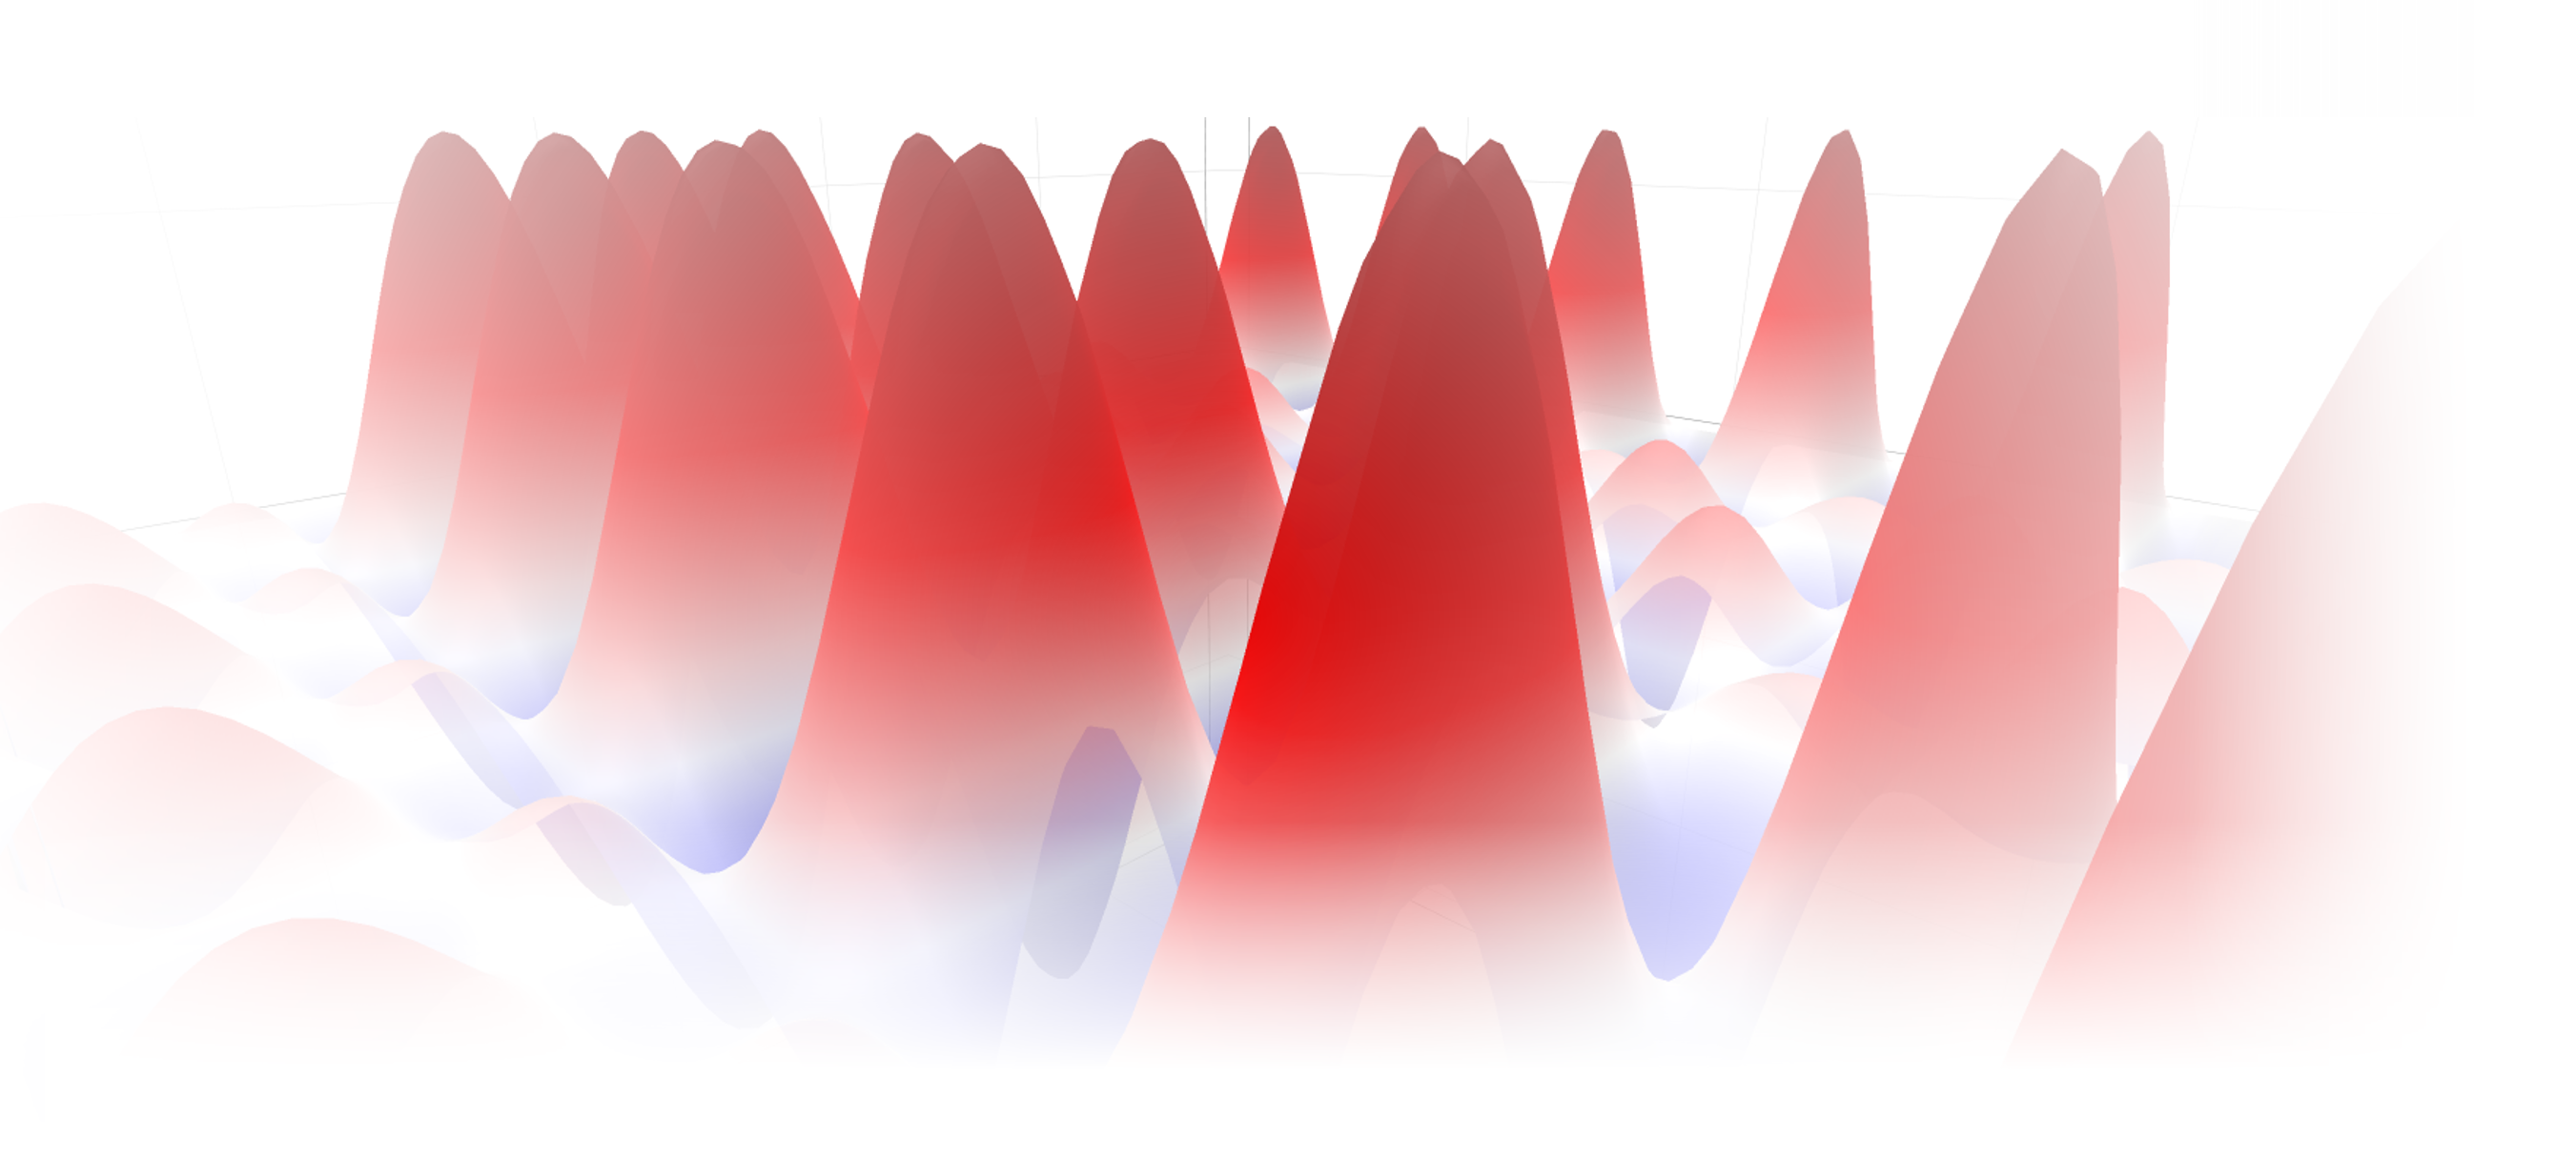
\includegraphics[width=1\textwidth, 
    trim={0cm 0 0 2.3cm}, clip]{cover_picture.png}
\end{center}

  \vfill\par
  \begin{flushright}
    \sffamily
    \@advisors\par
    \@department, ETH Z\"urich
  \end{flushright}
}

\checkandfixthelayout

\setlength{\droptitle}{-48pt}

\makeatother

% This defines how theorems should look. Best leave as is.
\theoremstyle{plain}
\setlength\theorempostskipamount{0pt}

%%% Local Variables:
%%% mode: latex
%%% TeX-master: "thesis"
%%% End:


%% Theorem environments.  You will have to adapt this for a German
%% thesis.
%% Theorem-like environments

%% This can be changed according to language. You can comment out the ones you
%% don't need.

\numberwithin{equation}{chapter}

%% German theorems
%\newtheorem{satz}{Satz}[chapter]
%\newtheorem{beispiel}[satz]{Beispiel}
%\newtheorem{bemerkung}[satz]{Bemerkung}
%\newtheorem{korrolar}[satz]{Korrolar}
%\newtheorem{definition}[satz]{Definition}
%\newtheorem{lemma}[satz]{Lemma}
%\newtheorem{proposition}[satz]{Proposition}

%% English variants
\newtheorem{theorem}{Theorem}[chapter]
\newtheorem{example}[theorem]{Example}
\newtheorem{remark}[theorem]{Remark}
\newtheorem{corollary}[theorem]{Corollary}
\newtheorem{definition}[theorem]{Definition}
\newtheorem{lemma}[theorem]{Lemma}
\newtheorem{proposition}[theorem]{Proposition}

%% Proof environment with a small square as a "qed" symbol
\theoremstyle{nonumberplain}
\theorembodyfont{\normalfont}
\theoremsymbol{\ensuremath{\square}}
\newtheorem{proof}{Proof}
%\newtheorem{beweis}{Beweis}


%% Make document internal hyperlinks wherever possible. (TOC, references)
%% This MUST be loaded after varioref, which is loaded in 'extrapackages'
%% above.  We just load it last to be safe.
% \usepackage[linkcolor=black,colorlinks=true,citecolor=black,filecolor=black, backref=page]{hyperref}
% % configure back references
% \renewcommand*{\backref}[1]{}
% \renewcommand*{\backrefalt}[4]{{%
%     \ifcase #1 Not cited.%
%           \or Cited on page~#2.%
%           \else Cited on pages #2.%
%     \fi%
%     }}

%% Helpful macros.
%% Custom commands
%% ===============

%% Special characters for number sets, e.g. real or complex numbers.
\newcommand{\C}{\mathbb{C}}
\newcommand{\K}{\mathbb{K}}
\newcommand{\N}{\mathbb{N}}
\newcommand{\Q}{\mathbb{Q}}
\newcommand{\R}{\mathbb{R}}
\newcommand{\Z}{\mathbb{Z}}
\newcommand{\X}{\mathbb{X}}

%% Fixed/scaling delimiter examples (see mathtools documentation)
\DeclarePairedDelimiter\abs{\lvert}{\rvert}
\DeclarePairedDelimiter\norm{\lVert}{\rVert}

%% Use the alternative epsilon per default and define the old one as \oldepsilon
\let\oldepsilon\epsilon
\renewcommand{\epsilon}{\ensuremath\varepsilon}

% physics stuff
% quantum states
\newcommand{\oo}{\ensuremath{\ket{11}}}
\newcommand{\zz}{\ensuremath{\ket{00}}}
\newcommand{\oz}{\ensuremath{\ket{10}}}
\newcommand{\zo}{\ensuremath{\ket{01}}}
\newcommand{\tz}{\ensuremath{\ket{20}}}
\newcommand{\zt}{\ensuremath{\ket{02}}}

\newcommand{\0}{\ensuremath{\ket{0}}}
\newcommand{\1}{\ensuremath{\ket{1}}}
\newcommand{\2}{\ensuremath{\ket{2}}}

\newcommand{\g}{\ensuremath{\ket{g}}}
\newcommand{\e}{\ensuremath{\ket{e}}}
\newcommand{\f}{\ensuremath{\ket{f}}}

% units
\newcommand{\degree}{\ensuremath{^\circ}}
% Math
% straight symbols
\renewcommand{\i}{\mathrm i}
\let\d\undefined 
\newcommand{\d}{\ensuremath{\,\mathrm d}}
\newcommand{\unit}[1]{\ensuremath{\,\mathrm{#1}}}
\newcommand{\sexp}[1]{\ensuremath{\mathrm e^{#1}}}
\newcommand{\us}{\ensuremath{\,\mu\textrm{s}}}

\newcommand{\transpose}[1]{\ensuremath{#1^\intercal}}

% quantum stuff
\newcommand{\costhamiltonian}{\ensuremath{\hat C}}
\newcommand{\ry}[1]{\ensuremath{Y(#1)}}
\newcommand{\rx}[1]{\ensuremath{X(#1)}}
\newcommand{\szsz}[2]{\ensuremath{\sigma_{#1}^z \sigma_{#2}^z}}
\renewcommand{\t}[1]{\ensuremath{T_{#1}}}

% qaoa stuff
\newcommand{\cost}{\ensuremath{C(\vec\gamma, \vec\beta)}}
\newcommand{\costh}{\ensuremath{\hat C}} % cost hamiltonian
\newcommand{\qaoa}[1]{\gls{qaoa}$_{#1}$}

\newcommand{\qaoaMeasuredState}{\ensuremath{|\vec{\gamma}, \vec{\beta}\rangle}}
\newcommand{\optimalstate}{\ensuremath{\ket{\psi_\mathrm{opt}}}}

\DeclareMathOperator*{\argmin}{arg\,min}
\DeclareMathOperator*{\argmax}{arg\,max}

% table stuff
\newcommand{\STAB}[1]{\begin{tabular}{@{}c@{}}#1\end{tabular}}
\newcommand{\HRule}{\rule{\linewidth}{0.5mm}}
\glsdisablehyper
\makeglossaries

\addbibresource{ressources/references.bib}

%% Document information
%% ====================

\title{Variational Quantum Algorithms\\ with Controlled Arbitrary Phase Gates}
\author{Nathan Lacroix}
\thesistype{Master Thesis}
\advisors{Advisors: Prof.\ Dr.\ Andreas Wallraff, Dr.\ Christian K. Andersen}
\department{Department of Solid States Physics}
\date{April 17, 2020}



\begin{document}

\frontmatter

%% Title page is autogenerated from document information above.  DO
%% NOT CHANGE.
\begin{titlingpage}
  \calccentering{\unitlength}
  \begin{adjustwidth*}{\unitlength-24pt}{-\unitlength-24pt}
    \maketitle
  \end{adjustwidth*}
\end{titlingpage}

%% The abstract of your thesis.  Edit the file as needed.
\chapter{Abstract}
Large-scale, fault-tolerant quantum computing has the potential to impact numerous fields such as medical research, material science and information security. However, near-term quantum computers will only have a limited number of quantum bits and a limited quantum circuit size that can be executed reliably.

\Glspl{vqa} mitigate the consequences of these constraints by outsourcing part of the computation to classical computers and seeking approximate -- instead of exact -- solutions.  However, the gate sequence length that can be executed still remains limited by noise, in particular decoherence. Hence, most implementations so far are restricted to problem instances that can be solved with low depth circuits. Nevertheless, real-world applications involving a higher number of qubits will most likely require deeper circuits to approximate solutions accurately. 

In this thesis, we present and implement a two-qubit gate that takes advantage of the structure in the \gls{qaoa} to reduce the sequence length of the algorithm. Namely, we extend the standard \gls{cz} to a \gls{carb} by exploiting off-resonant interaction mechanisms and careful calibration of gate length, interaction strength and dynamic phases. Our implementation of the \gls{carb} achieves an average process fidelity of 97.7\%, which we measure with process tomography.

In addition, we demonstrate the advantage of \glspl{carb} on a 3-qubit \gls{qaoa} implementation solving an exact cover problem instance. We reduce the two-qubit gate-count by 50\% and the sequence length by a factor of 3 compared to a decomposed implementation with standard CZ gates. Consequently, we achieve a higher success probability with the direct implementation (0.84 versus 0.64) and foresee an increasing advantage for larger-scale problems because  the  number  of  layers  required  for a good approximate solution typically  scales with the number of  qubits in the problem.

% TODO:
% qaoa landscape symmetries
% outlook surface 7 experiment. + check qaoa plan

\glsresetall{}

%% TOC with the proper setup, do not change.
\cleartorecto
\tableofcontents
\cleartorecto
%\listoffigures
% \cleartorecto
% \listoftables
% \cleartorecto
\newacronym{carb}{C-ARB gate}{Controlled arbitrary angle phase gate}
\newacronym{cz}{CZ gate}{Controlled phase gate}
\newacronym{vqa}{VQA}{Variational quantum algorithm}
\newacronym{qaoa}{QAOA}{Quantum approximative optimization algorithm}
\newacronym{vqe}{VQE}{Variational quantum eigensolver}
\newacronym{cqed}{cQED}{Circuit quantum electrodynamics}
\newacronym{nisq}{NISQ}{Noisy intermediate scale quantum}
\newacronym{iir}{IIR}{Infinite Impulse Response}
\newacronym{fir}{FIR}{Finite Impulse Response}
\newacronym{qpt}{QPT}{Quantum process tomography}
\newacronym{pp}{pp.}{Percentage point}
\printglossary[type=\acronymtype] 

\mainmatter

\glsresetall{}
\chapter{Introduction}
Despite the incessant progress over the last seventy years, there are still many problems today’s computers cannot solve in a realistic amount of time. While some calmly await the next generation of supercomputers, others might remain intractable for classical computers forever.

Theoretical physicist Richard Feynman popularized this observation in the early eighties. In particular, he argued that classical computers could not simulate quantum mechanics efficiently~\cite{Feynman1982SimulatingComputers}. Based on the pioneering work of Ed Fredkin and Tomasso Toffoli~\cite{Fredkin1982ConservativeLogic}, he proposed an alternative computation model exploiting fundamental properties of quantum mechanics. %Quantum computers were born --- at least, on paper.

The following decade saw a plethora of developments in quantum algorithms and quantum information 
theory~\cite{Deutsch1992RapidComputation,Shor1995Polynomial-TimeComputer,Grover1996ASearch,Simon1997OnComputation, Bernstein1997QuantumTheory,Bennett1997StrengthsComputing}. Consequently, potential applications emerged in several other fields such as information security, machine learning and optimization. In this thesis, we focus on optimization and implement an algorithm that finds an approximate solution to a combinatorial problem.

This introduction, which consists of five sections, provides the necessary material to understand the subsequent chapters. The first section introduces fundamental concepts of quantum computing and quantum information. The second provides an overview of how to realize a quantum computing experiment with superconducting circuits, the technology used in our experiments. The third section describes the constraints of near-term quantum computing resulting from imperfect implementation and suggests ways to mitigate their effect: (i) using variational quantum algorithms (VQAs) and (ii) using a more expressive gate set tailored to VQAs, thereby avoiding decomposition in their quantum circuits implementations. The fourth section further details the principles of VQAs and illustrates why the controlled arbitrary phase gate, which we implement in this thesis, is a suitable gate to avoid decomposition. Finally, the last section reports on related work and introduces the scientific contributions of this work. 

\section{Quantum computing} \label{sec:intro_quantum_computing}
Both classical and quantum computing aspire to the same goal: solving problems with algorithms. However, they differ fundamentally in the way they represent information. Classical computers encode information in binary variables, called (classical) bits. At any point in time, a bit has a state of either 0 or 1. Quantum computers rely on a generalization of this concept: the quantum bit, referred to as \textit{qubit}. A qubit has a \textit{quantum state}, $\ket{\psi}$, which, like a classical bit, is characterized by two basis states, \0 and \1\footnote{$\ket{\cdot}$ is the Dirac notation for state vectors, often used in quantum mechanics.}. However, unlike its classical counterpart, during a computation, a qubit can adopt any linear combination of these two basis states:
\begin{equation}
|\psi\rangle=\alpha|0\rangle+\beta|1\rangle, \quad \{\alpha, \beta\} \in \mathbb{C}
\end{equation}
where $\alpha, \beta$ are the (complex) amplitudes of the basis states \0 and \1, respectively. We say that the qubit can be in a \textit{superposition} of the two basis states. 

Unfortunately, quantum mechanics postulates it is impossible to examine (i.e. measure) the amplitudes of a quantum state directly. Instead, a single measurement projects the states onto only \textit{one} of the basis states with a probability equal to the squared modulus of its amplitude. In the one-qubit case, $\ket{\psi}$ yields \0 with probability $|\alpha|^2$ and \1 with probability $|\beta|^2$ and $|\alpha|^2 + |\beta|^2 = 1$. Nevertheless, it is the leveraging of interference between these amplitudes within the quantum algorithm (i.e.~\textit{before} measuring) that makes quantum computing particularly powerful.

Several qubits put together form a quantum state with even more basis states, each of which has its own amplitude. For instance, a two-qubit system encodes the quantum state $|\psi'\rangle=\alpha|00\rangle+\beta|01\rangle+\gamma|10\rangle+\delta|11\rangle$, with 4 basis states and 4 amplitudes. Generally speaking, a $N$-qubit system has $2^N$ basis states and can be in a superposition of all of them.

In close analogy to how logical gates (e.g. NOT, AND, OR) act on bits to perform classical computations, quantum algorithms consist of individual operations implemented via quantum gates, acting on single or multiple qubits. These quantum gates take a quantum state as input, shuffle the amplitudes and outputs a modified quantum state. For instance, a single-qubit gate can take $|\psi\rangle=\alpha|0\rangle+\beta|1\rangle$ and exchange the amplitudes $\alpha$ and $\beta$ such that the output is $|\phi\rangle=\beta|0\rangle+\alpha|1\rangle$. This is analogous to what a NOT gate would do to a classical bit. 

There is a convenient mathematical way to visualize how a quantum gate acts on a quantum state. Namely, using vectors and matrices. In the single qubit case, a state $|\psi\rangle=\alpha|0\rangle+\beta|1\rangle$ is encoded into the vector $\transpose{(\alpha, \beta)}$ while the gate $G$ is represented as a unitary\footnote{A complex square matrix $U$ is unitary if its conjugate transpose $U^\dagger$ is also its inverse, i.e.\ if $U^\dagger U=U U^\dagger=I$.} $2\times2$ matrix, 
\begin{equation}
G = 
\begin{pmatrix}
a_0 & a_1 \\
b_0 & b_1
\end{pmatrix}
\end{equation}
in which the coefficients in the first and second column indicate how the gate affects the basis states \0 and \1 respectively. In particular, if the input state is \0, which can be written as $ \transpose{(1,0)}$, then the output state is $a_0\ket0 + b_0\ket1$ and if the input state is \1 then the output state is $a_1\ket0 + b_1\ket1$. In the more general case, if the input state is $\ket\psi = \transpose{(\alpha, \beta)}$, then the output state $\ket\phi$ is given by the product
\begin{equation}
    \ket\phi = G \ket \psi = 
    \begin{pmatrix}
a_0 & a_1 \\
b_0 & b_1
\end{pmatrix} \cdot 
\begin{pmatrix}
\alpha \\
\beta 
\end{pmatrix}
\end{equation}
For the single-qubit gate exchanging $\alpha$ and $\beta$, $G = \left(\transpose{(0,1)}, \transpose{(1,0)}\right)$ such that
\begin{equation}
\ket\phi = G \ket \psi = 
\begin{pmatrix}
0 & 1 \\
1 & 0
\end{pmatrix} \cdot 
\begin{pmatrix}
\alpha \\
\beta 
\end{pmatrix} =  
\begin{pmatrix}
\beta \\
\alpha 
\end{pmatrix}
\end{equation}
A similar technique is used for two-qubit gates. They are described by $4\times4$ matrices multiplying vectors with 4 entries (one for each basis state).

Remarkably, a very small set of single- and two-qubit gates, called \textit{universal gate set}, is sufficient to implement any quantum computation with arbitrarily many qubits because any high level instruction can be decomposed to a list of gates belonging to that universal gate set~\cite{Nielsen2000QuantumInformation}\footnote{A similar concept also exists in classical computing, stating that NAND gates alone form a universal set.}.

The existence of universal gate sets is very valuable for building a quantum computer because it implies we can perform quantum computation with few distinct gates implemented in hardware. Nevertheless, building a quantum computer remains an immense challenge. Indeed, it requires to create and manipulate objects displaying quantum mechanical properties, which typically do not materialize at the scale we live in. One option, as we shall see in the next section, consists in mimicking atoms and their quantum mechanical properties with superconducting circuits.

\section{Quantum computers with superconducting circuits} \label{sec:intro_building_qc}
Since the advent of quantum information theory, many technologies have been explored to build quantum computers: ions trapped in an electromagnetic trap~\cite{Monroe1995DemonstrationGate}, semiconductor quantum dots~\cite{Loss1998QuantumDots}, photons and linear optics~\cite{Knill2001AOptics}, superconducting circuits~\cite{Blais2004CavityComputation}, and many more. While each technology has its pros and cons, in this thesis we focus on superconducting circuits, one of the leading technology platform ~\cite{Kjaergaard2019SuperconductingPlay} which we use in our experiments.

In superconducting circuits, qubits are represented by artificial atoms, realized as superconducting electrical circuits with discrete energy levels. Typically, the first two levels are chosen to represent the basis states \0 and \1  while the remaining ones are ignored. The core idea is to create a quantum harmonic oscillator using an $LC$-circuit ($L$ is an inductor and $C$ is a capacitor). This circuit has a resonance frequency $\omega = 1/\sqrt{LC}$ which corresponds to the frequency of the transition between the energy levels in the system. In a quantum mechanical picture, the resulting harmonic potential has quantized energy levels spaced by the energy quantum $\hbar\omega$~\cite{Kjaergaard2019SuperconductingPlay}, where $\hbar$ is the reduced Planck constant. 

Provided the temperature is sufficiently low and there is little dissipation, the energy levels of the oscillator are distinguishable and addressable. However, the equidistant spacing between energy levels prevents from using directly the quantum harmonic oscillator as a qubit. Indeed, while trying to induce a transition from \0 to \1 by injecting an energy quantum, we might induce a transition from \1 to \2 if there is already an excitation in the system. Hence, we cannot restrict the computational space to the first two levels as desired for binary quantum computing. 

To circumvent this problem, we create an anharmonic energy potential by using a non-linear inductor called a Josephson tunnel junction~\cite{Vion2003QuantumProcessing}. The junction's inductance depends non-linearly on the magnetic flux flowing through it. The introduced anharmonicity enables the separate addressing of each transition with the  matching transition frequency. 

There are several ways to obtain a Hamiltonian with discretized, anharmonic energy levels using a Josephson junction. One of them consist in creating a superconducting island with one side connected to ground via a Josephson junction, and the other coupled via a capacitor to a voltage source~\cite{Bouchiat1998QuantumPair, Nakamura1999CoherentBox}. 

When the voltage source is unbiased, the system lies in the ground state, \0, also referred to as \g. By increasing the voltage of the source, we polarize the island with the capacitor until a charge quantum\footnote{These charge quanta are called Cooper-pairs and form at very low temperature when two electrons of opposite spin in the metal pair up to form a bosonic state. At sufficiently low temperatures, all valence electrons in the metal form Cooper-pairs and they can all occupy the same ground state.} tunnels (without loss) through the Josephson junction onto the island to restore charge balance. The energy stored in the capacitor after the tunneling is called the charging energy, $E_C$, and the energy stored in the junction is called the Josephson energy, $E_J$. 
If the gate voltage is subsequently removed, there is \textit{charge offset} on the island and the system is out of equilibrium, i.e., there is one excitation in the system (\1 or \e). Because the state of the system depends on the amount of charge on the island, this implementation is called the \textit{charge qubit}.

In our experiments, we use the \textit{transmon}~\cite{KochCharge-insensitiveBox} -- a special case of the charge qubit -- that operates in the regime $E_J/E_C \approx 50$ to mitigate environmental charge noise~\cite{KochCharge-insensitiveBox, Oliver2013MaterialsBits}. In addition, we use a SQUID to control the Josephson energy with an external magnetic flux, $\Phi$.
The total energy required to introduce excitations in the system depends on the energies $E_J(\Phi)$ and $E_C$. For the first transition energy~\cite{KochCharge-insensitiveBox},
\begin{equation} \label{eq:qubit_frequency}
    E_{\ket{1}}/\hbar \approx \omega_{\ket{1}} \approx \sqrt{8E_J(\Phi) E_C} - E_C
\end{equation}

Transition frequencies for frequency tunable transmons are typically located in the micro-wave part of the electromagnetic spectrum (4-8 GHz). Therefore, we use microwave pulses tuned to the appropriate transition frequency to perform the single-qubit gates between the state \0 and \1.

Due to the inherent environmental noise, implementing perfect quantum gates represents an immense challenge in practice. Other experimental considerations further complicate the implementation of quantum computing: for instance, \textit{decoherence}, the process of loosing quantum information encoded in a system over time due to undesirable interactions with the environment\footnote{We typically distinguish between \textit{relaxation}, characterized by the time constant \t{1}, which relates to the spontaneous decay of excitation captured in the system after some time, and \textit{dephasing}, characterized by the time constant \t{2}$^{*}$ , which relates to the loss of information about the phase of the system.}, puts a hard bound how many quantum operations can be executed reliably. 
In addition, information stored in qubits cannot be copied~\cite{Wootters1982ACloned} which prevents the use of cloning and majority voting as error correcting scheme. Instead, quantum error correction codes employing many physical qubits to encode the state of few logical qubits~\cite{Gottesman2010AnComputation, DiVincenzo1996Fault-TolerantCodes, Fowler2012SurfaceComputation} are required to achieve fault-tolerant quantum computing. 

These experimental complications will impose limitations on what (noisy) quantum computers achieve in the near future. Nevertheless, the steady improvement of coherence times and multi-qubit chip control over the last two decades now enable quantum computations which challenge the most powerful classical supercomputers~\cite{Arute2019QuantumProcessor}.  We are thus at the dawn of a new and exciting quantum computing stage that physicists have named the \textit{noisy intermediate-scale quantum} era.

\section{The noisy intermediate-scale quantum era}
While Google recently claimed having performed a task on a 53-qubit quantum computer that would take extremely long time on a supercomputer~\cite{Arute2019QuantumProcessor}, full-scale fault-tolerant quantum computing is still a distant dream. The pivotal period we just entered, called the \gls{nisq} era~\cite{Preskill2018QuantumBeyond}, entails two major limitations on near-term quantum computers:
\begin{enumerate}
    \item The performance of quantum devices is severely limited by noise. There are many possible sources of noise. However, a dominant one is decoherence. For fixed coherence times, quantum computers can only execute a limited number of operations (quantum gates) before quantum information is lost. We say that decoherence limits the \textit{depth} of the quantum circuit.
    \item The number of qubits available for computation is limited. Fabricating high quality and multi-qubit quantum processors is a laborious task. Therefore, we expect near-term quantum computers to have fewer than 1000 physical qubits.
\end{enumerate} 

Bearing in mind those limitations, how can we make best use of current quantum computers? 

Firstly, we shall implement quantum algorithms, such as \textit{\glspl{vqa}}~\cite{Moll2017QuantumDevices}, which are believed to cope better with \gls{nisq} limitations. \Glspl{vqa} are suited for the \gls{nisq} era because they outsource part of the algorithm which does not require quantum properties to classical computers. Therefore, available qubits are used more efficiently and part of the computation is carried out by classical computers which do not suffer from decoherence. In addition, \glspl{vqa} are intrinsically less sensitive to noise because they seek approximate solutions (instead of exact solutions). Hence, coherent errors may be partially compensated for by the classical optimizer such that they lead to worse approximate solutions but typically do not ruin the whole computation. Nonetheless, errors accumulating over time (such as decoherence) will severely limit the performance of \glspl{vqa}.

Secondly, we  can significantly reduce the time required to execute \glspl{vqa} on quantum computers by tailoring the available gate set on the quantum computer to match typical operations performed by \glspl{vqa}. The conceptual underlying principle is presented in Fig.~\ref{fig:intro_quantum_circuits}. When generating a quantum circuit to solve a mathematical problem, the first step consists of formulating the problem we want to solve in a way which the \gls{vqa} can take it as input. Next, we receive a list of instructions from the algorithm to follow in order to solve the problem. These instructions are passed on to the quantum computer. However, the quantum computer can only perform a restricted set of operations based on the available gates implemented in hardware. Therefore, it might be necessary to decompose some operations into a longer sequence of available gates.

In particular, decomposition occurs when a \gls{vqa} is implemented on a quantum computer with a so-called standard gate set. This set comprises of the most commonly implemented two-qubit gates such as the CNOT-, CZ- and SWAP-gate. They receive most attention because a small subset of them, such as the CNOT-gate (or SWAP-gate) combined with arbitrary single-qubit gates, forms a universal gate set which allows to implement any instruction, as discussed in Section~\ref{sec:intro_quantum_computing}. However, the decomposition of these instructions can be arbitrarily long, which is a major drawback, especially during the \gls{nisq} era.

\begin{figure}[ht]
    \centering
    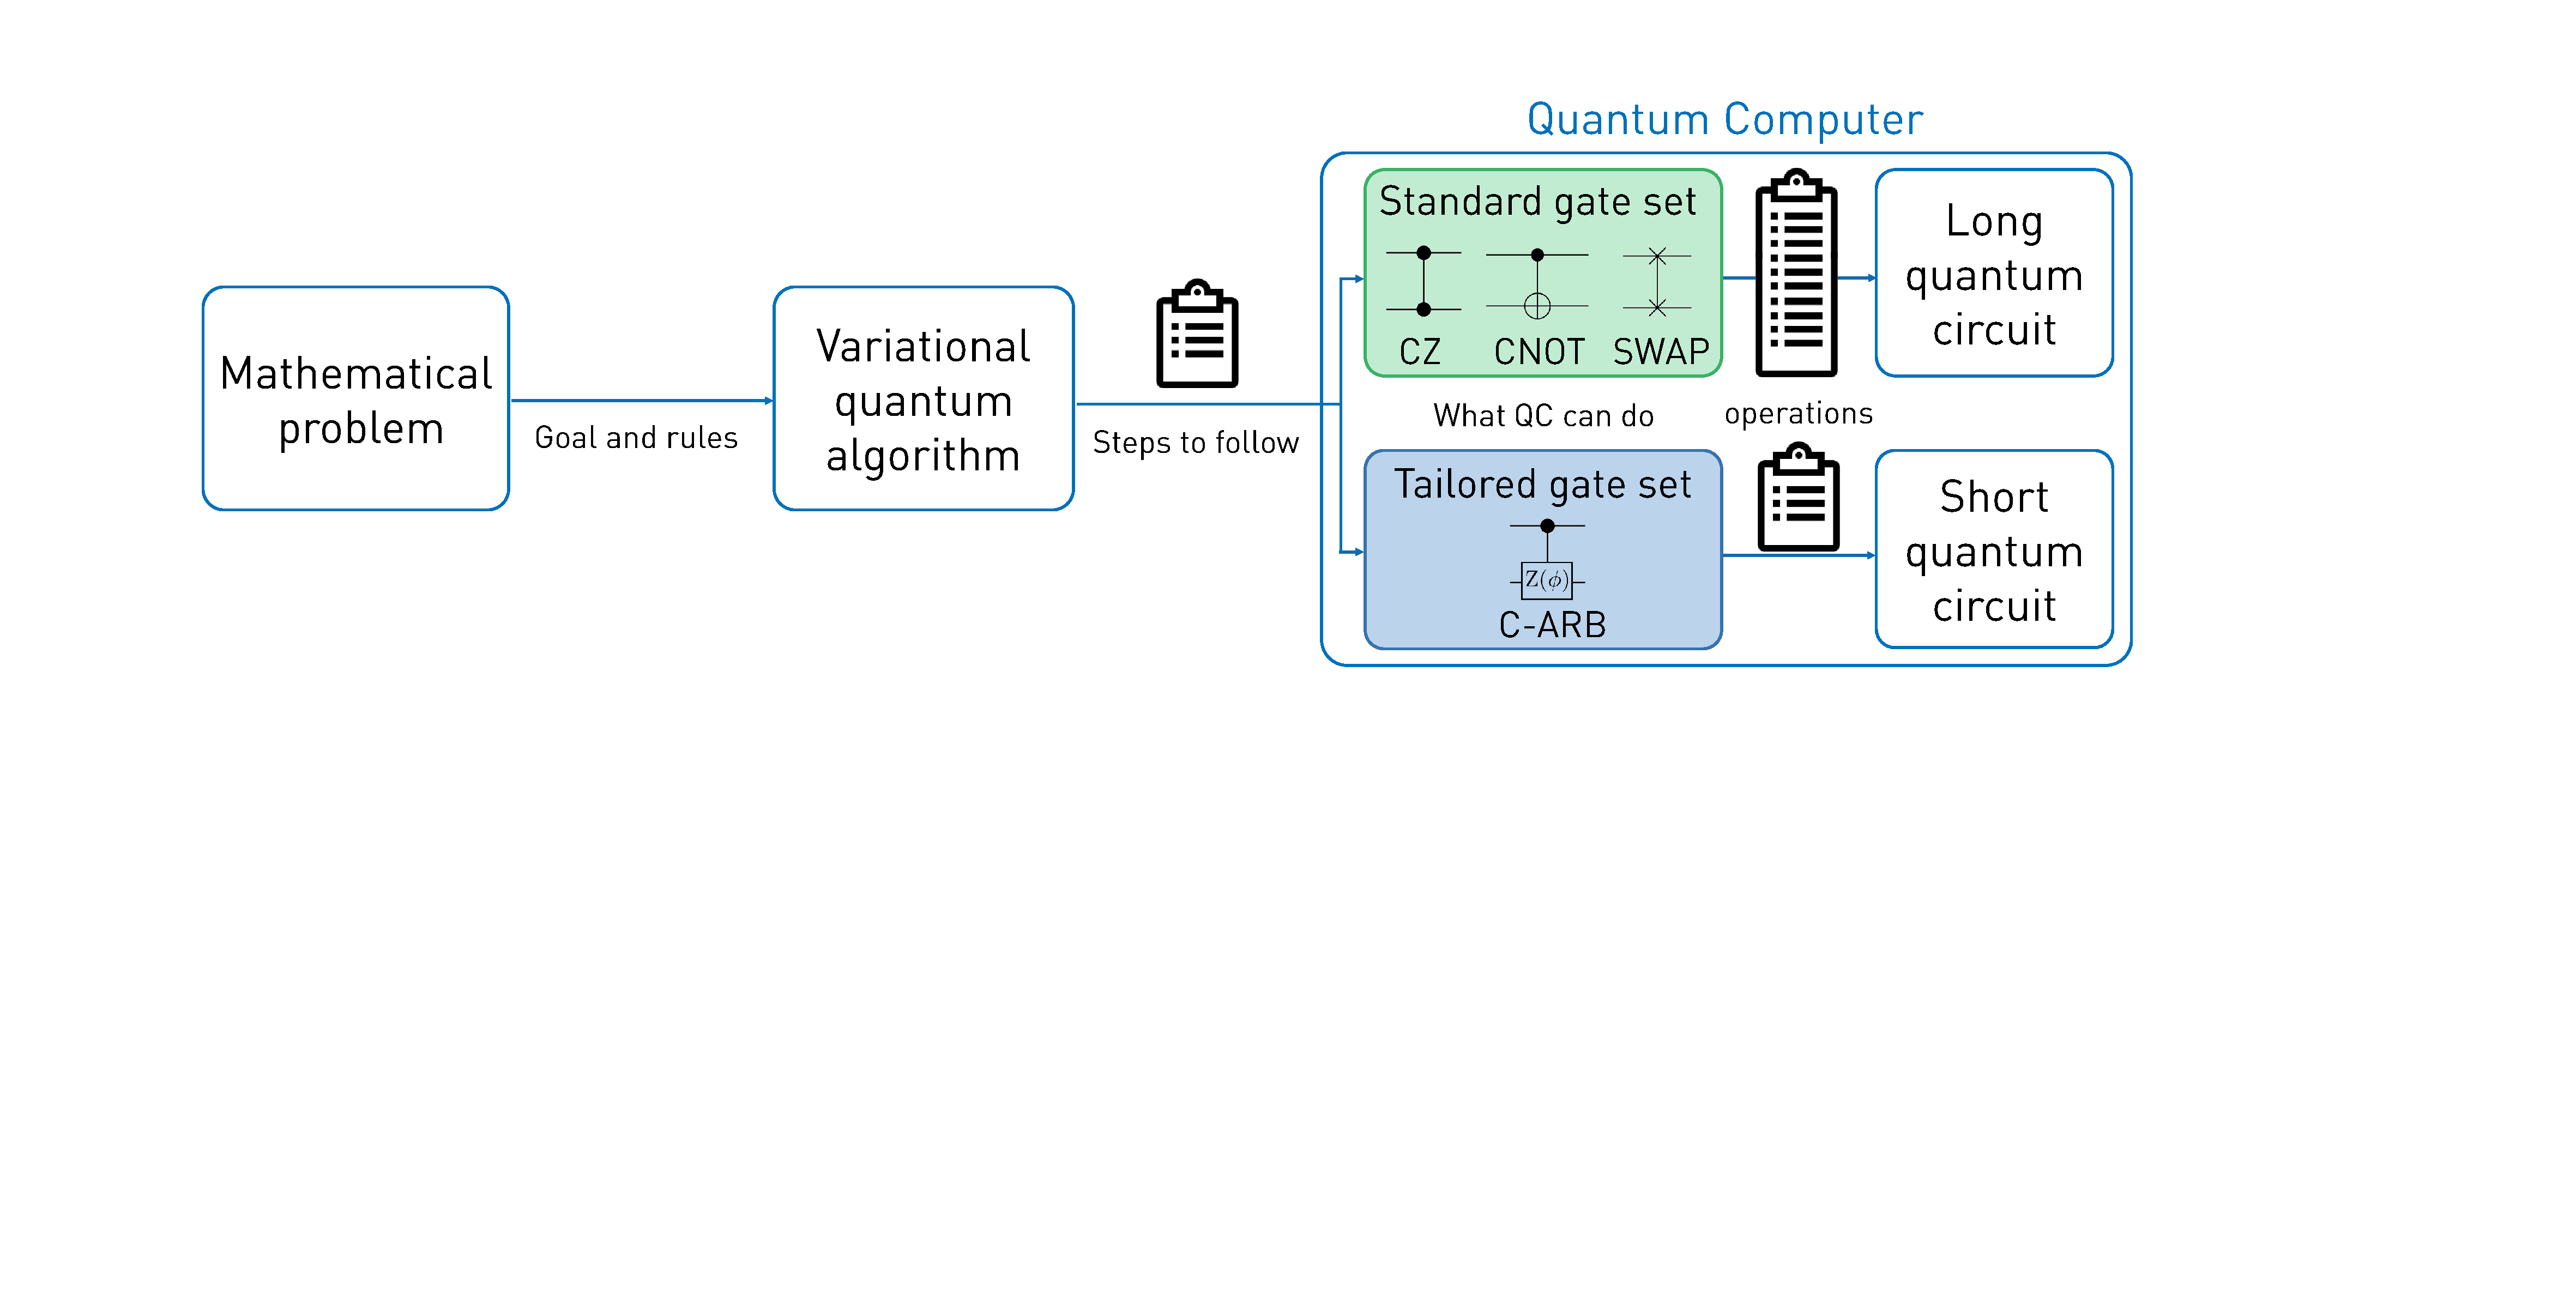
\includegraphics[width=\textwidth, trim={5cm 18cm 10cm 2cm},clip]{quantum_circuits_v3.pdf}
    \caption{Conceptual process flow to generate quantum circuits.}
    \label{fig:intro_quantum_circuits}
\end{figure}%\todo{harmonize color with vqa figure}

In this thesis, we present and characterize the \gls{carb}, an expressive two-qubit gate which avoids decomposition of instructions for various \glspl{vqa}. In the next section, we detail the basic working principle of \glspl{vqa} and explain why \glspl{carb} reduces the depth of their quantum circuits implementations.

\section{Variational quantum algorithms}
\glsreset{vqa}
\Glspl{vqa} encompass hybrid quantum-classical algorithms which leverage a quantum computer prepare a state in a large state space that would be exponentially hard to prepare classically, while the rest of the computation is executed by a classical computer~\cite{Moll2017QuantumDevices}. The two most prominent \glspl{vqa} are the \gls{vqe}~\cite{Peruzzo2014AProcessor}, which finds approximate solutions to quantum chemistry problems and the \gls{qaoa}~\cite{Farhi2014AAlgorithm}, which applies to generic combinatorial optimization problems. Their basic working principle is illustrated in Fig.~\ref{fig:intro_vqa}.

\begin{figure}[b]
    \centering
    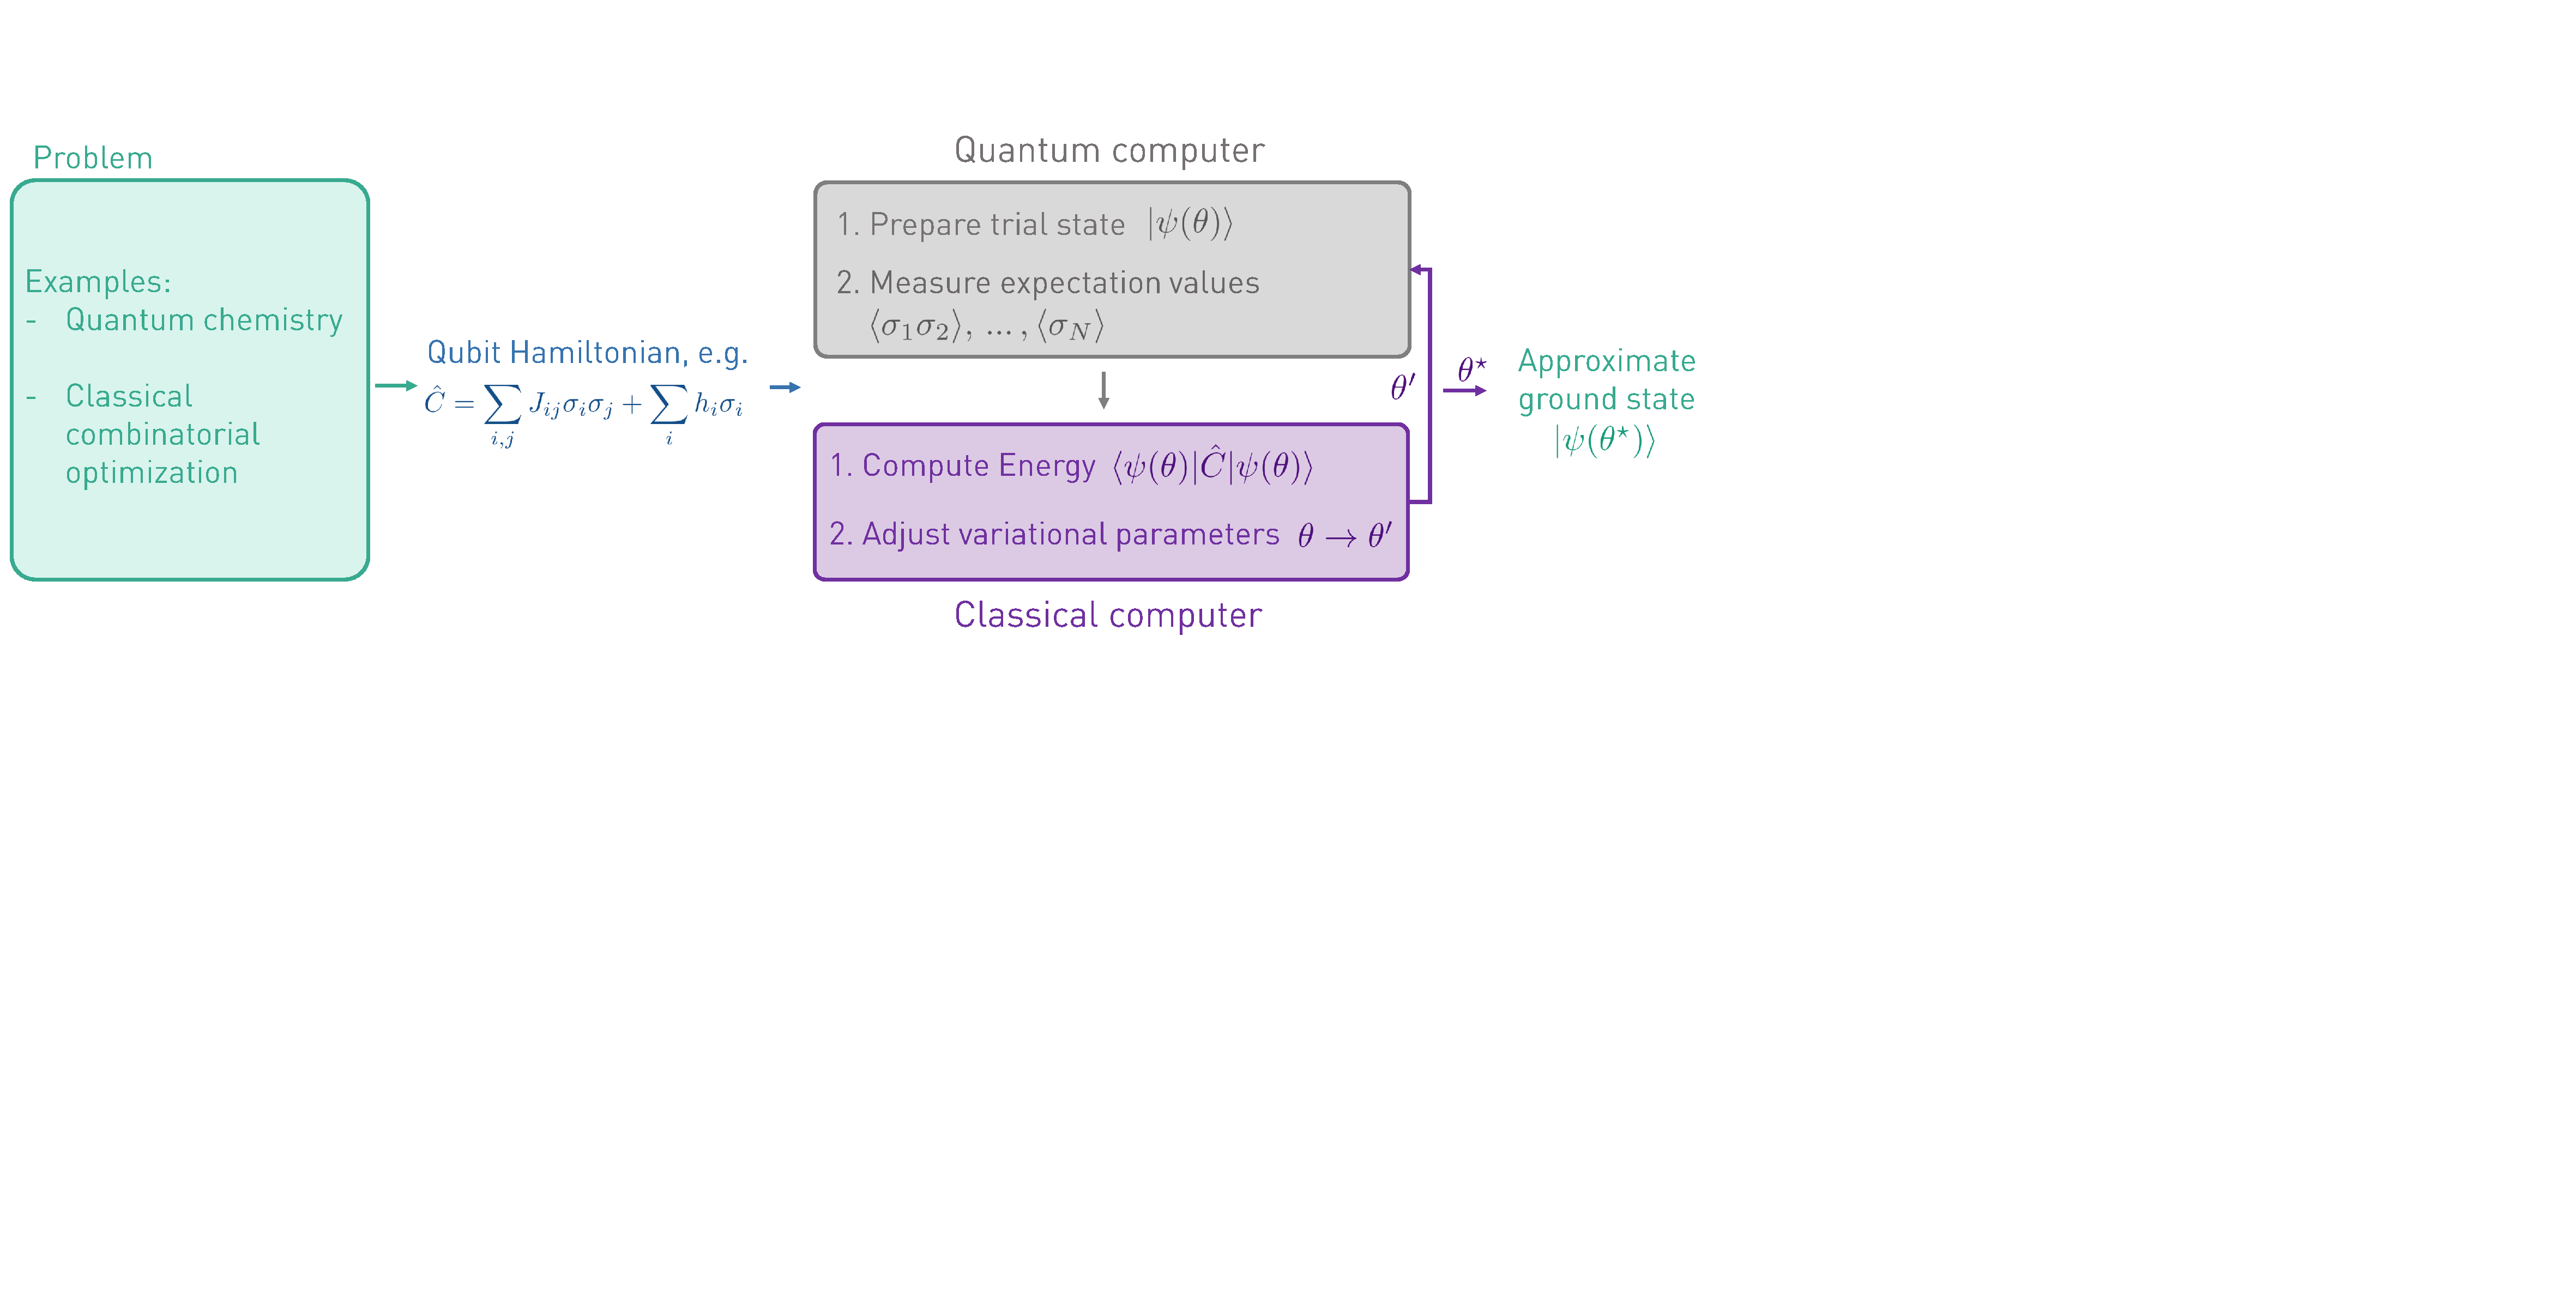
\includegraphics[width=\textwidth, trim={0cm 18cm 26cm 2cm},clip]{variational_quantum_algorithms_v2.pdf}
    \caption{Basic principle of a \gls{vqa}. A problem is mapped onto a qubit (cost) Hamiltonian $\hat C$,  where each term consists of tensor-products of individual Pauli operators~\cite[p.~65]{Nielsen2000QuantumInformation}. In this case, we picture an Ising-like Hamiltonian. The quantum computer prepares a parametrized trial state, $\ket{\psi(\theta)}$ and measures the expectation values of each term in $\hat C$. Based on the expectation value of the cost Hamiltonian, $\langle \psi(\theta) | \hat C |  \psi(\theta) \rangle$ a classical computer adjusts the circuit parameters, $\theta$, to minimize $\langle \hat C \rangle$.}
    \label{fig:intro_vqa}
\end{figure}

For both algorithms, the original problem is mapped in polynomial time to a (qubit) cost Hamiltonian, $\hat C$, such that its solution coincides with finding the ground-state energy of that Hamiltonian. Thereafter, the search for the ground-state is performed using both a quantum and a classical computer. 

The quantum computer generates a trial state $|\psi(\theta)\rangle$ based on variational parameters $\theta$ and the cost Hamiltonian. Repeated single shot measurements allow to estimate the expectation values for each term of the cost Hamiltonian. Based on the expectation value of the total energy, $\langle \psi(\theta) | \hat C |  \psi(\theta) \rangle$,  a classical optimizer suggests new variational parameters $\theta'$ to minimize the smooth function of the expectation value of the energy. At convergence, the final state $\ket{\psi(\theta^\star)}$ with corresponding final variational parameters $\theta^\star$ constitutes an approximate solution for the ground-state, from which an approximate solution to the original problem is deduced. 

The quality of the approximation strongly depends on the depth of the  quantum circuits. Indeed, \glspl{vqe} and \gls{qaoa} mimic a \textit{continuous} time evolution of the system with \textit{discrete} steps to find its ground-state~\cite{Lloyd1996UniversalSimulators} (see Section~\ref{sec:qaoa_relation_to_adiabiatic_computing} for a detailed discussion about \gls{qaoa}'s relationship to the time evolution of a quantum system). Each additional layer -- or step -- in the quantum circuit improves the quality of the approximation but also increases the number of operations and hence the depth of the circuit. 

In \gls{qaoa}, each layer $l$ directly includes the unitary evolution due to the cost Hamiltonian for a time defined by the variational parameter $\theta_l$: $U_{C_l}(\theta_l) = \sexp{-\i\hat C \theta_l}$. When $\hat C$ is an Ising-like Hamiltonian in the $z$-basis~\cite{Lucas2014IsingProblems},  two-qubit terms in $\hat C$ result in unitaries of the form $\sexp{-\i\,\phi}$ where $\phi = \theta_l\sigma_i^z\sigma_j^z$. Since the parameter $\theta_l$ can adopt continuous real values, the operation includes the addition of an (arbitrary) phase $\phi$ on the two-qubit state $\ket{11}_{ij}$, which cannot be implemented with a standard \gls{cz} which adds a $\pi$ conditional phase. Therefore, early implementations of \gls{qaoa} decomposed two-qubit terms into two two-qubit gates and additional single qubit gates (see Section~\ref{sec:qaoa} for more details). 

\section{Related work}
The idea of using expressive gate sets for \glspl{vqa} recently inspired research groups at IBM, Rigetti Computing and Google, see Table \ref{tab:qaoa_experiments}, entries 1-3. In 2019, Ganzhorn et al.\ implemented exchange-type gates tailored for quantum chemistry simulation~\cite{Ganzhorn2019Gate-EfficientComputer} with a fidelity of $\sim95\%$. In the same year, Abrams et al.\ implemented a more general XY-entangling gate~\cite{Abrams2019ImplementationPulse} with median fidelity of 97.4\%. This gate family directly applies to quantum chemistry simulations, and a combination of two gates of this family also reduces decomposition in quantum circuits for combinatorial optimization. Finally, Foxen et al.\ ~\cite{Foxen2020DemonstratingAlgorithms} implemented both an arbitrary iSWAP-type gate and an arbitrary conditional phase gate which they concatenate to achieve similarly general interactions as with the XY-entangling gate. They report a two-qubit Pauli error of $3.8\times 10^{-3}$.

All three research groups implemented gates for superconducting qubits. Ganzhorn et al.\ and Foxen et al.\ implemented tunable couplers-based gates~\cite{McKay2016UniversalBus, Chen2014QubitCoupling} while Abrams et al.\ realized parametric entangling gates~\cite{Reagor2018DemonstrationLattice} with one fixed and one tunable transmon.

At the time of writing, Abrams et al.\ is the only group that implemented the \gls{qaoa} using expressive gates~\cite{Abrams2019ImplementationPulse}. In combination with standard CZ-gates, their parametrized XY-gates enable an impressive two-qubit gate count reduction of $\sim$30\%, which they briefly illustrate for a one-layer \gls{qaoa} implementation of a four-qubit, all-to-all connected MaxCut problem graph.

However, several groups implemented the \gls{qaoa} with standard gates prior to Abrams et al.'s work, see Table \ref{tab:qaoa_experiments}, entries 4-6. In 2017, Otterbach et al.\ solved a clustering problem on 19 superconducting qubits~\cite{Otterbach2017UnsupervisedComputer}. The problem could be solved using a single layer of the \gls{qaoa} such that the decomposition -- which occurs in each layer -- did not strongly affect the performance of the algorithm. In 2019, Pagano et al.\ estimated the ground state energy of a transverse field Ising model with tunable long-range interactions with 20 trapped ions and a two-layer \gls{qaoa}~\cite{Pagano2019QuantumSimulator}. Similarly, the best theoretical approximate solution with two layers is only $\sim1.5\%$ away from the ground state with respect to the full energy scale. Bengtsson et al.\ were the first to implement a problem requiring a two-layer \gls{qaoa} on (two) superconducting qubits~\cite{Bengtsson2019QuantumProcessor}. 

\begin{table}
\small
\centering
\caption{Summary and comparison of publications on expressive gate sets (top three entries), \gls{qaoa} experiments (entries 4 to 6) and this work. Entries are ordered chronologically based on their publication date.}
\label{tab:qaoa_experiments}
\resizebox{\textwidth}{!}{%
\begin{threeparttable}
\begin{tabular}{ p{3.5cm} p{4cm} p{1.cm} p{2cm} p{1cm} p{4cm}}
\toprule
Authors & Main message & qubits & Problem  & layers\tnote{*}  & gate implementation \\ 
\midrule
Ganzhorn et al.~\cite{Ganzhorn2019Gate-EfficientComputer} & Exchange-type gates + VQE demo & 2 & H$_2$-molecular energy & - & parametric, tunable coupler based \\
Abrams et al.~\cite{Abrams2019ImplementationPulse} & XY-interaction gate family + QAOA demo & 4 & MaxCut & 1 (?) & parametric \\
Foxen et al.~\cite{Foxen2020DemonstratingAlgorithms} & Continuous SWAP and phase gates & 2 & - & - & tunable coupler based (gmon device) \\
\midrule
Otterbach et al.~\cite{Otterbach2017UnsupervisedComputer} & First QAOA implementation & 19 & MaxCut & 1 (1) & parametric CZ gates  \\
Pagano et al.~\cite{Pagano2019QuantumSimulator} & Analog implementation of Ising model with ions & up to 40 & Generic Ising & 2 (1) &  Analog long-range Ising \\ 
Bengtsson et al.~\cite{Bengtsson2019QuantumProcessor} & Solve a simple problem instance with high success probability using QAOA & 2 & Exact cover & 2 (2) &  parametric CZ gates with tunable coupler\\
\midrule
This work & Demonstrate the advantage of using \glspl{carb} for \gls{qaoa} & 3 & Exact cover & 9 (3) &  fixed coupling \glspl{cz} and \glspl{carb}\\
\bottomrule
\end{tabular}
\begin{tablenotes}
\item[*]Implemented layers and between brackets the number of layers required to solve the problem with a success probability larger than 95\%.
\end{tablenotes}
\end{threeparttable}}

\end{table}

In this thesis, we present the first in-depth experimental analysis of the advantage of expressive gates, i.e.\  \glspl{carb}, for the implementation of \glspl{vqa}. In Chapter \ref{ch:carb}, we describe the calibration and characterization procedure of a \gls{carb} for fixed-coupling, frequency-tunable transmons~\cite{DiCarlo2009DemonstrationProcessor} with an average process fidelity of $\sim 97.7\%$. In Chapter \ref{ch:qaoa}, we use \glspl{carb} to obtain a 50\% two-qubit gate count reduction on  a combinatorial problem exploiting the connectivity of our three-qubit device. We also implement for the first time a problem requiring three \gls{qaoa} layers to be solved with high success probability. In addition, we compare quantitatively on this problem the performance obtained with the direct implementation of the \gls{carb}, and its decomposed alternative. We show that, the \gls{qaoa} utilizing the direct implementation solves the problem with greater success probability. 
 
\chapter{Calibrating and Characterizing Controlled Arbitrary Phase Gates} \label{ch:carb}
\glsreset{carb}
This chapter details the concepts, calibration and characterization of \glspl{carb}. We start by explaining how this gate family can be seen as an extension of standard conditional phase gate (\glspl{cz}). Next, we demonstrate the implementation of a \gls{carb}, allowing us to reach continuous conditional phase in the range $[0, 2\pi[$. We describe the calibration procedure of the gate on qubit 2 and 3 of our quantum processor presented in Appendix~\ref{app:setup}. Next, perform quantum process tomography and evaluate the process fidelity as a function of conditional phase. By exploiting the 3-level readout discussed in Appendix~\ref{ch:qutrit_readout}, we then characterize conditional- and dynamic phase errors and leakage. We compare these phase errors and leakage values to the ones obtained with a \gls{cz} implemented on the same qubits.

\section{Theoretical description} \label{sec:c_arb_theory}
In this section, we derive the unitary evolution of the \gls{carb} and explain the physical mechanisms behind its implementation. The goal is to obtain a unitary operator $U_{\textrm{C-ARB}}$ in a two-qubit subspace which adds a controllable phase $\phi$ to the \oo{} state, 
\begin{equation} \label{eq:carb_unitary}
    U_{\textrm{C-ARB}}=
    \begin{pmatrix}
{1} & {0} & {0} & {0} \\
{0} & {1} & {0} & {0} \\
{0} & {0} & {1} & {0} \\
{0} & {0} & {0} & {e^{-\i \phi}}
\end{pmatrix}
\end{equation}

We obtain such unitary by exploiting the same effect as for the \gls{cz}, namely the collection of geometric phase on the \oo{} state due to the interaction of the \oo{} level and the non-computational \tz{} level~\cite{Strauch2003QuantumQubits, DiCarlo2009DemonstrationProcessor}. As pictured in Fig.~\ref{fig:carb_theory}(a),  the \oo{} and \tz{} levels hybridize strongly when they are brought close to resonance. In this regime, we can approximate their interaction as a two-level system where the ground (excited) state is the \oo{} (\tz{}) state. The system is characterized by the Hamiltonian
\begin{equation}
    \hat H/\hbar= \omega_{\ket{11}} \oo{} \bra{11} + \omega_{\ket{20}} \tz{} \bra{20} + J( \oo{}\bra{20}+ \tz{}\bra{11})
\end{equation}
where  $\omega_{\ket{11}}$ ($\omega_{\ket{20}}$) is the frequency of the energy level \oo{} (\tz{}), and $J$ is the fixed coupling strength between the two levels which is a chip design parameter fixed during fabrication. The first and second term in the Hamiltonian correspond to the energy in the \oo{} and \tz{} level respectively. The third term represents the coupling energy between the two levels in which the excitation is transferred from one level to the other and vice-versa. 

The same Hamiltonian can conveniently be written in matrix form with basis vectors \oo{} and \tz{},
\begin{equation}
\hat{H}/\hbar=
\begin{pmatrix}
\omega_{\oo} & J \\
J & \omega_{\tz}
\end{pmatrix}
\end{equation}
We shift the zero energy to $\omega_{\oo}$  and define the frequency detuning between the two levels $\Delta = \omega_{\tz}- \omega_{\oo}$ such that $\hat H$ becomes
\begin{equation}
\hat{H}/\hbar=
\begin{pmatrix}
0 & J \\
J & \Delta
\end{pmatrix}
\end{equation}

From Schr\"odinger's equation, it follows that the time evolution of an arbitrary state $\ket{\psi}$ in the \oo-\tz{} subspace is given by $|\psi(t)\rangle = U(t)\ket{\psi}$ where $U(t) = \sexp{-\i \hat H/\hbar t}$ is the unitary evolution of the Hamiltonian. Specifically, the unitary $U(t)$ is defined as,
\begin{equation}
\begin{split}
    &U(t) = \\
& \begin{pmatrix}
 \sexp{-\frac{1}{2} \i t \Delta } \left(\cos \left(\frac{1}{2} t \Tilde{J} \right)+\frac{\i \Delta  \sin \left(\frac{1}{2} t \Tilde{J}\right)}{\Tilde{J}}\right) & -\frac{2 \i e^{-\frac{1}{2} \i t
   \Delta } J \sin \left(\frac{1}{2} t \Tilde{J}\right)}{\Tilde{J}} \\
 -\frac{2 \i e^{-\frac{1}{2} \i t \Delta } J \sin \left(\frac{1}{2} t \Tilde{J}\right)}{\Tilde{J}} & \sexp{-\frac{1}{2} \i t \Delta }
   \left(\cos \left(\frac{1}{2} t \Tilde{J}\right)-\frac{\i \Delta 
   \sin \left(\frac{1}{2} t \Tilde{J}\right)}{\Tilde{J}}\right) \\
\end{pmatrix}
\end{split}
\end{equation}
where we have defined for clarity $\Tilde{J} := \sqrt{4J^2+\Delta^2}$ which we call the \textit{effective exchange coupling}.

When starting with an excitation in the \oo{} state (the ground-state of this two-level subsystem), the \oo{} population oscillates coherently as the excitation is swapped back and forth between the \oo{} and the \tz{} state,
\begin{equation}
P_{\oo{}}(t) = \mathrm{Tr}\left(U(t)\ket{11}\bra{11}U^\dag(t)\right) = \frac{\Delta ^2+2 J^2 (\cos \left(t \sqrt{4J^2+\Delta^2}\right)+1)}{4J^2+\Delta^2}
\end{equation}
with an oscillation period of $2\pi/\Tilde{J}$. 

The population as function of frequency detuning $\Delta$ and interaction time $t$ results in a Chevron pattern shown in Fig.~\ref{fig:carb_theory}(b). For the operating point of the \gls{cz}, $\Delta = 0$, the population is given by $P_{\oo{}} = \frac{1}{2} + \frac{1}{2}\cos{2Jt}$. This corresponds to a complete population exchange between the \oo{} and the \tz{} state and with an oscillation period of $\pi/J$. By contrast, $\Delta \neq 0$ results in a partial population exchange between the \oo{} and the \tz{} state. The oscillation period is also reduced due to the detuning $\Delta$ in the denominator. 

\begin{figure}
    \centering
    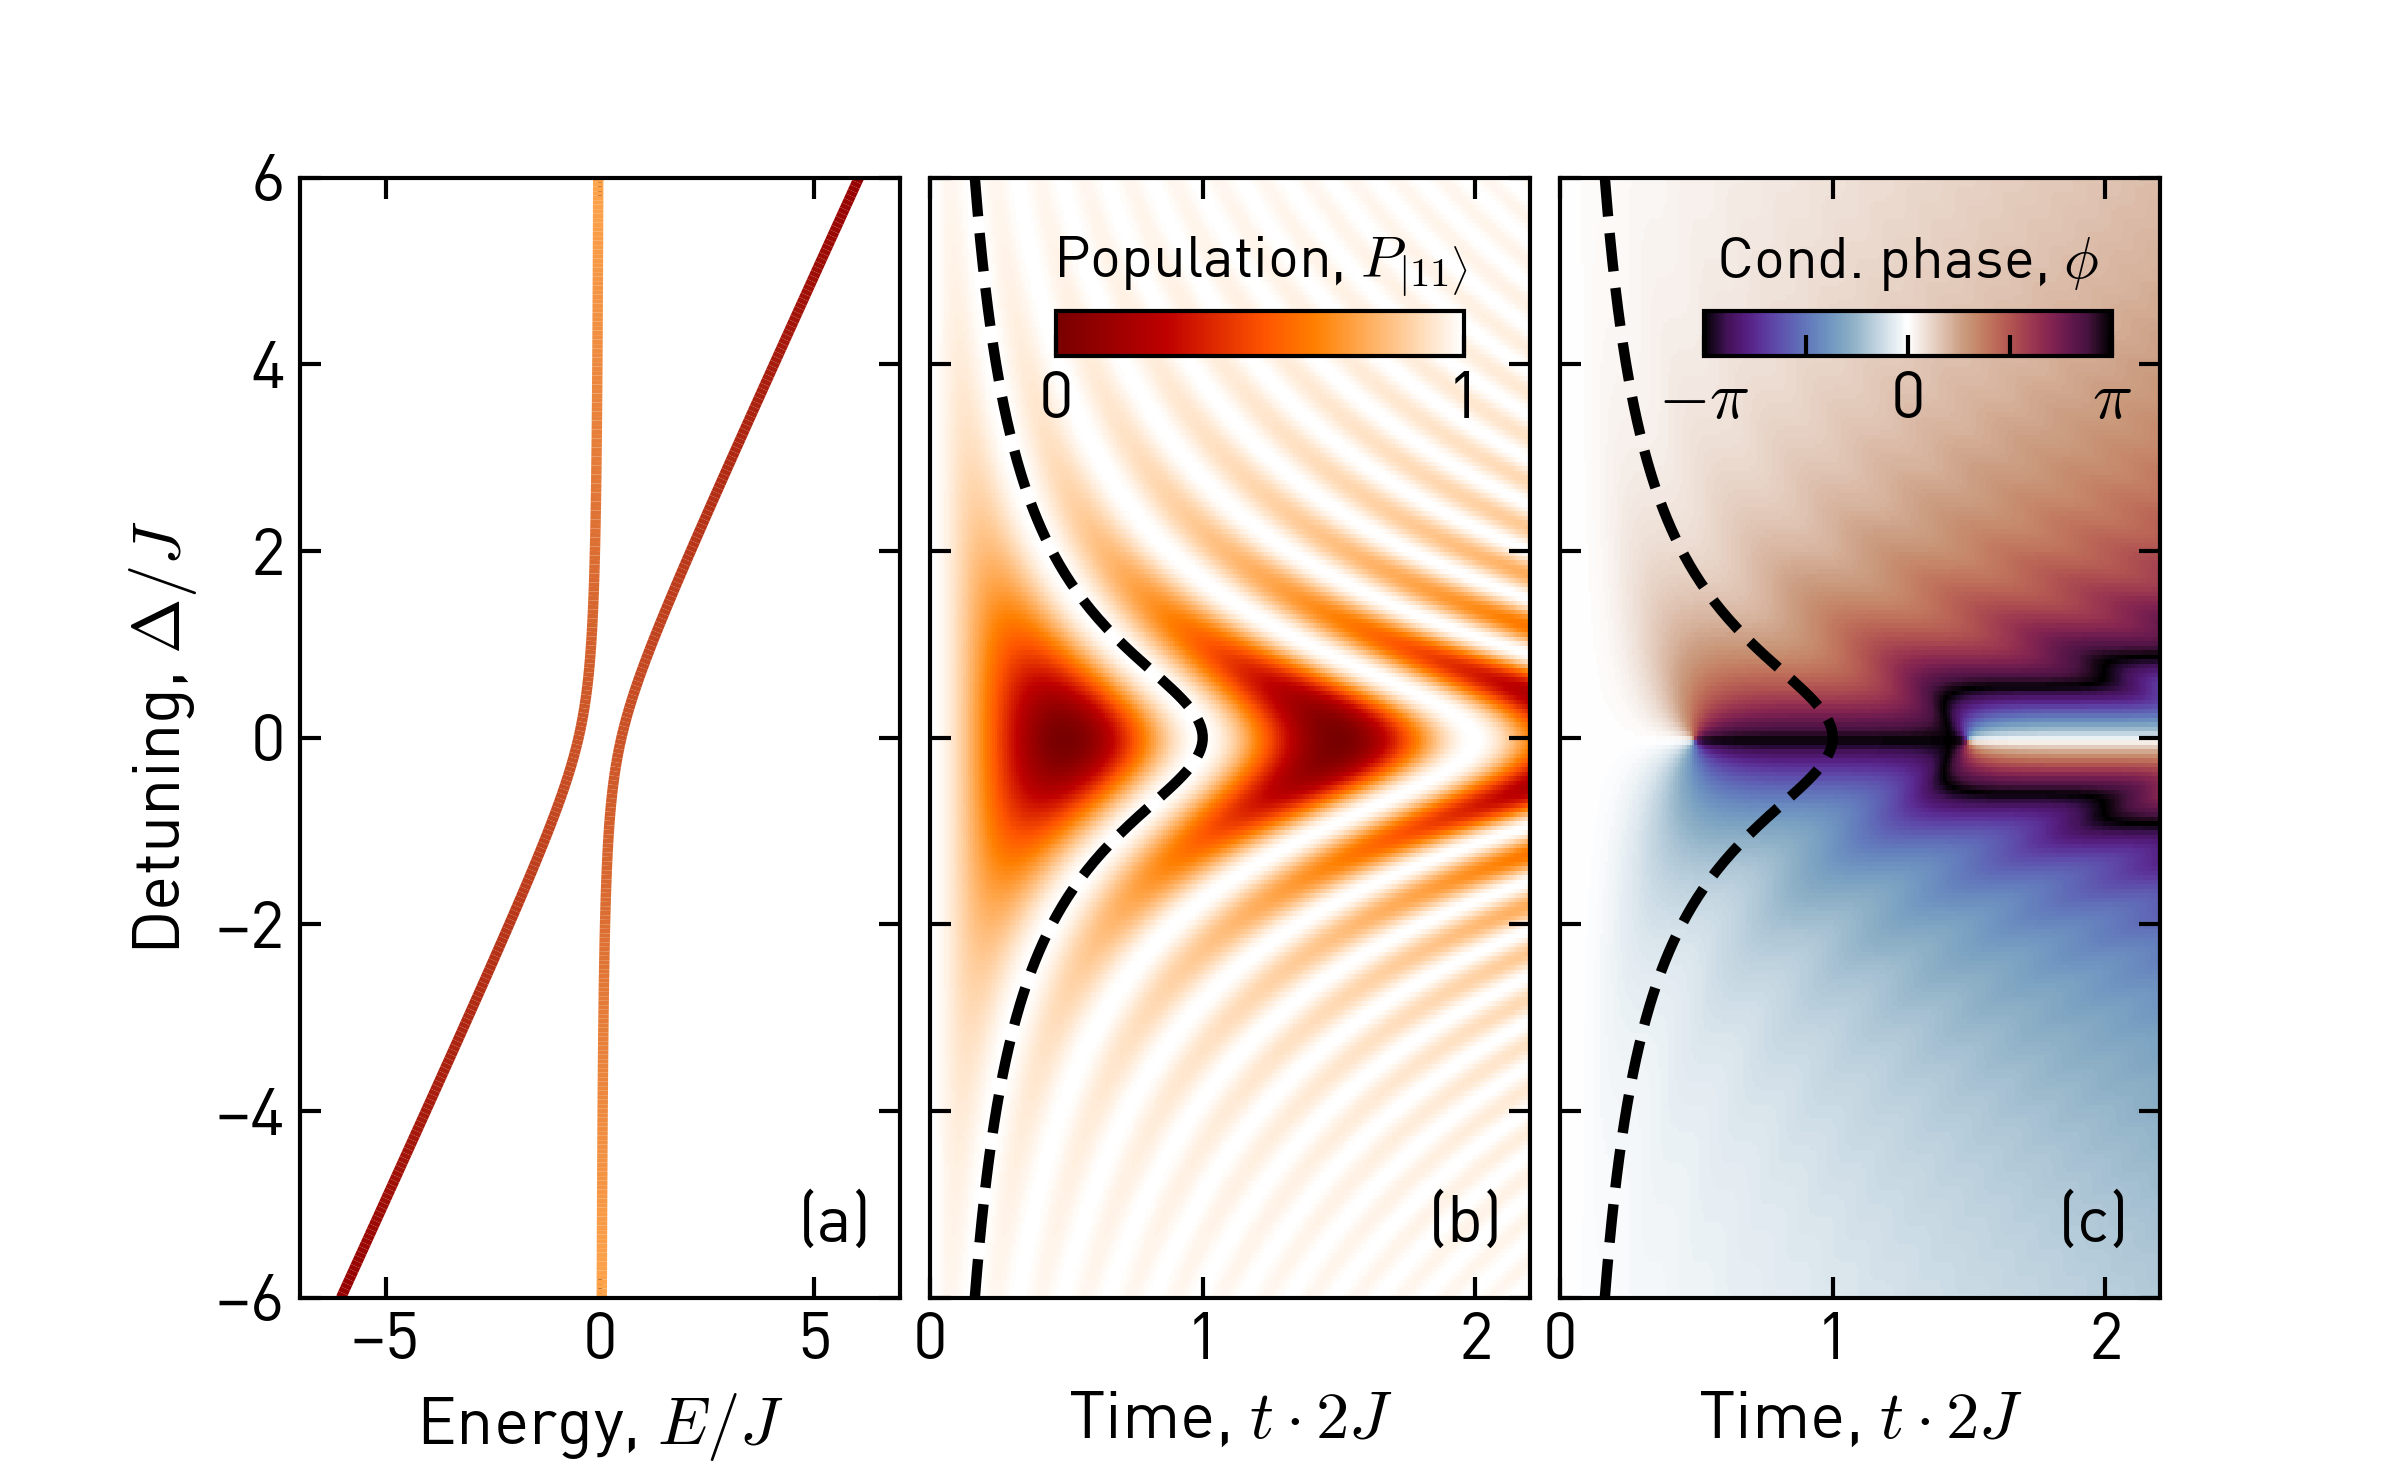
\includegraphics[width=1\textwidth]{chapters/carb_gate/figs/ch4_carb_theory_c3_20200312_095516.png}
    \caption{Simulation of the \gls{carb} as a generalization of the \gls{cz}. (a) Avoided crossing between the \oo{} (brown) and the \tz{} (orange) energy levels as function of detuning. (b) Population of the \oo{} state as function of frequency detuning $\Delta$ and interaction time $t$ (in units of $J$) visualizing the coherent population exchange due to hybridization. The dashed line corresponds to the frequency detunings and gate lengths resulting in the first maximum in population recovery in the computational subspace. (c) Conditional phase acquired on the \oo{} state resulting from the interaction of the two levels. We reach all conditional phases between 0 and $2\pi$ by sweeping the detuning and adapting the time accordingly to ensure population recovery (dashed line). }
    \label{fig:carb_theory}
\end{figure}

The gate length must be an integer multiple of the oscillation period to ensure a unitary operation within the computational subspace (i.e.\ full population recovery). In Fig.~\ref{fig:carb_theory}(b), we highlight (dashed line) the first oscillation period which corresponds to the shortest possible gate length as a function of the frequency detuning,
\begin{equation} \label{eq:carb_t_gate}
    t_{\textrm{C-ARB}} = \frac{2\pi}{\sqrt{4J^2+\Delta^2}}
\end{equation}

In  Fig.~\ref{fig:carb_theory}(c),  we illustrate the acquired conditional phase, $\phi$, as a function of detuning and gate length. For the gate lengths $t_{\textrm{C-ARB}}$, the corresponding phase on the \oo{} state acquired by the closed loop state evolution is
 \begin{equation} \label{eq:ch4_acquired_cond_phase}
     \phi = \mathrm{Arg}\Big(\bra{11}U(t_{\textrm{C-ARB}})\oo\Big) =  \pi \cdot \left( 1 + \frac { \Delta } { \sqrt { \Delta ^ { 2 } + 4 J ^ { 2 } } } \right)
 \end{equation}
which spans the interval $[0, 2\pi[$ for a sufficiently large detuning sweep, see dashed line in Fig.~\ref{fig:carb_theory}(c). As expected, a zero detuning yields a conditional phase of $\pi$ and therefore corresponds to the standard \gls{cz}.

In practice, we achieve these timed interactions with flux pulses\footnote{In fact, we apply a \textit{voltage} pulse at the output of the \gls{awg} and the latter creates a current in the flux line which results in magnetic flux through the SQUID loop} which shift the transition frequency of the individual qubits. For a gate in the off-state, we ensure $|\Delta|\gg J$ such that the acquired conditional phase is small. Ideally, the acquired phase should be zero but in practice it is not due to the residual $ZZ$-coupling between the \oo{} and the \tz{} state. To turn on the gate, we apply a square flux pulse with amplitude $a$ and length $l$ to one of the qubits via its flux line. The pulse shifts the \oo{} state non-adiabatically close to the \tz{} state. 

As mentioned in Section~\ref{sec:intro_building_qc}, the flux affects the Josephson energy~\cite[Eq.~2.18]{KochCharge-insensitiveBox}, 
\begin{equation}\
    E_J(a) = E _ { J , \max } \sqrt { \cos ^ { 2 } \left( \frac{\pi}{\Phi_0} \frac { \partial \Phi } { \partial V } a \right) + d ^ { 2 } \sin ^ { 2 } \left( \frac{\pi}{\Phi_0}\frac { \partial \Phi} { \partial V } a \right) }
\end{equation}
where $d$ is the asymmetry between the junctions in the SQUID loop of the transmon, $ \partial \Phi /\partial V $ is the flux sensitivity (voltage to flux conversion parameter), $\Phi_0 = h/2e$ is the superconducting flux quantum and $E _ { J , \max }$ is the maximal junction energy. 

In turn, the Josephson energy shifts the qubit transition frequency as defined by Eq.~\eqref{eq:qubit_frequency} such that
\begin{equation} \label{eq:carb_theory_freq01}
    \omega_{|01\rangle}(a) \simeq \sqrt{8  E _ { J , \max } \sqrt { \cos ^ { 2 } \left( \frac{\pi}{\Phi_0}\frac { \partial \Phi } {  \partial V } a \right) + d ^ { 2 } \sin ^ { 2 } \left( \frac{\pi}{\Phi_0}\frac { \partial \Phi} { \partial V } a \right)} E_{C}}-E_{C} 
\end{equation}
where we approximate $|E_c|$ to be equal to the anharmonicity $|\alpha_2|$ of the fluxed transmon~\cite[Eq. 2.12]{KochCharge-insensitiveBox}. 
The frequency detuning, $\Delta$, as function of the flux pulse amplitude is then simply
 \begin{equation}\label{eq:carb_detuning}
\begin{aligned} 
\Delta(a) & = \omega _ { | 20 \rangle } - \omega _ { | 11 \rangle } \\ 
& = 2 \omega _ { | 10 \rangle } - \alpha _ { 1 } - \left( \omega _ { | 10 \rangle } + \omega _ { | 01 \rangle }(a) \right) \\ 
& = \omega _ { | 10 \rangle } - \alpha _ { 1 } - \omega _ { | 01 \rangle }(a) 
\end{aligned}
\end{equation}
where $\alpha_1$ is the anharmonicity of the  transmon which is not fluxed.

It follows that varying the amplitude of the flux pulse indeed controls the frequency detuning between the \oo{} and the \tz{} state, which in turn controls the collected phase on the \oo{} state. To ensure full population recovery in the computational subspace, the length of the flux pulse must be $t_{\textrm{C-ARB}}$ which can be related back to the amplitude of the flux pulse by combining Eq.~\eqref{eq:carb_t_gate}, \eqref{eq:carb_theory_freq01} and \eqref{eq:carb_detuning},
\begin{equation} \label{eq:carb_t_gate_from_ampl}
\begin{split}
    &t_{\textrm{C-ARB}}(a)\simeq\\
    &   \frac{2\pi}{\sqrt{4J^2+\left(\omega _ { | 10 \rangle } - \alpha _ { 1 } - \sqrt{8  E _ { J , \max } \sqrt { \cos ^ { 2 } \left( \frac{\pi}{\Phi_0}\frac { \partial \Phi } {  \partial V } a \right) + d ^ { 2 } \sin ^ { 2 } \left( \frac{\pi}{\Phi_0}\frac { \partial \Phi} { \partial V } a \right)} \alpha_2} - \alpha_2 \right)^2}}
\end{split}
\end{equation}
In Section~\ref{sec:carb_calibration}, we fit Eq.~\eqref{eq:carb_t_gate_from_ampl} to experimental data to estimate $J$, $ \partial \Phi/ \partial V $ and $d$ and thereby also the expected conditional phase using Eq.~\eqref{eq:ch4_acquired_cond_phase}.

In addition to the conditional phase, the flux pulse also results in a dynamic phase $\phi_D$ on the fluxed qubit,  because it takes the qubit out of its rotating frame~\cite{DiCarlo2009DemonstrationProcessor},
\begin{equation} \label{eq:carb_dyn_phase}
    \phi_D = \int_0^l{(\omega(t)-\omega_{\textrm{park}})\d t}
\end{equation}
where $\omega(t)$ and $\omega_{\textrm{park}}$ denote the instantaneous qubit frequency during the pulse and the frequency at parking position\footnote{The parking position refers to the frequency of the qubit when the gate is off. We typically choose it to be where the derivative of the frequency with respect to flux is 0 to minimize the charge noise, a point we call the "sweet spot"~\cite{Vion2003QuantumProcessing}}, respectively. We compensate for this single-qubit phase shift with a virtual $Z$ gate after the \gls{carb}.

While the \gls{cz} is composed of from a single detuning and gate length, the \gls{carb} requires a careful interpolation of distinct detunings and corresponding gate lengths to span all possible conditional phases with high \oo{} population recovery. In addition, since the qubit frequency excursion depends on $\Delta$, dynamic phases have to be calibrated for all possible detuning/gate-length pairs. We detail the calibration procedure of these three continuous parameters in the next section.

\section{Calibration} \label{sec:carb_calibration}
This section describes the calibration procedure of a \gls{carb} using a square flux pulse on qubit 2 and 3 of the device presented in Appendix~\ref{app:setup}. To account for the finite rise-time and ensure a stable voltage at the output of the \gls{awg}, we filter the square pulse with a 1\unit{ns} Gaussian kernel. The calibration of the \gls{carb} consists of three measurements, illustrated in Fig.~\ref{fig:ch4_calibration_carb}.

First, we calibrate the pulse lengths to ensure maximum population recovery. We prepare the \oo{} state and perform a two-dimensional sweep of the flux pulse amplitude and length. For each amplitude and length, we measure the \1{} population of qubit 2 after the flux pulse using 3-level readout, yielding the Chevron pattern shown in Fig.~\ref{fig:ch4_calibration_carb}(a). Brighter areas correspond to high
level population of qubit 2, indicating the population is fully swapped back from the \2{} level into the computational subspace. To find the pulse lengths corresponding to the first period of the population exchange, we fit the \1{} population oscillation to a cosine for each pulse amplitude of the two-dimensional sweep. We then retrieve the pulse length corresponding to the first maximum of the population recovery.

We fit the pulse lengths corresponding the maximum population recovery to Eq.~\eqref{eq:carb_t_gate_from_ampl} to extract the flux sensitivity $\frac { \partial \Phi} { \partial V }$, the asymmetry between the junctions in the SQUID loop $d$  and the coupling strength $J$ between the \oo{} and \tz{} states. The fit is shown as a dashed line in Fig.~\ref{fig:ch4_calibration_carb}(a). We obtain a flux sensitivity of $\frac { \partial \Phi} { \partial V } / \Phi_0 = 0.34 \pm 0.01 \unit{\frac{1}{V}}$, an asymmetry of $0.7884 \pm 0.0003$ and a coupling of $J/2\pi =  4.72 \pm 0.05 \unit{MHz}$, all of which are consistent with previous characterization of this device~\cite{Andersen2019, Andersen2019a}.

Next, we measure the conditional phase as function of flux pulse amplitudes (see Fig.~\ref{fig:ch4_calibration_carb}(b)) while adapting the pulse length to maximize population recovery (see Fig.~\ref{fig:ch4_calibration_carb}(a), black circles). If necessary, pulse length is interpolated linearly between the calibration points of the pulse length calibration. The colored flux pulses shown in the pulse scheme in Fig.~\ref{fig:ch4_calibration_carb}(e) correspond to the diamond-shaped data points of respective color in ~\ref{fig:ch4_calibration_carb}(b). Using the parameter values obtained from the fit in Fig.~\ref{fig:ch4_calibration_carb}(a), we compute the expected conditional phase from  Eq.~\eqref{eq:ch4_acquired_cond_phase} and plot it in dashed line in Fig.~\ref{fig:ch4_calibration_carb}(b). The measured conditional phase saturates at a value of different than 0 due the phase acquired via the a residual $ZZ$-coupling of $\alpha_{ZZ} = 400\unit{kHz}$ over the period the pulse length and buffers (25ns) that separates the two $R_x^{\pi/2}$-pulses. 

Finally, we measure the dynamic phase the fluxed qubit acquires during its frequency excursion (see Fig.~\ref{fig:ch4_calibration_carb}(c)) with the pulse scheme presented in Fig.~\ref{fig:ch4_calibration_carb}(f)). With the approximation that its frequency is constant over the entire pulse at the value given by Eq.~\eqref{eq:carb_theory_freq01}, we compute the expected dynamic phase from Eq.~\eqref{eq:carb_dyn_phase} and show it with a dashed line. This measurement requires a high number of calibration points, as the dynamic phase grows rapidly as a function of detuning yet can only be measured in the $[0, 2\pi[$ interval (a minimum of 3 points per $[0, 2\pi[$ interval are required to ensure correct unwrapping). In Fig.~\ref{fig:ch4_calibration_carb}(c), only one out of three points is shown for clarity. 
\begin{figure}[H]
    \centering
    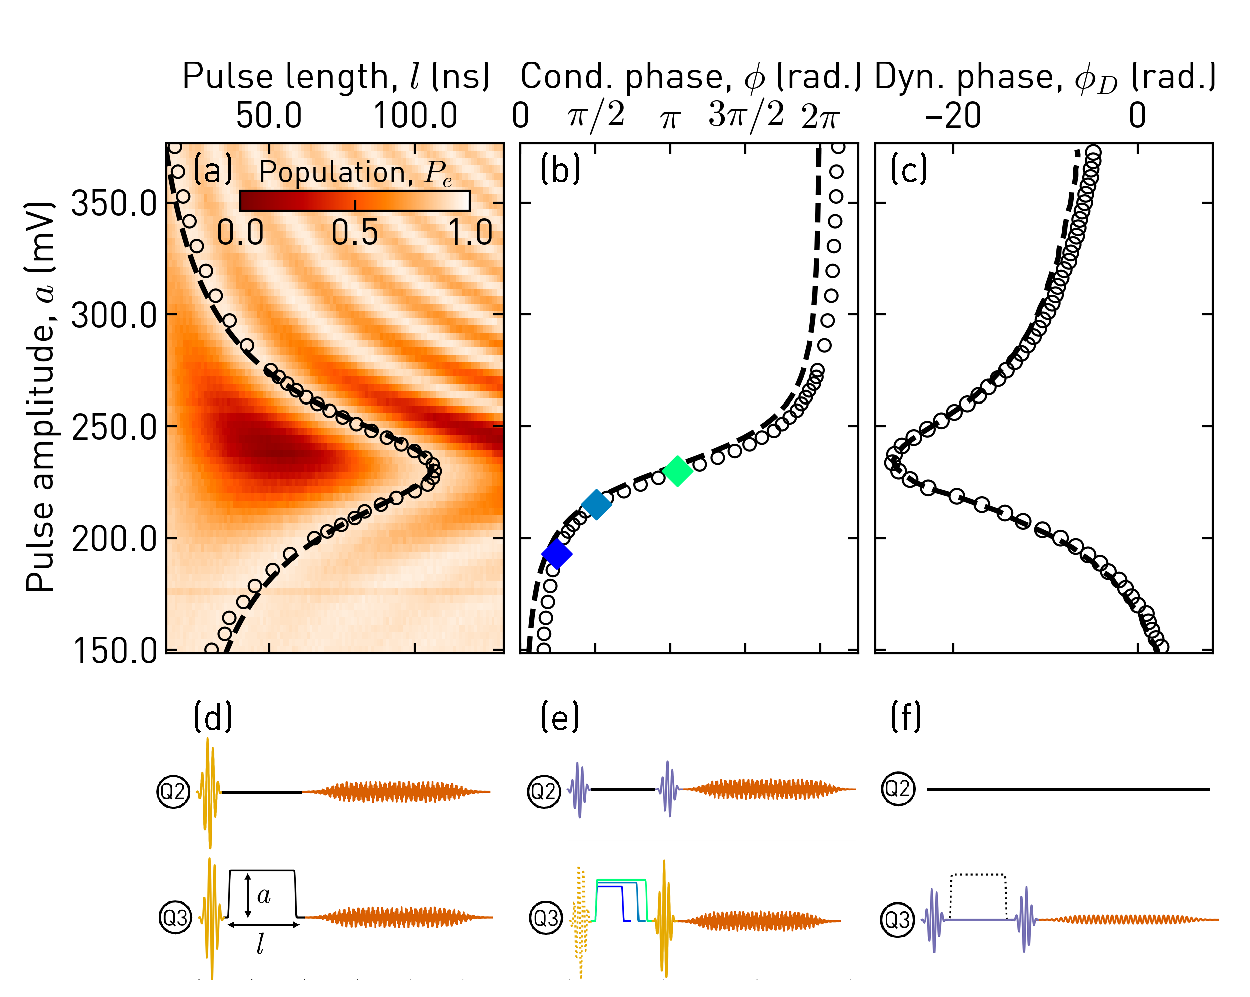
\includegraphics[width=\textwidth]{chapters/carb_gate/figs/ch4_carb_calibration_20200406_215519.pdf}
    \caption{Three calibration measurements (a, b, c) of a \gls{carb} and their corresponding pulse schemes (d, e, f).  (a) Qubit 2 \e{} level population as function of the flux pulse amplitude and length. The inset details the pulse scheme: the \oo{} state is prepared, the flux pluse (black) is  applied to qubit 3, the two qubits are read out with a multiplexed readout pulse. The scattered points correspond to the amplitudes and lengths used to calibrate the conditional phase (see b). The dashed line corresponds to the fit to the theoretical model. (b) Conditional phase as function of flux pulse amplitude. The amplitude sampling is not uniform to account for the non-linearity of the conditional phase. The dashed line indicates the phase predicted of the model (see main text for details).  (c) Unwrapped dynamic phase of qubit 3 as function of pulse amplitude. Only one out of three data point is shown for clarity.  The dashed line corresponds to the dynamic phase predicted by theory (see main text for details). (d) Pulse scheme corresponding to the two-dimensional parameter sweep shown in (a). The \oo{} state is prepared with two single-qubit $R_x^\pi$ (yellow), followed by the flux pulse (black) of amplitude $a$ and length $l$, and finally a readout pulse (orange). (e) Pulse scheme to measure conditional phase (see b). The phase is measured on qubit 2 with a Ramsey experiment (two $R_x^{\pi/2}$ pulses (purple)), while qubit 3 is fluxed once with and once without preceding single-qubit $R_x^{\pi}$ (dashed yellow). The difference between the two measurements yields the conditional phase. The different flux pulse colors result in the conditional phases indicated with diamonds of corresponding color in (b). (f) The dynamic phase is measured by comparing the phase of the qubit via a Ramsey experiment with and without flux pulse (dashed black).}
    \label{fig:ch4_calibration_carb}
\end{figure}

Due to flux cross-talk between the flux lines, the qubit staying at its parking position also acquires a non-zero dynamic phase. However, the latter is not calibrated, as flux cross-talk between the flux line of qubit 1 (3) and qubit 2 is smaller than 2\% (3\%) for the two two-qubit gates considered in this report~\cite{Andersen2018SampleB4QP3}.

The calibration time of the \gls{carb} on qubits 2 and 3 amounts to approximately 2 hours and 45 minutes i.e.\ about 5 to 8 times slower than a full calibration of a \gls{cz}. The high-resolution, two-dimensional amplitude/gate length sweep last for 1 hour, whilst for the conditional phase measurement (45 calibration points) requires 15 minutes, and the dynamic phase, 1 hour and 30 minutes. The following actions would reduce the calibration time:
\begin{itemize}
    \item[--] Use the active reset scheme discussed in Section~\ref{sec:active_reset}. This scheme allows an increase of the repetition rate by a factor of 5-10 leading to a total measurement time of 20-40 minutes.
    \item[--] Use a non-linear amplitude sampling for the dynamic phase based on the theoretical model. Namely, have an adaptable spacing between amplitudes at which the dynamic phase is calibrated based on whether the model predicts a large or small increase in dynamic phase. This would reduce the number of measurement point for the dynamic phase calibration by a factor of $\sim2$, compared to a dense linear pulse amplitude spacing.
    \item[--] Rewrite the dynamic phase measurement such that all waveforms are uploaded on the AWGs at once, instead of one at the time. This would reduce communication overhead.
\end{itemize}
Implementing these changes could in principle reduce the calibration time to under 20min per gate. Parallel tune up of two-qubit gates has the potential to decrease the calibration time of the device even further. 

In this section, we demonstrated the ability to calibrate a \gls{carb}. The next section details the characterization of the gate.

\begin{comment}
In addition to the pulse calibration, we use  \gls{iir} and \gls{fir} filters to predistort the pulses. compensate for the charge accumulation on the bias-tee and the frequency-dependent response of the flux line, we additionally pre-distort the pulse according to the procedure detailed in ~\cite{Butscher2018ShapingFiltering}
For the calibration of the \gls{iir} and \gls{fir} filters, which . The filters predistort the flux pulse to achieve the desired pulse shape at the quantum device.
\end{comment}

\section{Characterization} 
Randomized benchmarking -- the most common method to characterize two-qubit gates -- cannot be performed on the \gls{carb} because it is not part of the Clifford group~\cite{Magesan2011ScalableProcesses, Magesan2012CharacterizingBenchmarking}. Hence, we use another common method called quantum process tomography to characterize the \gls{carb}. Next, we perform a fine target phase sweep and characterize conditional and dynamic phase errors as well as leakage out of the computational subspace. Finally, we compare the performance of the \gls{carb} to the \gls{cz} and assess their  stability over a time (up to 15 hours after calibration).

\subsection{Quantum process tomography}
\Gls{qpt} is a method providing full description of a quantum process~\cite{Chuang1997PrescriptionBox, Poyatos1997CompleteGate}. In brief, it consists of preparing an ensemble of input states $\{\rho_1^\mathrm{in}, ..., \rho_k^\mathrm{in}\}$ spanning the Hilbert space of interest, passing them through the quantum process $\mathcal{E}$ and finally identifying the resultant states  $\{\rho_1^\mathrm{out}, ..., \rho_k^\mathrm{out}\}$ using quantum state tomography~\cite{Reed2013EntanglementQubits}. The output states are then
\begin{equation}
    \rho_k^{\mathrm{out}} = \mathcal{E}(\rho_k^\mathrm{in}) = \sum_{m n} \chi_{m n} P_n \rho_k^\mathrm{in} P_m^\dag
\end{equation}
 where $\chi$ is the process matrix and $P$ is the Pauli operator basis for 2 qubits: $P_n \in \{I, X, -\i Y, Z\}^{\otimes 2}$~\cite{HeinsooDigitalQubits}. The inversion of the above equation yields the desired process matrix $\chi$, which describes how the process affects an arbitrary input density matrix. 
 
The process fidelity $\mathcal{F}$ quantifies the closeness between the measured process matrix $\chi_\mathrm{exp}$ and the target matrix $\chi_\mathrm{targ}$~\cite{Schumacher1996SendingChannels}: 
 \begin{equation}
     \mathcal{F} = \mathrm{Tr}(\chi_\mathrm{exp} \chi_\mathrm{targ})
 \end{equation}
This metric quantifies how well the measured gate would act on half of a fully entangled system and if that action is identical to the target operation.
In the presence of leakage, the tomographic reconstruction of the computational subspace is not a trace-preserving map~\cite{Wood2018QuantificationErrors}. Therefore, we use the 3-level readout scheme discussed in Appendix~\ref{ch:qutrit_readout} to detect and exclude leakage events from the tomography measurement. We characterize leakage occuring during the gate separately in Section~\ref{sec:carb_characterization_phase_errors_leakage}. 
Readout noise can also lead to non-physical\footnote{A physical density matrix is positive semidefinite, Hermitian and trace preserving.} density matrix reconstructions. We use a maximum likelihood algorithm to find physical density matrices which are most likely to have been measured under the assumption of Gaussian noise~\cite{BaurRealizingQubits}. 
Finally, we correct for readout errors by multiplying the measured probabilities with the inverse of the readout probability matrix (see Section \ref{sec:qutrit_readout_correction} and Supplementary Material~\cite[suppl.~mat.]{Bialczak2010QuantumQubits}).

We perform \gls{qpt} for various target conditional phases of the \gls{carb}. Two resulting process matrices, $\chi^\pi$ and $\chi^{7\pi/4}$,  for target phases of $\pi$ and $7\pi/4$ respectively, are shown in Fig.~\ref{fig:carb_characterization_chi_matrices}. The black frame represents the target process matrices while the filled bars correspond to the reconstructed process matrices. We observe a good  agreement between them. In the chosen operator basis, a process matrix which can be described by a real unitary operator will also be real~\cite{Nielsen2000QuantumInformation}. This is the case for $\chi^\pi$, which is described by the real diagonal \gls{cz} unitary (see Eq.~\eqref{eq:carb_unitary} with $\phi = \pi$). By contrast, $\chi^{7\pi/4}$ is not described by a real unitary operator and therefore contains an imaginary part. On the diagonal of the real part, the same terms appear as in $\chi^{\pi}$, but with a different relative contribution. In particular, the $II$ contribution is higher, as adding a phase of $7\pi/4$ (nearly $2\pi$) on the \oo{} state is closer to an identity operation than adding a phase of $\pi$.

\begin{figure}[ht]
    \centering
    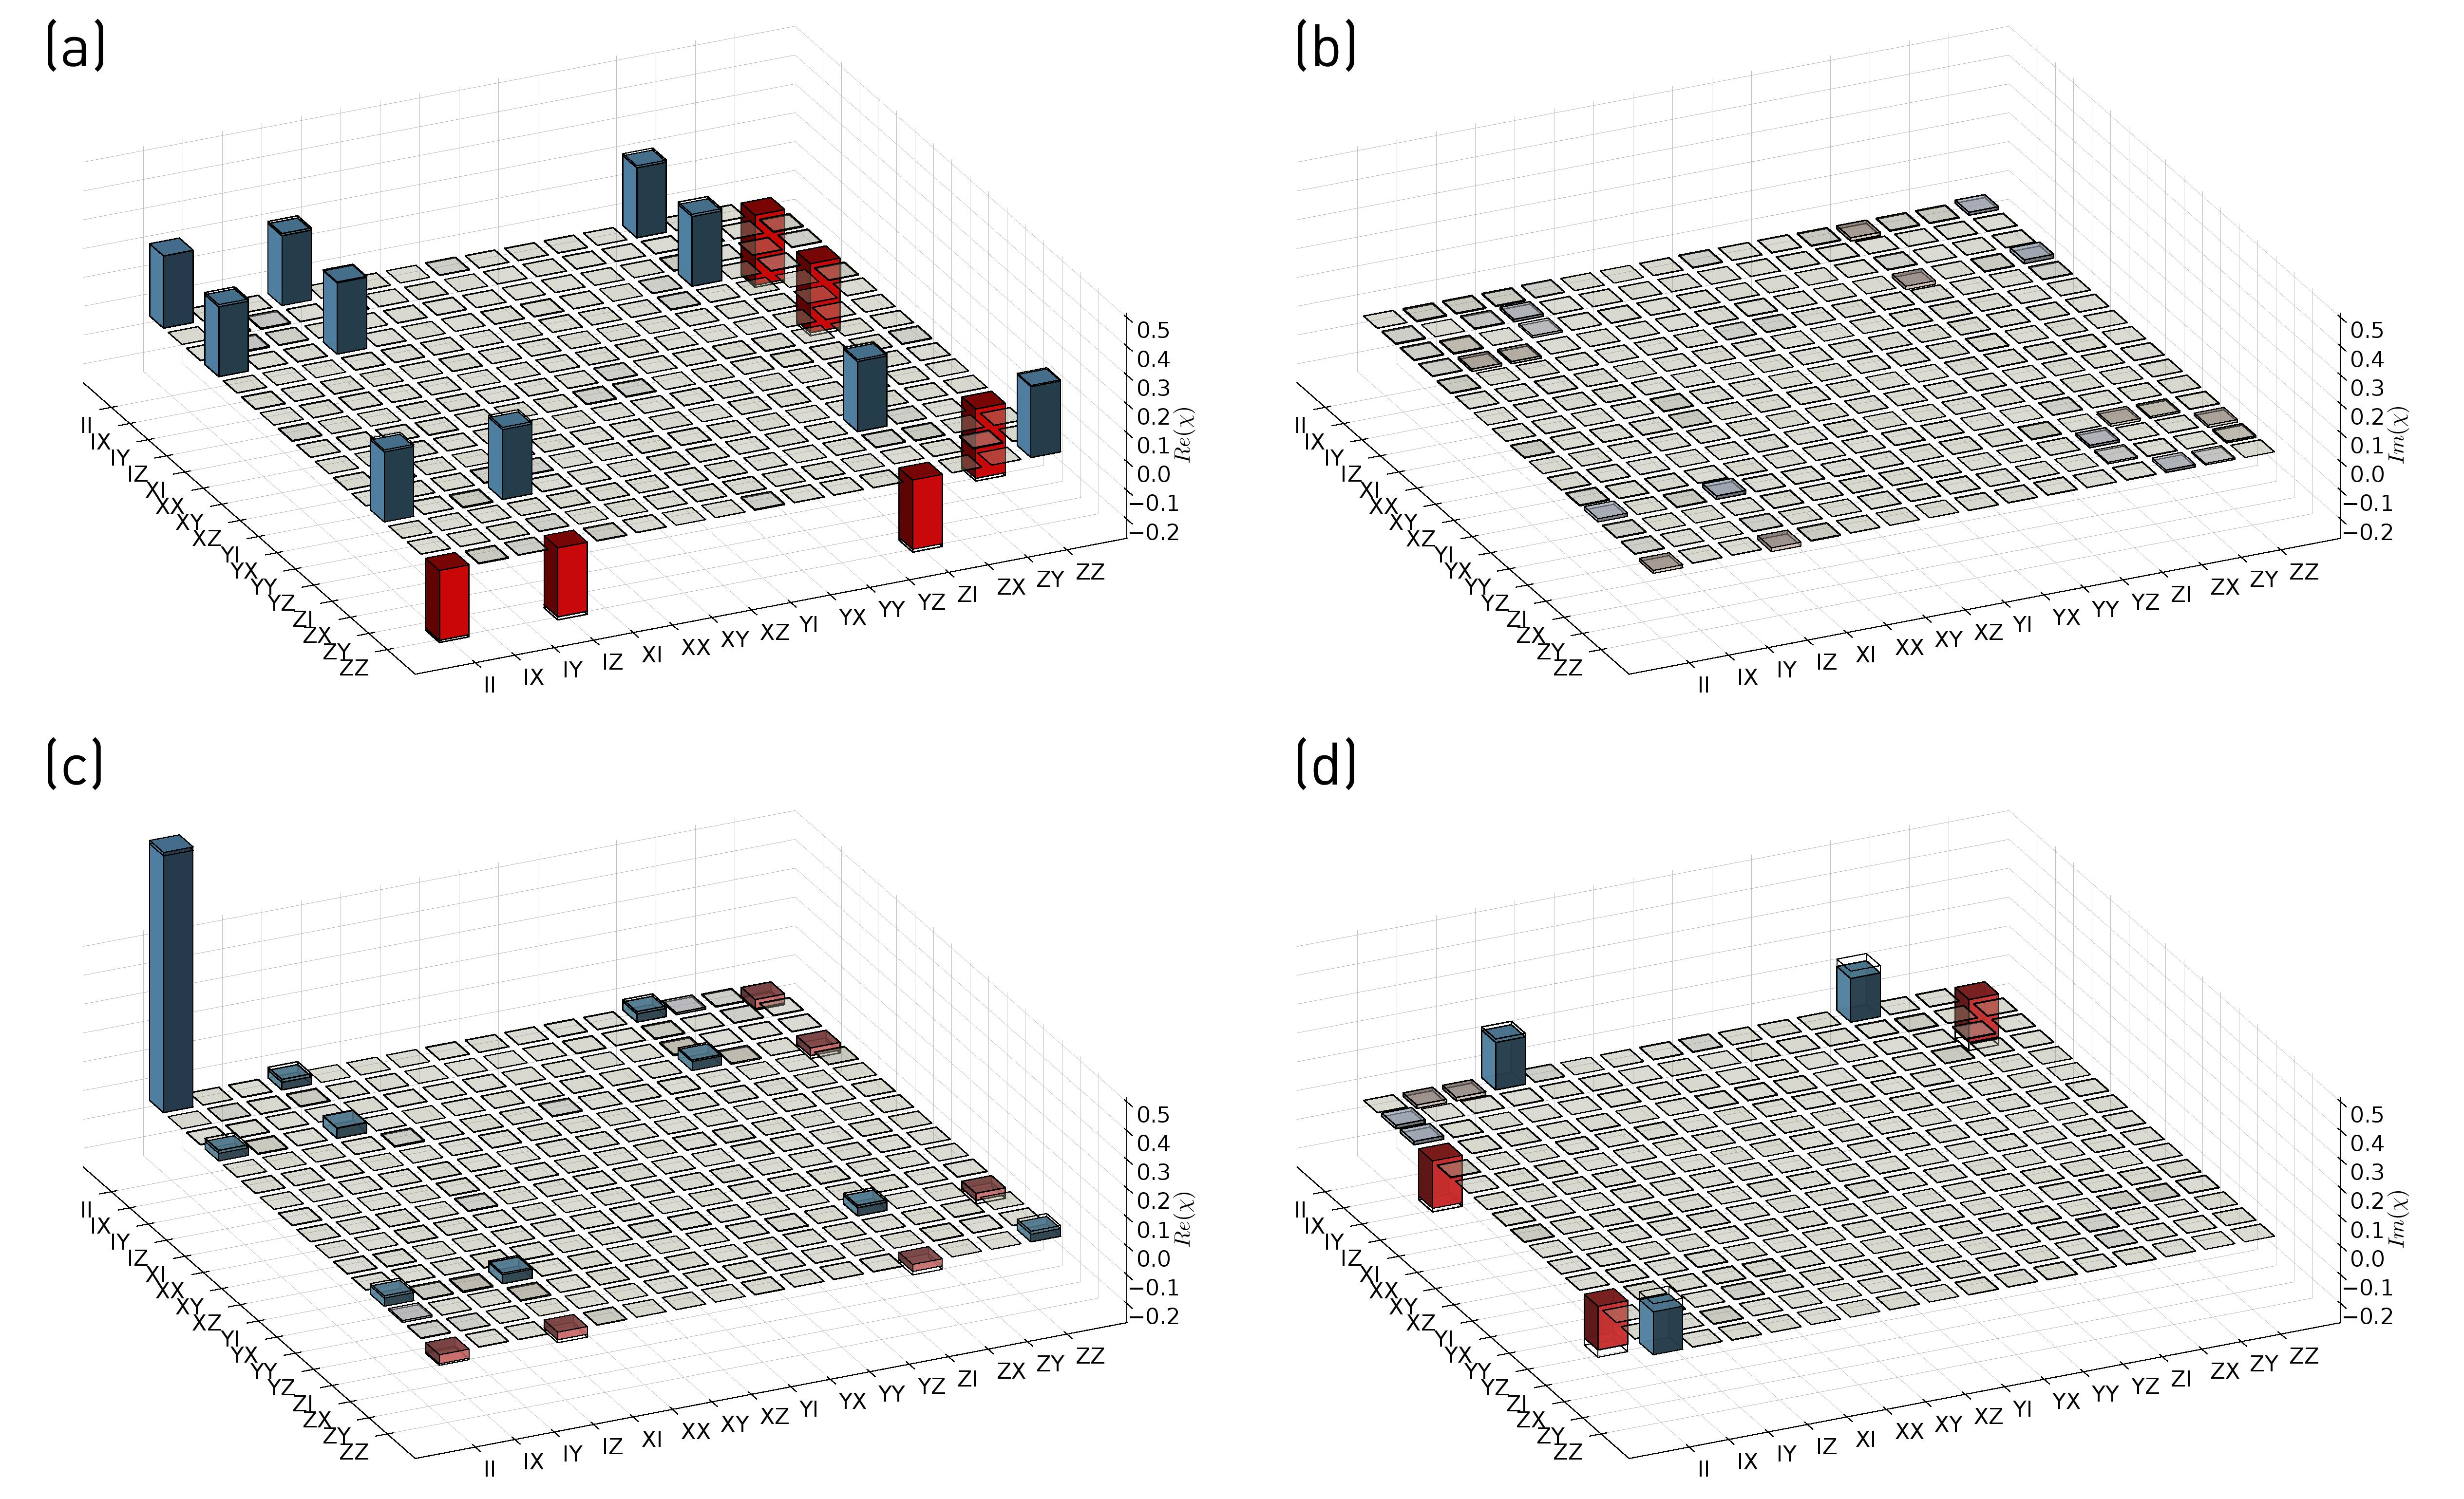
\includegraphics[width=\textwidth]{chapters/carb_gate/figs/process_tomography_chi_mtx.jpg}
    \caption{Real (a, c) and imaginary (b, d) elements of the process matrices $\chi^\pi$ and $\chi^{7\pi/4}$ respectively. The black wire frame corresponds to the target process matrix, while the blue (positive values) and red (negative values) filled bars correspond to the recontructed process matrix from measurements. The process fidelity for the phase  $\pi$ ($7\pi/4$) is 97.3\% (98.3\%).   }
    \label{fig:carb_characterization_chi_matrices}
\end{figure}

In Fig.~\ref{fig:carb_characterization_process_fidelity}, we show the process fidelity for 7 phase angles of the \gls{carb}. The maximum (minimum) fidelity is $98.3\%$ ($97.3\%$), for a phase of $7\pi/4$ ($\pi$). The expected fidelity from a master equation simulation including effects of decoherence during the gate is shown as dotted line. It explains about 1 \%, and is largest near phases of $\pi$. Thermal population  (0.4\% (1.3\%) at the time of the measurement on qubit 2 (3)) also affects the fidelity of the gate. Nevertheless, evaluating its effect precisely is not trivial: during \gls{qpt} the thermal population is mixed into other states with the tomography preparation pulses. Therefore, we scale the fidelity obtained by simulation by the probability that both qubits are in the ground state before starting the measurement. We suggest that this constitutes an approximate lower bound for the fidelity. This lower bound corresponds to the dashed line in Fig.~\ref{fig:carb_characterization_process_fidelity}. While this lower bound closely matches the measured fidelities near phases of $\pi$, it underestimates the fidelity for small and large phases. We expect this underestimation arises because both low and large conditional phase gates are closer to an identity operation and in the limit of a fully mixed (thermal) state, any gate behaves the identity operation. A detailed theoretical analysis is beyond the scope of this thesis (see e.g.~\cite{Korotkov2013ErrorTomography}).

\begin{figure}[ht]
    \centering
    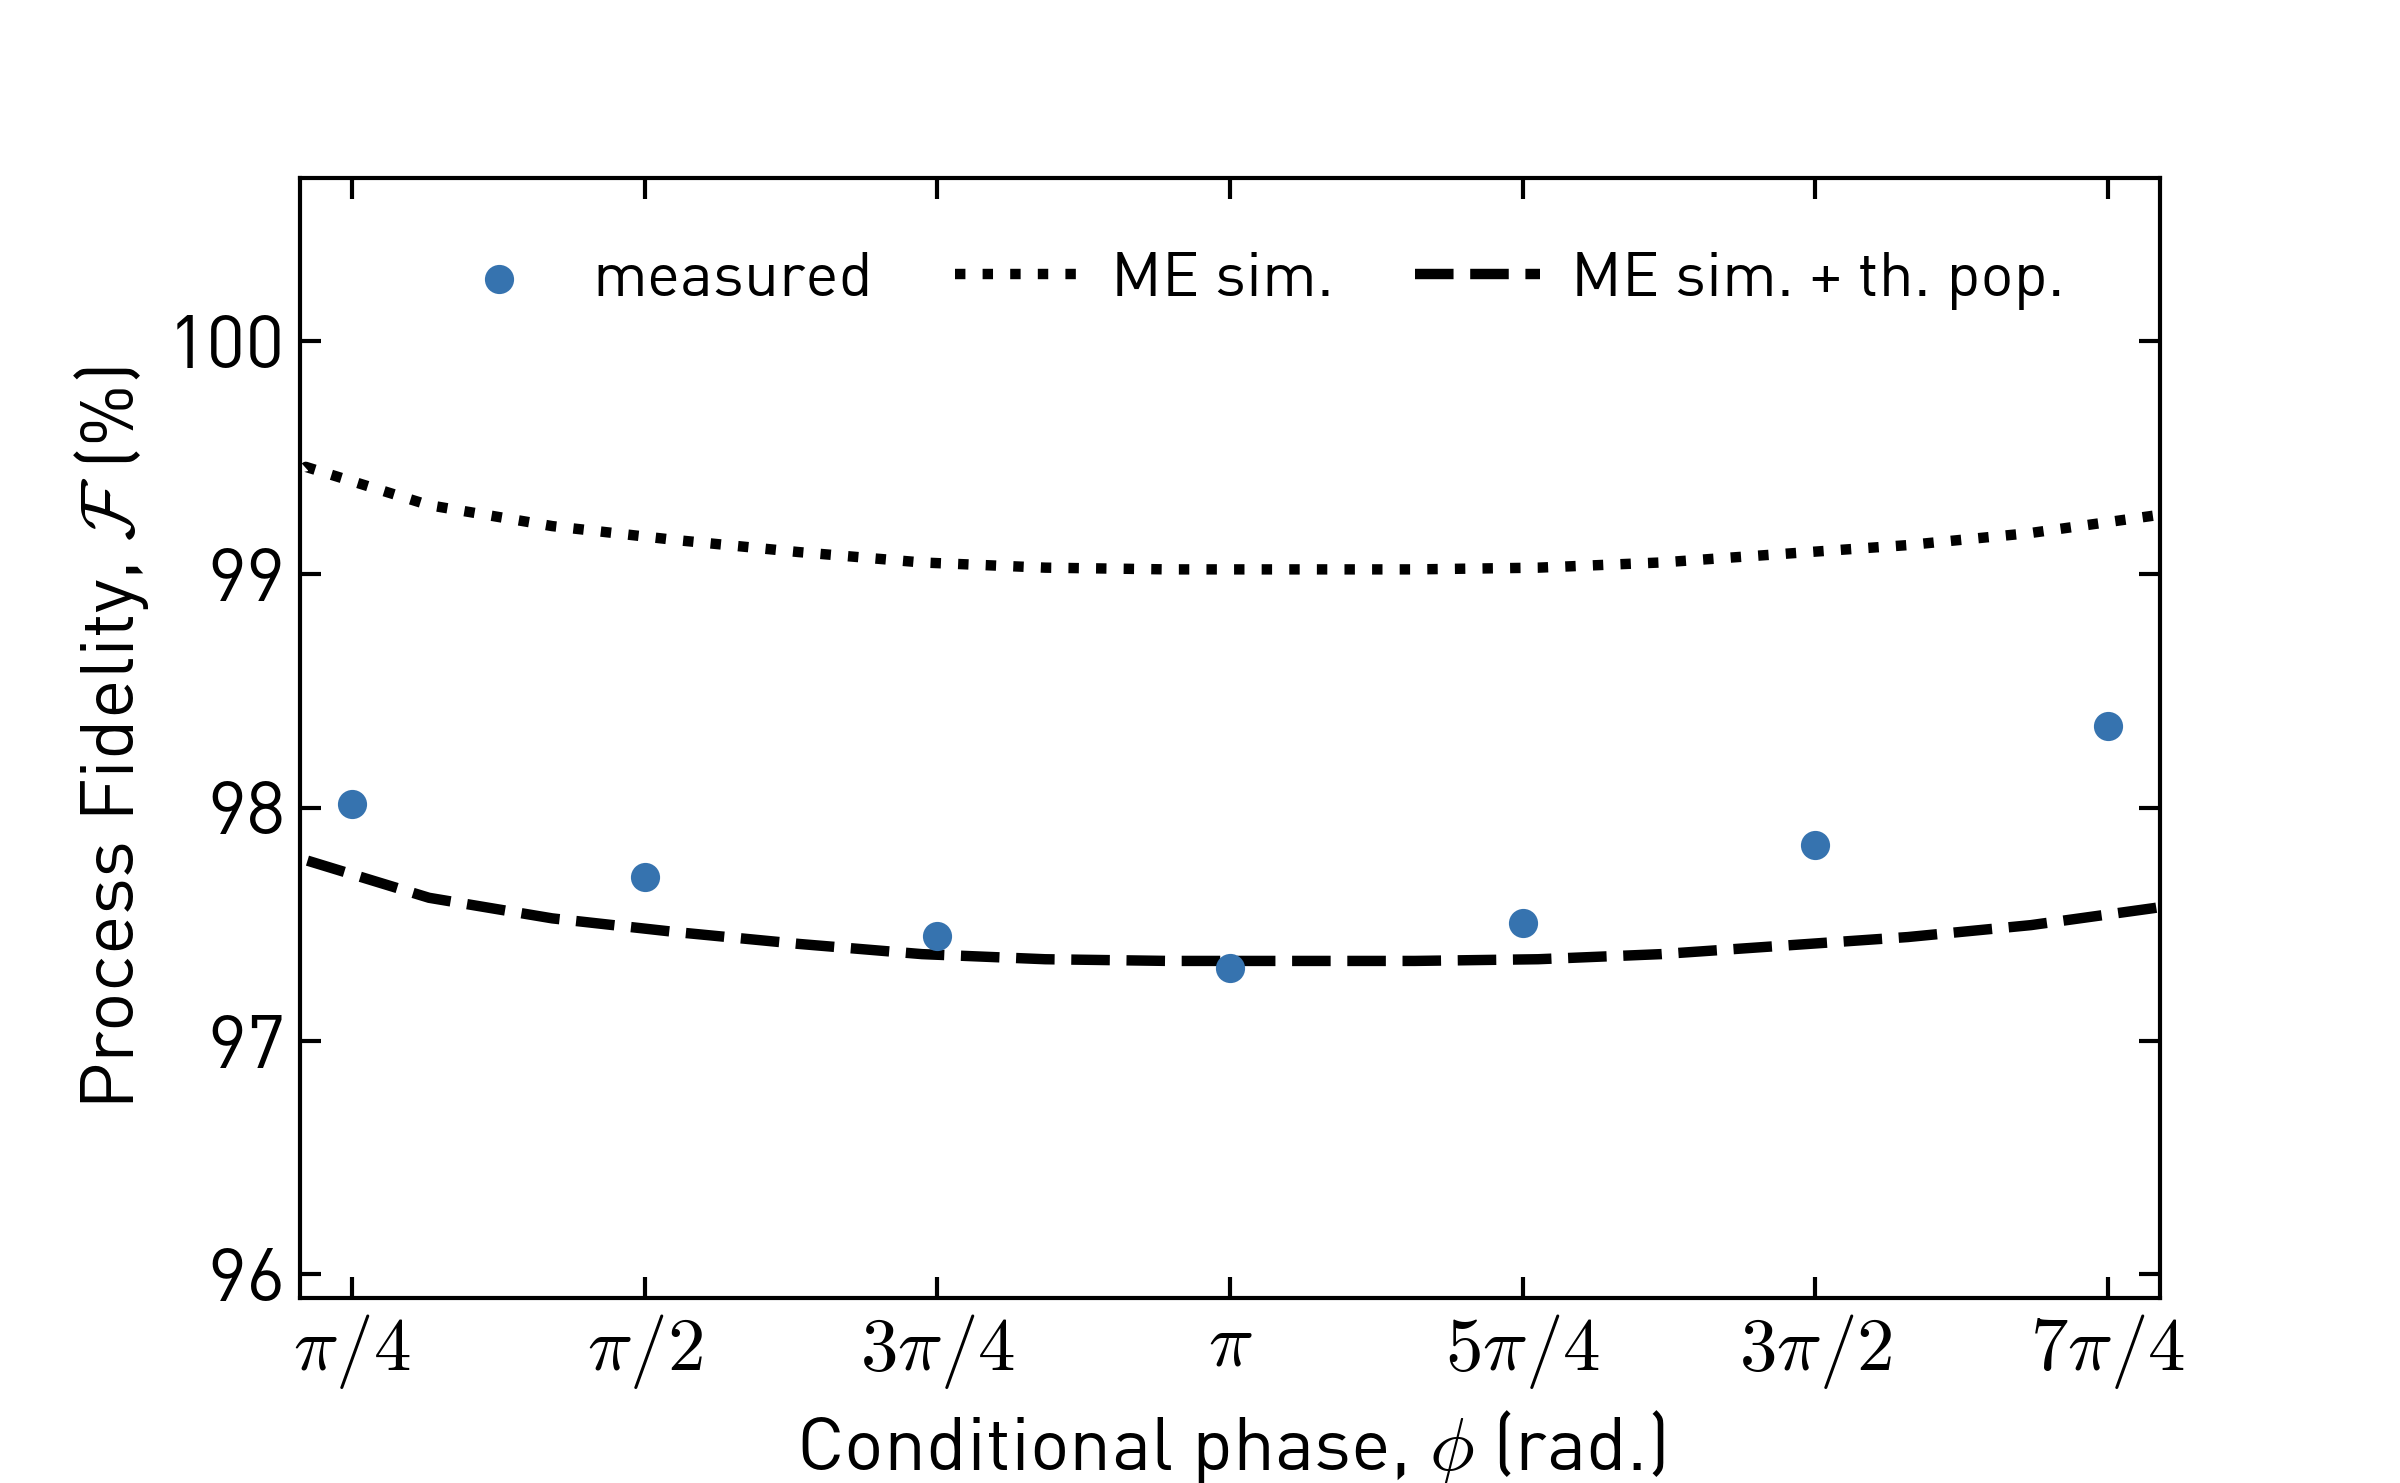
\includegraphics[width=\textwidth]{chapters/carb_gate/figs/ch4_characterization_tomo_all_angles_20200406_144758.png}
    \caption{Process fidelity as function of conditional phase angle of the \gls{carb}. Measurements are shown in scattered points.  Master equation simulation including effects of decoherence in dotted line. The dashed line corresponds to the fidelity of the simulation scaled by the probability of starting the measurement in the ground state. }
    \label{fig:carb_characterization_process_fidelity}
\end{figure}

Although \gls{qpt} yields full information of the quantum process, it also has several downsides. It is a time-consuming measurement and does not provide a direct and intuitive explanation about the different origin of errors. In addition, the maximum likelihood estimation of the process matrix relies on the assumption that state preparation and measurement errors are negligible, which is not necessarily the case when the length of the two-qubit pulse is on the same scale as the single-qubit tomography pulses (i.e. for small and large target conditional phases). Finally, it does not include information about leakage. We therefore perform additional characterization measurements in the next section which portray leakage and phase errors directly.

\subsection{Phases errors and leakage} \label{sec:carb_characterization_phase_errors_leakage}
A natural way to test the gate before its usage in an algorithm is to target a conditional phase and assess how close the measured conditional phase is from the target. When using 3-level readout, this measurement also characterizes, for each target phase, the \f{} level population of the qubit leaving the computational subspace (in this case, qubit 2). A similar approach allows to assess how well we are able to predict the dynamic phase the fluxed-qubit acquires.

We perform such a sweep over a target conditional phase in the range $[0\degree, 360\degree[$ with a spacing of 8\degree{} and present the results in Fig.~\ref{fig:carb_characterization_phase_errors_leakage}(a). The conditional (dynamic) phase error shows a distribution with mean and standard deviation of $0.23\pm0.97\degree$ ($-0.28\pm1.38\degree$) respectively. To reduce the phase error even further, we could investigate different interpolation strategies. However, we argue that these phase errors will not be the limiting factor when used in algorithms. Indeed, the fidelity\footnote{We use the  definition of fidelity between two pure states $\psi_{\rho}$ and $\psi_{\sigma}$ as the squared overlap between the amplitudes: $\mathcal{F} = \left|\left\langle\psi_{\rho} | \psi_{\sigma}\right\rangle\right|^{2}$~\cite{Jozsa1994FidelityStates}. We define the gate fidelity as by the fidelity between the state resulting for the ideal gate and the state resulting from the faulty gate implementation, minimized over all input
states~\cite{Reiner2018EffectsSystems}.} of a gate subjected to an over-rotation $\delta\phi$ degrades with $\cos^2{\delta\phi}$~\cite{Reiner2018EffectsSystems}. Therefore, for $\delta\phi = 2 \degree \approx 2\sigma_{\textrm{err}}$, the expected infidelity is on the order of $0.1\%$ ($0.2\%$ when adding both conditional and dynamic phase errors). By comparison, the effect of decoherence leads to a 5 times larger infidelity, and the 400\unit{kHz} residual $ZZ$-coupling for a duration of $100 \unit{ns}$ induces a phase error of 14.4\degree{} on the \oo{} state\footnote{Note that errors resulting from residual $ZZ$-coupling do not accumulate during the two-qubit gate but rather during single-qubit pulses and idle time because the calibration of the conditional phase includes the phase resulting from residual $ZZ$-coupling}. 

The leakage population shows an angular dependency. It is minimal ($P_f \approx 10^{-3}$) for conditional phases far from 180\degree, namely when the gate is short and the \oo{} and \tz{} states are off-resonant. By contrast, we observe leakage of up to $2\%$ when the \oo{} and \tz{} states are near resonance. At resonance, the population transfer is maximal, leading to a maximum in leakage population when assuming a fixed probability excitations being trapped in the \tz{} state. The dominant source of leakage are the short timescale distortions of the flux pulse~\cite{Rol2019Time-domainProcessor} which are not perfectly compensated by the \gls{fir} filters used for pre-distortion~\cite{Butscher2018ShapingFiltering}.  Leakage of qubit 3, which does not go into the \f{} level during the pulse, is on the order of $10^{-4}$ for all target conditional phases.

\begin{figure}[ht]
    \centering
    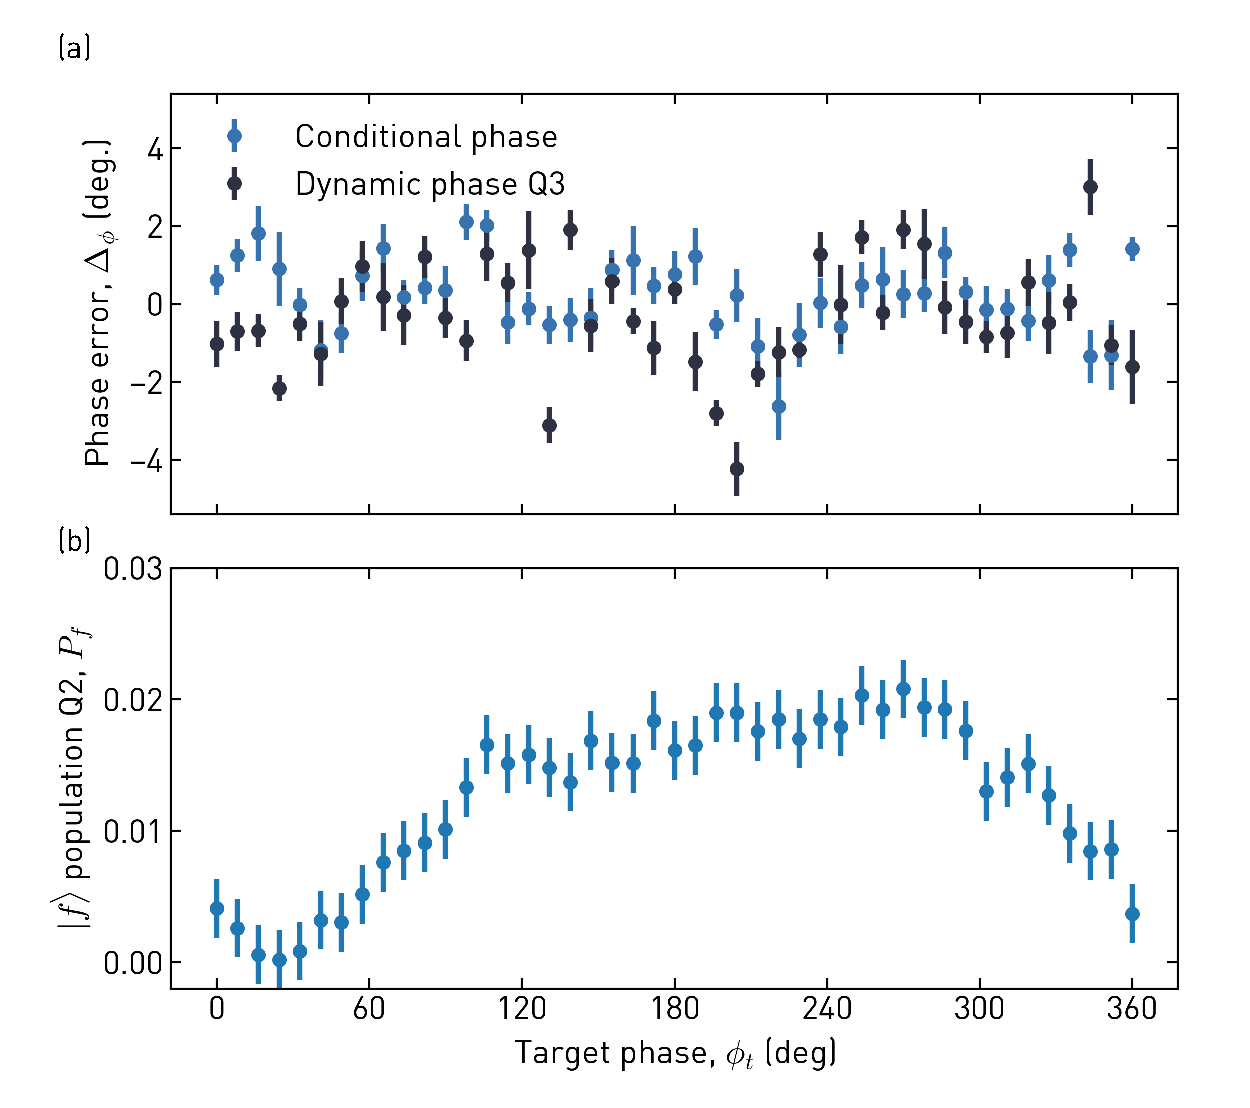
\includegraphics[width=\textwidth]{chapters/carb_gate/figs/ch4_characterization_phase_error_and_leakage_20200126_094856.pdf}
    \caption{Characterization of phase errors and leakage as function of target conditional phase with a granularity of 8\degree. Each point is averaged over 40000 single shots. (a) Conditional (light blue) and dynamic phase error (dark blue) show distributions with mean and standard distributions of $0.23\pm0.97\degree$ and  $-0.28\pm1.38\degree$ respectively. (b) We use 3-level readout to characterize leakage and measure up to 2\% leakage.}
    \label{fig:carb_characterization_phase_errors_leakage}
\end{figure}

\subsection{Comparison between C-ARB gates and CZ gates}
As final characterization procedure, we compare the \gls{carb} and \gls{cz} (implemented on the same qubits) in terms of phase errors, leakage and long term stability. We calibrate both gates and repeat the measurement described in Section~\ref{sec:carb_characterization_phase_errors_leakage}. For the \gls{cz}, we target a conditional phase of 180\degree, repeated $N$ times.  For the \gls{carb}, we sweep the range of target phases from 0 to 360\degree{} with $N$ points. These measurements are repeated for up to 15 hours after calibration. The full distributions of deviations from measured phases to target phases and leakages are presented as individual histograms, visualized as shaded filling in Fig.~\ref{fig:carb_characterization_drift}.

Both gates exhibit a similar range of conditional phase errors (standard deviation of $0.95\degree{}$ for the \gls{carb} versus $0.80\degree{}$ for the \gls{cz}). We conclude that extending the \gls{cz} to a \gls{carb} does not strongly impact the ability of preparing a target conditional phase. Note that the \gls{cz} shows a consistent offset of approximately 1\degree{} with respect to its target conditional phase. This originates from the fact that the gate is calibrated with a single point, which in this case was on the lower tail of the distribution. 

The \gls{carb} displays a wider distribution of dynamic phase errors, with an average standard deviation of 1.26\degree{} versus 0.83\degree{} for the \gls{cz}. This suggests it is harder to calibrate the dynamic phase for many flux pulse amplitudes and lengths simultaneously compared to calibrating only one. Preliminary analysis also suggest that the interpolation method has an influence on the standard deviation of the dynamic phase error. Using a cubic spline interpolation could help reduce the dynamic phase interpolation errors, compared to the implemented linear interpolation. 

The qubit 2 leakage trends are consistent with the discussion in Section~\ref{sec:carb_characterization_phase_errors_leakage}: the \gls{cz} experiences an average leakage of approximately 2\% since the \oo{} and \tz{} levels are on resonance. By contrast, the \gls{carb} experiences an average leakage of 1.4\% as several conditional phases result in low leakage. Its worse case leakage, however, is comparable to the one of the \gls{cz}. 

The phase error distributions stay relatively stable in time for both gates which suggests they will provide stable performance in algorithms for up to 15 hours after calibration.

The gates also differ in their average lengths. This effect is best visualized in Fig.~\ref{fig:ch4_calibration_carb}(a). While the \gls{cz} has a fixed flux pulse length of $107\unit{ns}$, the \gls{carb}'s flux pulse length is target phase dependent.  Averaged over all conditional phases, the flux pulse length is $84\unit{ns}$ long or $\sim 20\%$ shorter than for a conditional phase of 180 \degree. For both implementations, we add a $10\unit{ns}$ ($15\unit{ns}$) buffer at the start (end) to avoid overlap of other gates with the rising and falling edges of the flux pulse.

\begin{figure}[ht]
    \centering
    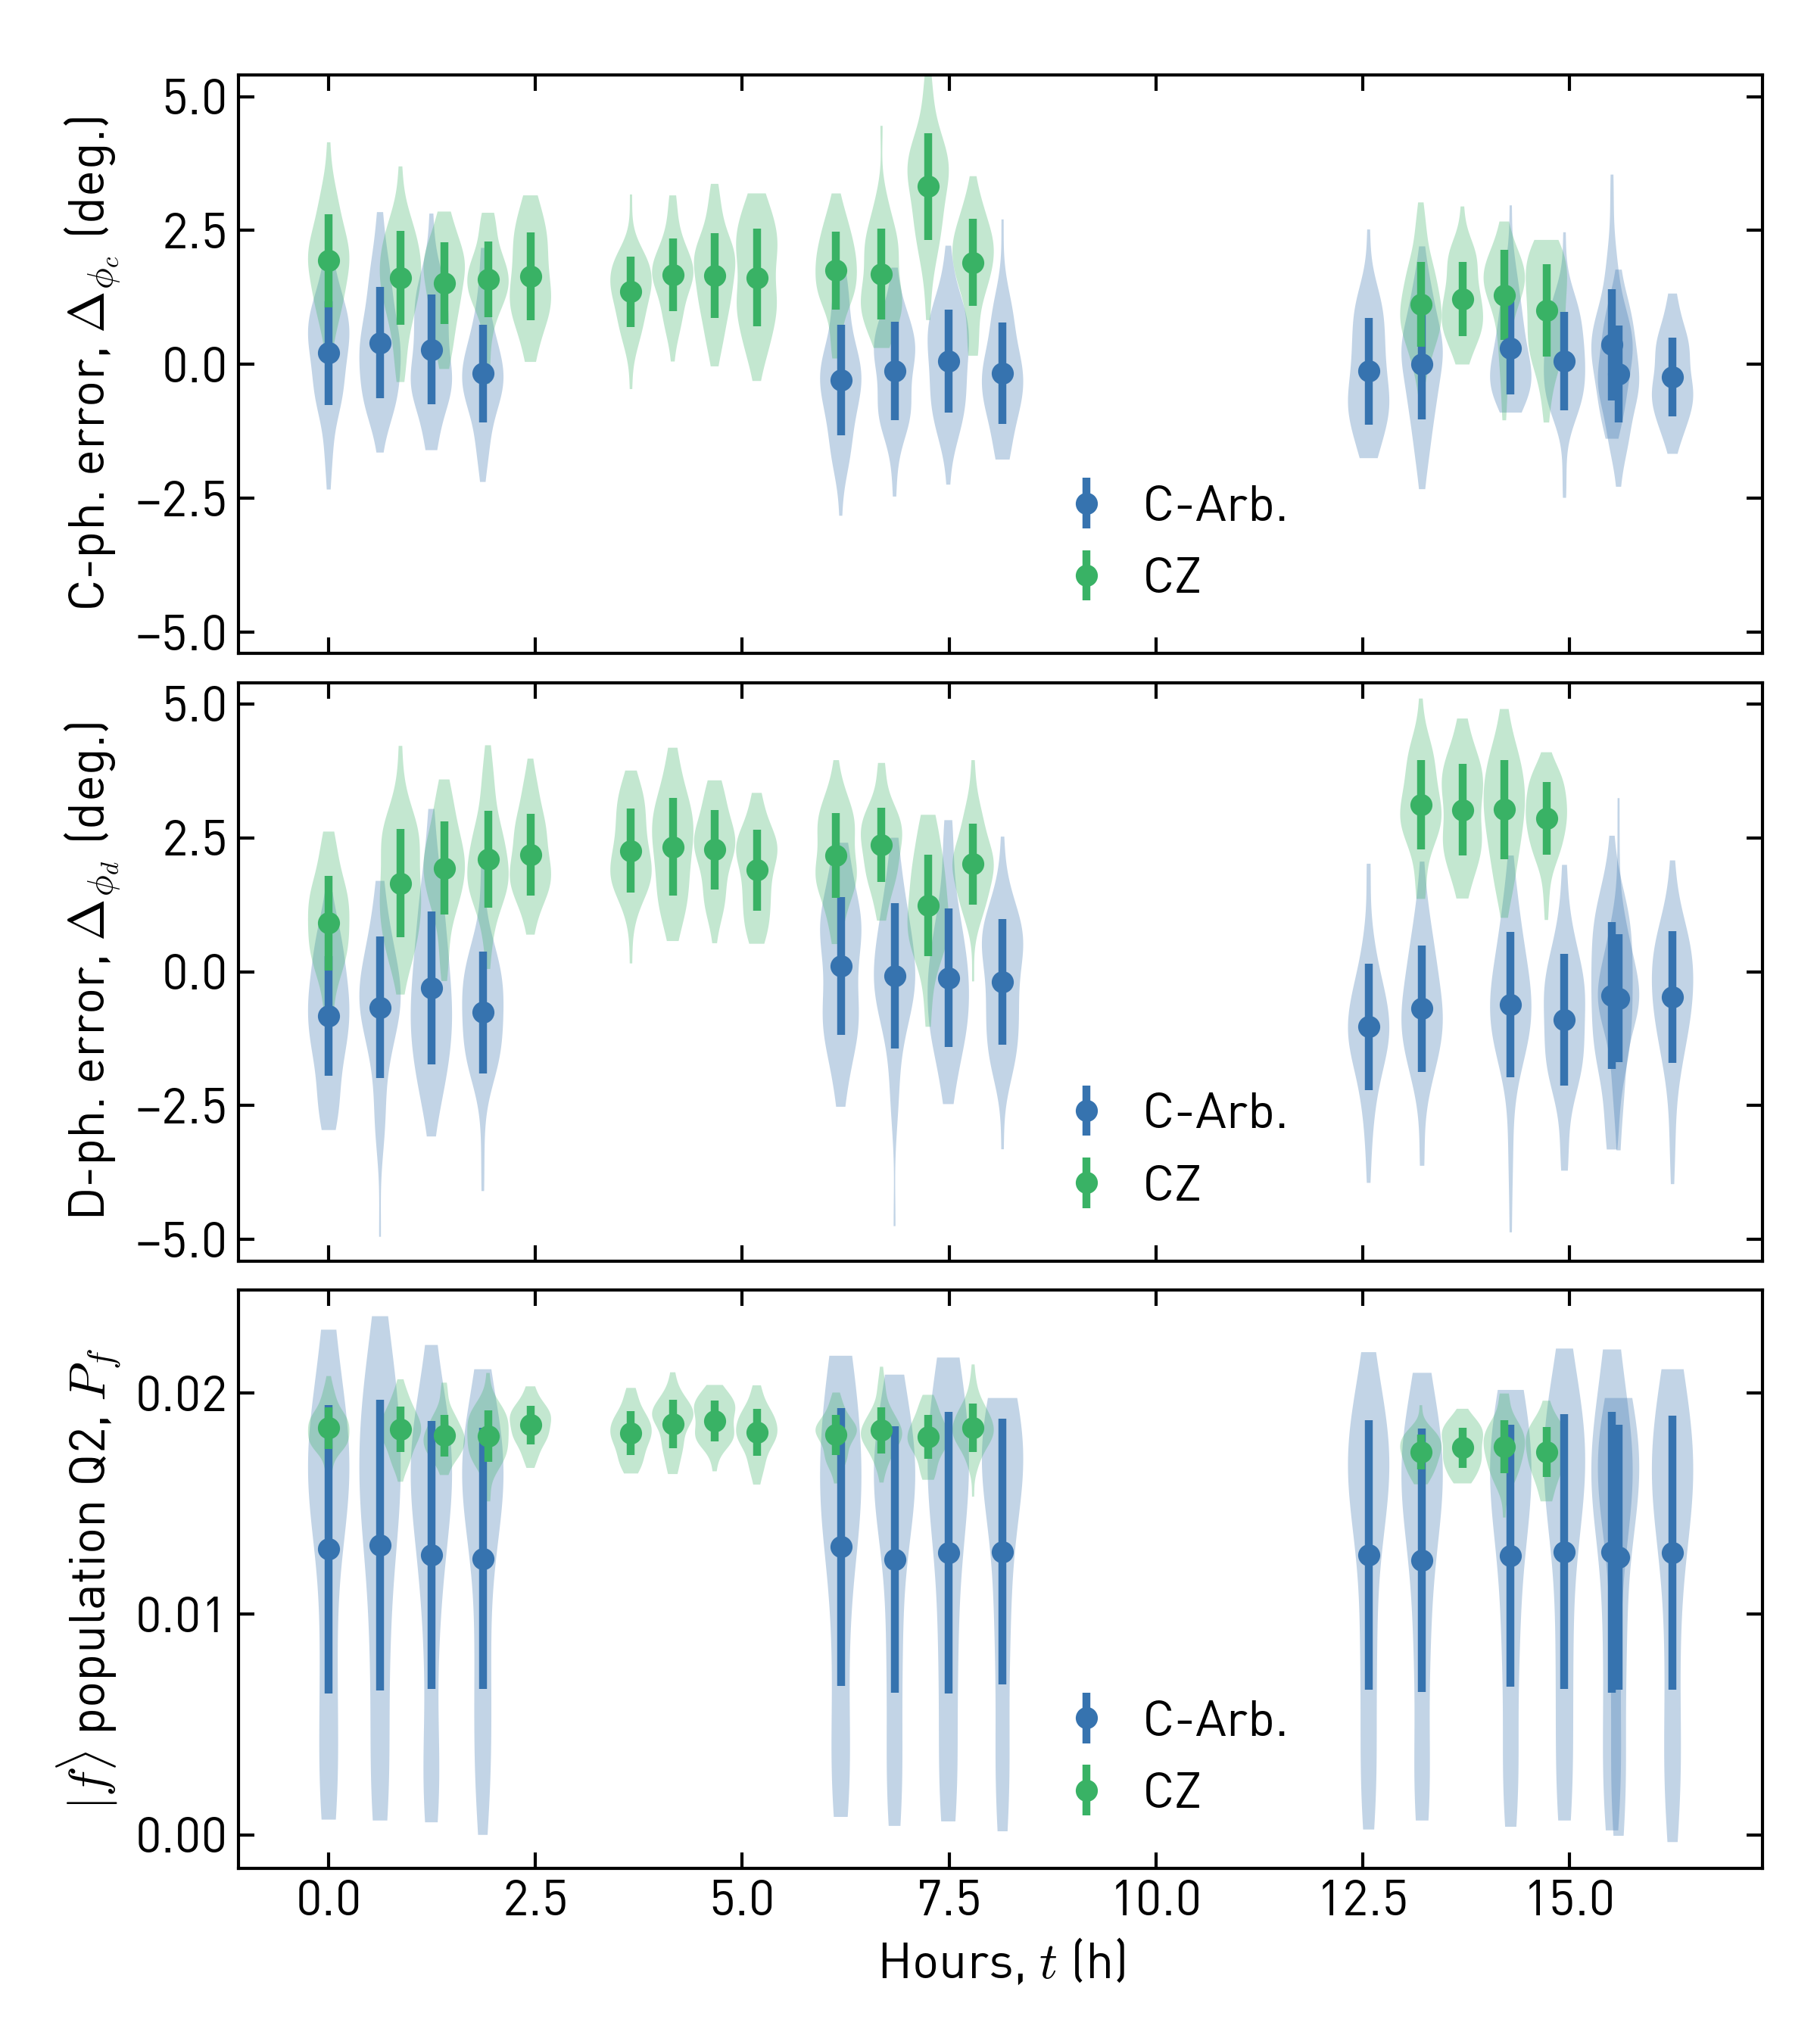
\includegraphics[width=\textwidth]{chapters/carb_gate/figs/ch4_characterization_drift_20200124_175455.png}
    \caption{Comparison between the \gls{cz} (green) and \gls{carb} (blue) in terms of phase errors and leakage as a function of time elapsed since calibration. The error bars correspond to the mean and standard deviation while the full distribution ($N$ = 45 points) is shown as shaded filling.}
    \label{fig:carb_characterization_drift}
\end{figure}

\section{Conclusion}
 In this chapter we have shown how to achieve a two-qubit unitary operation $U_{\textrm{C-ARB}}$ which adds an arbitrary phase $\phi$ on the \oo{} state. We implement this unitary by varying the frequency detuning between the \oo{} and the non-computational \tz{} state with a square,  Gaussian-filtered flux pulse. We adjust the length of the flux pulse to ensure high population recovery in the computational subspace. In practice, we calibrate the gate for a finite number of conditional phases (45) and interpolate linearly all parameters to reach phases between the calibration points. 
 
 We have characterized the gate using quantum process tomography for different conditional phases yielding a fidelity between 97.3\% and 98.3\%. The infidelity is dominated by decoherence and thermal population. In addition, we have shown that phase errors are small compared to other error mechanisms such as decoherence and residual $ZZ$-coupling. The average leakage amounts to 1.4\% and originates from the distortions of the flux pulse which are not corrected by the finite impulse response filter. The \gls{carb} shows similar time stability and phase error distributions as a \gls{cz} implemented on the same qubits while being 20\% shorter on average. 
 
 Although its calibration procedure is more elaborate, the \gls{carb} enables a significant gate count reduction for of \gls{vqa} circuits. In the next chapter, we implement a three-qubit problem instance which we solve using the \gls{qaoa} to demonstrate this advantage.



\chapter{Solving an exact cover problem instance using the QAOA} \label{ch:qaoa}
\glsreset{qaoa}
In this chapter, we first introduce combinatorial optimization. Next, we explain the \gls{qaoa}, a quantum heuristic algorithm providing approximate solutions to combinatorial optimization problems. We show that using \glspl{carb} can reduce the length of a \gls{qaoa}'s gate sequence implemented on the quantum computer. Next, we demonstrate this advantage experimentally by solving an exact cover problem instance on a three-qubit quantum processor.

\section{Combinatorial optimization}
An optimization problem for which the aim is to find the optimal (or close to optimal) solution amongst a finite set of possibilities is called a \textit{combinatorial optimization problem}.  Such problems are pervasive and appear in applications such as logistics, hardware verification, telecommunication network design, task scheduling and many more~\cite{Sbihi2007CombinatorialA, Coles2018QuantumBeginners, 2014ApplicationsOptimization}.

In its general form, a combinatorial optimization problem is specified by a set of rules, called clauses, acting on strings of $N$ bits, in which each bit represents a binary decision variable~\cite{Farhi2014AAlgorithm}.  Each clause is satisfied for certain assignments of the bits and unsatisfied for other assignments. Solving the problem consists in finding a combination of bits (forming together the bit string, $b := b_1 \, ...\, b_N$) satisfying the largest (weighted) amount of clauses. The objective function can be written as 
\begin{equation} \label{eq:qaoa_clauses}
    C(b) = \sum_{m=1}^M w_m C_m(b)
\end{equation}
where $C_m(b)$ is the $m$-th clause and $w_m$ is its corresponding (real and non-negative) weight. If $C_m(b)$ is satisfied by the bit string $b$ then its value is 1 and otherwise 0. In these terms, solving the problem is expressed as finding the bit string $b_\text{opt}$ maximizing $C$. An approximate solution provides a bit string $b_{\text{approx}}$ for which  $C(b_{\text{approx}})$ is close to the maximum of $C$.

We illustrate this abstract concept with a simple example. Imagine you  have to choose an outfit -- consisting of one t-shirt and one pair of pants -- from your closet. You have 2 shirts to choose from, a white and blue one. Similarly, you have a white and a blue pair of pants. You believe you look better when your whole outfit is of the same color. Additionally, you think your blue shirt suits you better than the white one. Which outfit should you choose for the party? 

While the answer is trivial in this example, we formalize the problem with the terminology introduced above. The outfit, $b = b_1b_2 $, can be formulated as a 2-bit string, one bit for the shirt ($b_1$), and one for the pair of pants ($b_2$). Colors are encoded by the values of the bits: 0 for white and 1 for blue. The four possible outfits are: 00 (white-white), 01 (white-blue), 10 (blue-white) and 11 (blue-blue). The problem has two clauses. $C_1(b) = \neg (b_1 \oplus b_2)$, leading to a value of 1 if you choose a shirt and pair of pants of the same color and 0 otherwise\footnote{$\oplus$ denotes the "XOR" operation and $\neg$ is the logical not.}. $C_2(b) = b_1$ has a value of 1 only if you decide on wearing your blue shirt. The objective function is then:
\begin{equation}
    C(b) = C_1(b) + C_2(b) = \neg (b_1 \oplus b_2) + b_1
\end{equation}
where we assigned equal weights $w_1 = w_2 = 1$ to both clauses.
The score of each output is then:
\begin{subequations}
\begin{equation}
     C(00) = 1 + 0 = 1
\end{equation}
\begin{equation}
    C(01) = 0 + 0 = 0
\end{equation}
  \begin{equation}
      C(10) = 0 +  1 = 1
  \end{equation}
  \begin{equation}
         C(11) = 1 + 1 = 2
  \end{equation}
\end{subequations}

The bit string maximizing $C(b)$ is indeed 11 (blue shirt, blue pants). An algorithm capable of providing this bit string is a combinatorial optimization algorithm. In this case, we used the exhaustive search algorithm, meaning that we enumerated all possible answers and picked the best one. 

In many real applications, exhaustive search is not tractable. In fact, even a slight modification of the presented problem makes it unrealistic to use exhaustive search. Instead of 2, imagine having to choose 25 items, each available in 8 different colors (each item has now 3 bits to encode the colors). The number of possible outfits becomes $2^{3 \cdot 25} \approx 4\cdot 10^{22}$. It would take about a million years to search sequentially through all possibilities for a computer requiring $1\unit{ns}$ to evaluate the cost of each outfit\footnote{Note that you are confronted to a similar situation every morning when dressing up. But you do not use the exhaustive search algorithm to decide what you wear, otherwise you would never get out of your house.}.

Several (classical) heuristic algorithms exist providing an approximate solution for this type of problems. In the next section, we explain the \gls{qaoa}, a quantum heuristic algorithm capable of finding approximate solutions to this type of problems.

\section{The quantum approximate optimization algorithm}\label{sec:qaoa}
The \gls{qaoa}~\cite{Farhi2014AAlgorithm} (depicted in Fig.~\ref{fig:qaoa_scheme}(a)) is a \gls{vqa} designed to find approximate solutions to combinatorial optimization problems. It is a hybrid algorithm executed partially on a quantum computer and partially on a classical computer. 

First, the quantum computer prepares a quantum state $\ket{\vec{\gamma}, \vec{\beta}}$ based on the objective function\footnote{Also often named cost function in the context of a minimization problem.} $C$ characterizing the clauses of the problem (see Eq.~\eqref{eq:qaoa_clauses}), and a set of variational parameters $\theta = (\vec \gamma, \vec \beta)$. The state is prepared with $p$ layers of two unitaries corresponding to the time-evolution of two non-commuting Hamitltonians, $\hat C$ and $\hat B$, applied to a uniform superposition state of $N$ qubits,
\begin{equation}
    |\vec{\gamma}, \vec{\beta}\rangle=\underbrace{\sexp{-\i \beta_{p} \hat B} \sexp{-\i \gamma_{p} \hat C}}_{\text {layer } p} \cdots \underbrace{\sexp{-\i \beta_{1} \hat B} \sexp{-\i \gamma_{1} \hat C}}_{\text {layer } 1}|+\rangle^{\otimes N}
\end{equation}
where  $\ket{+}^{\otimes N} = \left(\frac{1}{\sqrt{2}}(\ket{0}+\ket{1})\right)^{\otimes N}$ is the initialization state, and $\vec\gamma = (\gamma_1, ..., \gamma_p)^\text{T}$ and $\vec\beta = (\beta_1, ... , \beta_p)^\text{T}$ are the real variational parameters for the $p$ layers. Referring to the number of layers, we say that the implementation is of depth $p$. $\hat C$ is the cost Hamiltonian, which for all objective functions of NP-complete problems can be mapped to an Ising Hamiltonian in polynomial time~\cite{Lucas2014IsingProblems},
\begin{equation} \label{eq:ising}
    \hat C =\sum_{n < m} J_{n m} \sigma_{n}^z \sigma_{m}^z + \sum_{n} h_n \sigma_{n}^z
\end{equation}
and $\hat B$ is the mixing Hamiltonian 
\begin{equation}
    \hat B = \sum_{n} \sigma_n^x
\end{equation}
where $\sigma_n^{z}$ ($\sigma_n^{x}$) are the Pauli Z (X) operators applied to the $n$-th qubit, and $h_n$ and $J_{n m}$ are real coefficients. In the combinatorial optimization picture, these coefficients represent the relative weights of each clause, see Eq.~\eqref{eq:qaoa_clauses}.

\begin{figure}[H]
    \centering
    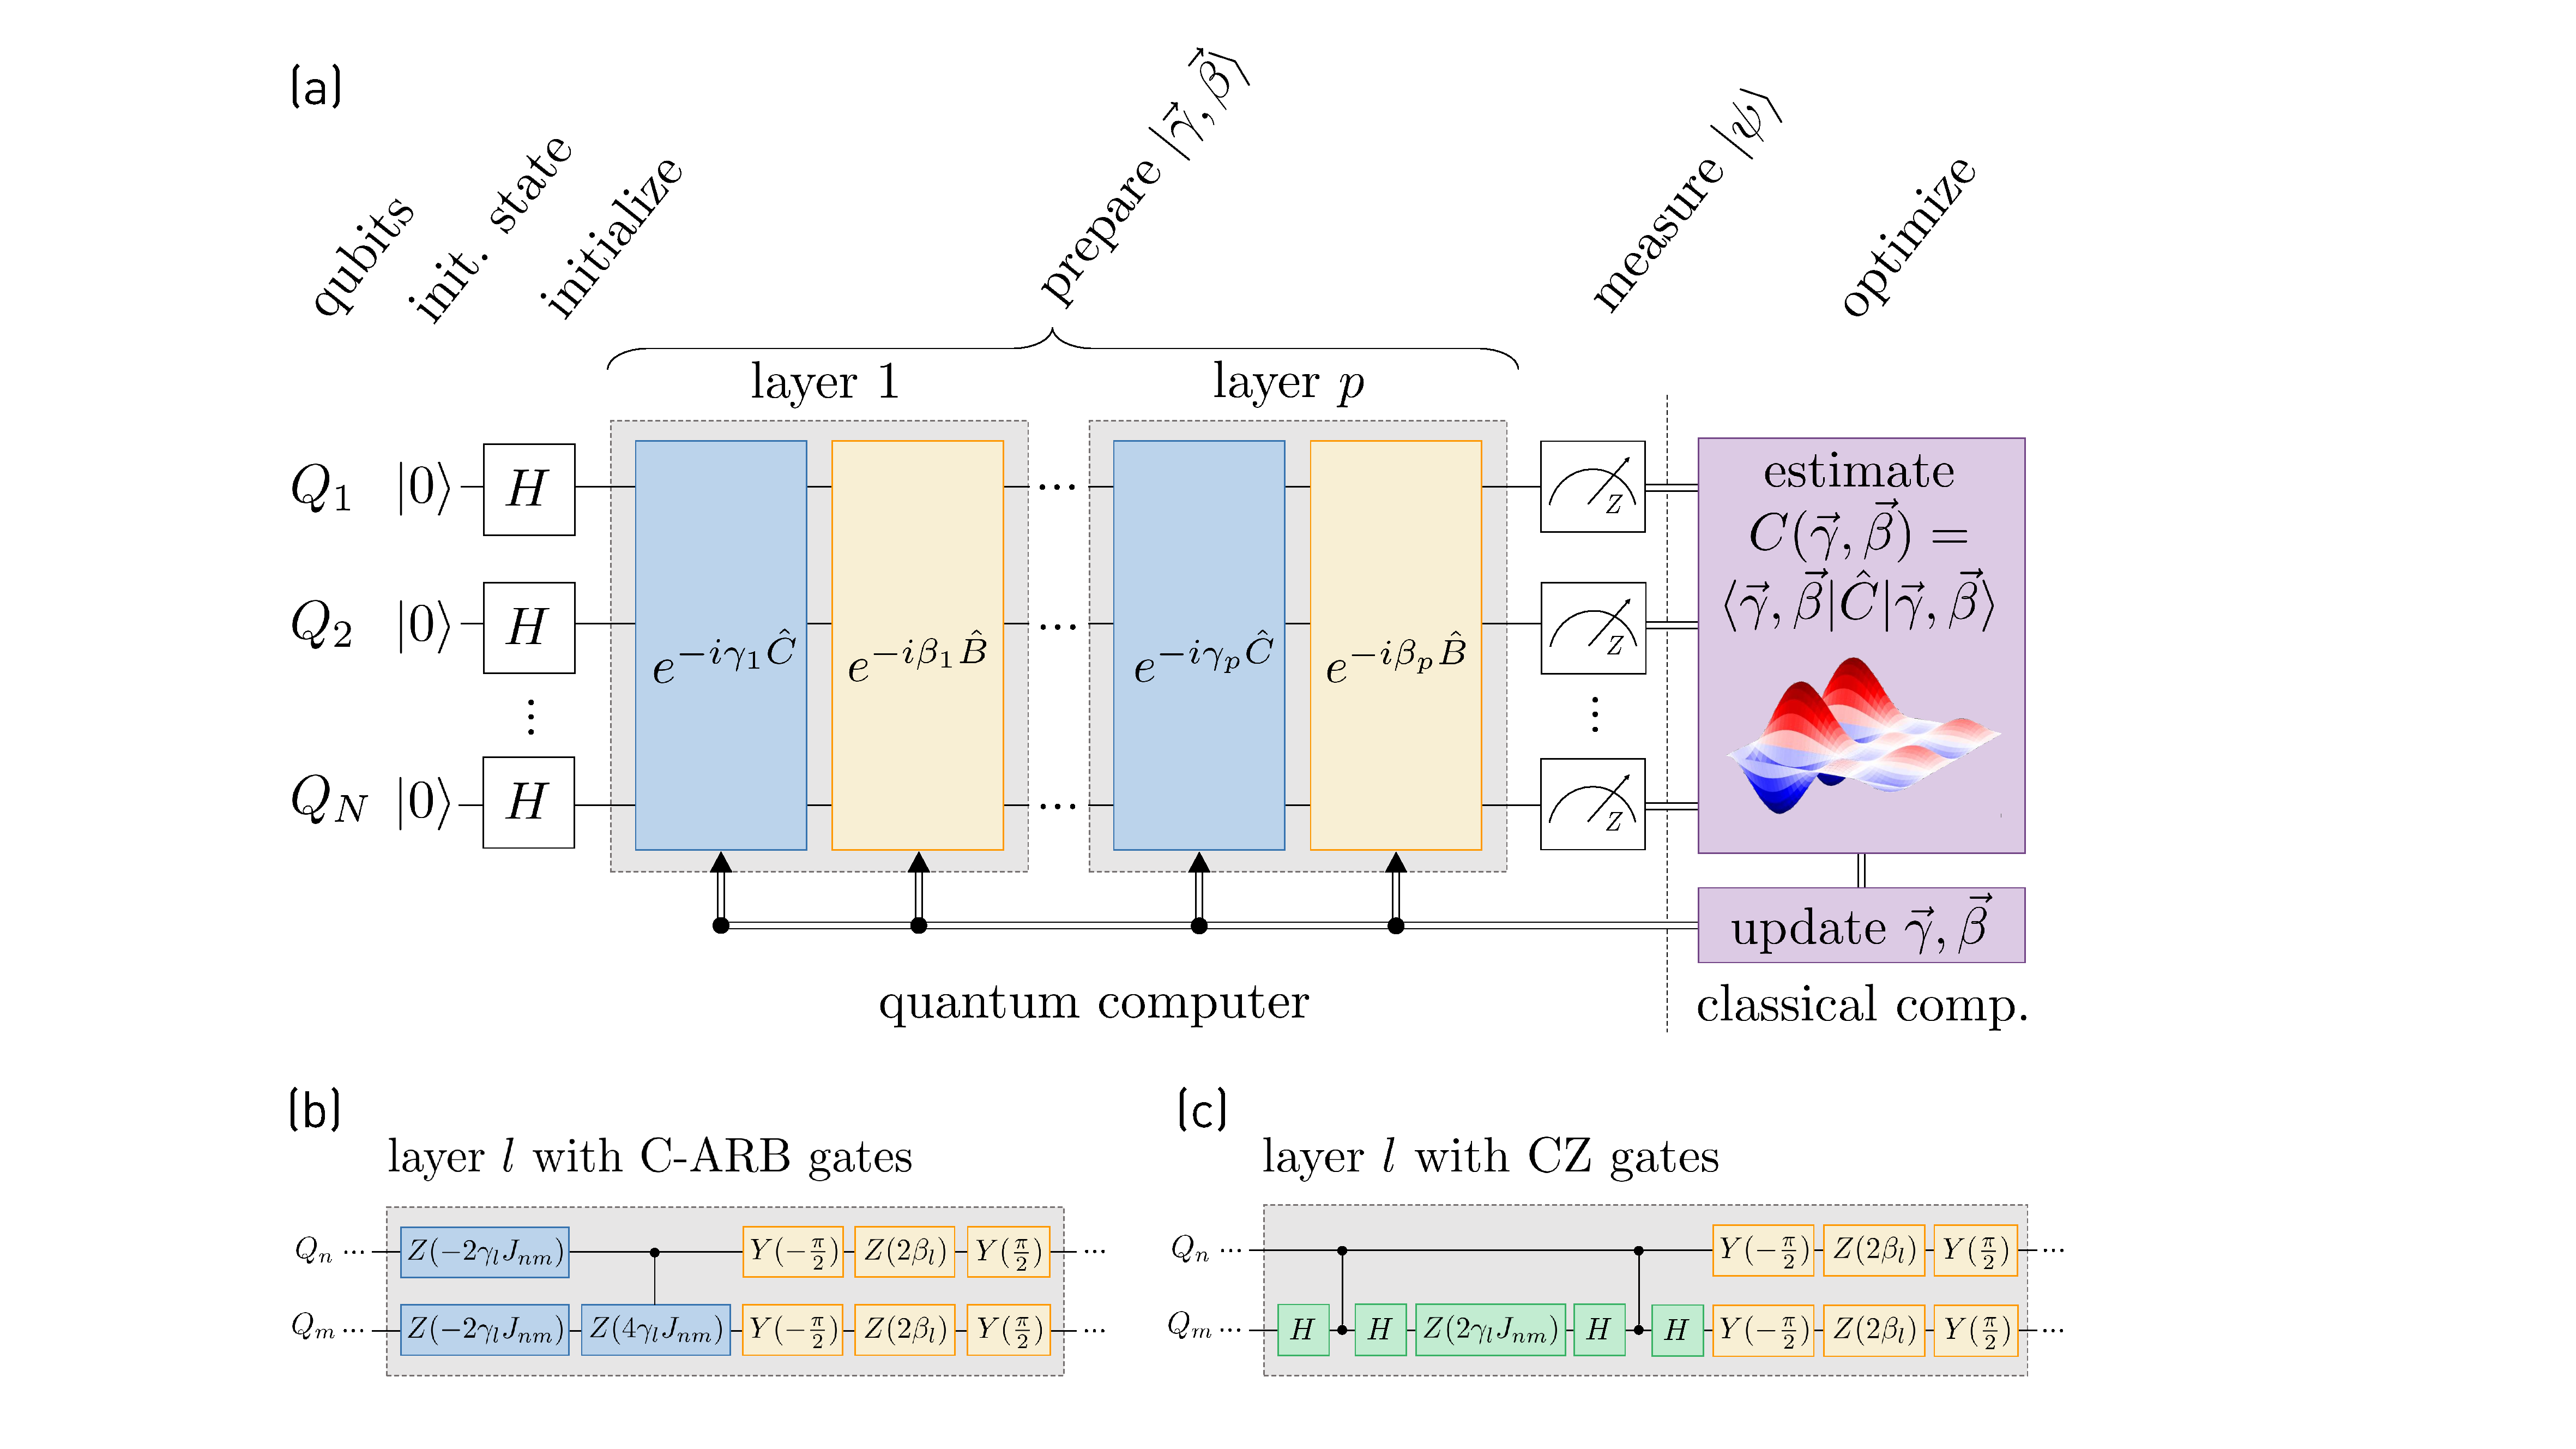
\includegraphics[width=\textwidth, trim ={9cm, 0 15cm, 0}]{chapters/qaoa/figs/qaoa_scheme-v6.pdf}
    \caption{The \gls{qaoa} scheme. $Z(\cdot)$ and $Y(\cdot)$ correspond to single-qubit z- and y-rotations while $H$ is the Hadamard gate. (a) The scheme consists of two steps. First, the quantum computer applies $p$ alternating sequences -- called layers -- of two unitaries corresponding to the time evolution of two Hamiltonians $\hat C$ (blue), $\hat B$ (yellow) scaled by layer-dependent variational parameters to an equal superposition state. The resulting state, \qaoaMeasuredState, is prepared and measured several times to obtain an estimate for the expectation value of a cost function \cost{}, based on the expectation values of single and two-qubit terms. Based on this estimate, a classical optimizer alters the variational parameters to minimize \cost{}. The output of the algorithm is the projection in the z-basis of state \optimalstate{} yielding a bit-string with a low cost. (b) Implementation of a layer of the \gls{qaoa} for a cost Hamiltonian consisting only of two-qubit interaction terms. Only two generic qubits, $Q_n$ and $Q_m$, are represented. The gate's background color indicates which part in (a) it implements. The single-qubit Z gates are virtual gates implemented by adding phase on the subsequent pulses. The two-qubit interaction is mediated by a \gls{carb}. The arbitrary single-qubit x-rotations are not calibrated on the device and are thus decomposed into two y-rotations and a z-rotation. (c) Equivalent gate sequence diagram as in (b) but featuring a decomposition of the \gls{carb} into \glspl{cz} and single-qubit gates.}
    \label{fig:qaoa_scheme}
\end{figure}

The resulting state \qaoaMeasuredState{} is measured in the $Z$ basis. A classical computer uses the measurement outcome (i.e.\ bit strings corresponding to the eigenstates of \qaoaMeasuredState{}) to compute the expectation value of $\hat C$ and iteratively updates the variational angles to optimize the objective function. When the objective function is mapped to the Ising Hamiltonian, the resulting problem consists in finding the lowest energy state of the system, i.e.\ minimizing the expectation value of the cost Hamiltonian. Once the optimizer has converged, the state \optimalstate{} constitutes an approximate solution for the optimization problem.

\subsection{Success probability} \label{sec:qaoa_success_prob}
Measuring successive preparations of \optimalstate{} yields a distribution on the eigenstates $\ket{\psi_i}$.
We define the success probability, $P_s$, as the probability of measuring an eigenstate that is a solution to the combinatorial problem. 

Note that the optimization is performed on the smooth landscape of the objective function \cost{} and not on $P_s$ directly. But for problems with a discrete domain of real values, a low expectation value of the cost function generally guarantees a high concentration of probability on optimal solutions upon measurement~\cite{Cook2019TheCover, Wang2019XY-mixers:QAOA}.

\subsection{Layer implementation}
The algorithm is subdivided into layers, in which each layer $l$ includes the unitary $\sexp{-\i\gamma_l\hat C}$. Since $\hat C$ is diagonal in the computational basis, all its terms commute. In addition, in this thesis we consider the case where all $h_n = 0$. Therefore, we look at the implementation of a single generic term $J_{nm}\sigma_n^z\sigma_m^z$ involving qubit $Q_n$ and qubit $Q_m$. Any other term in $\hat C$ can be applied before or after in the exact same way. 

The corresponding unitary to implement is $\sexp{-\i J_{nm} \gamma_l \sigma_n^z\sigma_m^z}$, yielding in the $nm$-two-qubit subspace,
\begin{equation} \label{eq:qaoa_two_qubit_cost_unitary}
    U_{nm}^l = 
    \begin{pmatrix}
    \sexp{-\i\gamma_l J_{nm}} & 0 & 0 & 0\\
    0 & \sexp{\i\gamma_l J_{nm}} & 0 & 0 \\
    0 & 0 & \sexp{\i\gamma_l J_{nm}} & 0 \\
    0 & 0 & 0 & \sexp{-\i\gamma_l J_{nm}}
    \end{pmatrix}
\end{equation}{}
We present two approaches to implement this unitary. The first one, which we call the \textit{\gls{dir}}, implements Eq.~\eqref{eq:qaoa_two_qubit_cost_unitary} with a single \gls{carb} and two single-qubit $Z$-gates (see Fig.~\ref{fig:qaoa_scheme}(b)). The \gls{carb} introduces a phase of $4\gamma_l J_{nm}$ on the \oo{} state which is then redistributed to the other diagonal terms by single-qubit $Z$-gates rotating their respective qubit subspace in the opposite direction with half the angle, i.e.\ $2\gamma_l J_{nm}$. Up to a global phase, this implements Eq.~\eqref{eq:qaoa_two_qubit_cost_unitary}. Note that, due to the presence of the variational parameter $\gamma_l$, the angle on the \oo{} state may have any real value and therefore indeed requires a \gls{carb} to rotate the \oo{} state with a single gate.

In case we choose to limit the gate set to the use of \glspl{cz} only (i.e.\ rotation of $\pi$ on the \oo{} state), we use a \textit{\gls{dec} } consisting of two \glspl{cz} and additional single-qubit gates (see green colored elements in Fig.~\ref{fig:qaoa_scheme}(c)).

In Section~\ref{sec:qaoa_experiment}, we compare experimentally the performance of both implementations.

\subsection{Relation to adiabatic quantum computing}\label{sec:qaoa_relation_to_adiabiatic_computing}
The depth $p$ of a \gls{qaoa} implementation is defined as the number of layers used for the state preparation. This parameter plays an important role both in theory and in experiments.

For $p \rightarrow \infty$, the \gls{qaoa} finds the global optimium of $C$~\cite{Farhi2014AAlgorithm}. Intuitively, this is because the \gls{qaoa} can be seen as a Trotterized approximation~\cite{TrotterMathematics} of the quantum adiabatic algorithm~\cite{Farhi2000QuantumEvolution}. Similarly to the \gls{qaoa}, the quantum adiabatic algorithm starts in the lowest energy state of the mixing Hamiltonian $\hat B$, i.e.\ the equal superposition over all qubits in the $Z$ basis, and then evolves adiabatically to the lowest eigenstate of the cost Hamiltonian $\hat C$. The time-dependent Hamiltonian during this evolution is

\begin{equation} \label{eq:qaoa_adiabatic_evolution}
 \hat H(t)=\hat H_1(t) +\, \hat H_2(t) = (1-t / T) \hat B + \, (t / T) \hat C
 \end{equation}
where $T$ is a real and positive parameter called run time. As long as the evolution is sufficiently slow i.e.\ $T$ is sufficiently large, this process forces the state of the system to remain in the ground state of the slowly varying Hamiltonian $\hat H(t)$, ultimately resulting to the ground state of $\hat C$~\cite{Farhi2000QuantumEvolution, Farhi2014AAlgorithm}. 

To implement this on a quantum computer, we break down the total time evolution $U(0, T)$ from 0 to $T$ into $K$ smaller intervals $U_k((k-1)\Delta t,\, k\Delta t)$ of length $\Delta t$ such that
\begin{equation} \label{eq:qaoa_discretized_adiabatic_evolution}
    \ket{\psi_{\textrm{opt}}} = U(0, T)\ket{+}^{\otimes N} = U_K((K-1)\Delta t, \,K\Delta t) ... U_0(0,\, \Delta t) \ket{+}^{\otimes N}
\end{equation}
with the time evolution in each interval given by 
\begin{equation}
    U_k(k\Delta t, (k+1)\Delta t) = \mathcal{T}\exp{\left(-\i\int_{k\Delta t}^{(k+1)\Delta t} \hat H(t)\d t\right)}
\end{equation}
 and the time ordering operator $\mathcal{T}$~\cite[p. 143]{Weinberg1995TheFields}. It is shown that removing the time ordering operator introduces an error $\epsilon \propto \Delta t^2$~\cite{Poulin2011QuantumSpace}. Intuitively, this suggests that as long as the time intervals are small, the order of operations within the step leads to negligible errors. It is also more practical to approximate the integral by a sum, for instance using Monte-Carlo integration~\cite{Poulin2011QuantumSpace}. The latter replaces the integral by the average of $M$ evaluations of the function at random times $\tau_m^k$ within the interval $\Delta t$ which introduces an error $\epsilon_{\textrm{MC}} \propto \Delta t/\sqrt{M}$. The time evolution step becomes
 \begin{equation}
     U_k(k\Delta t, (k+1)\Delta t) = \exp{\left(-\frac{\i}{M}\sum_{m=1 }^{M} \hat H(\tau_m))\right)} =  \prod_{m=1}^M \sexp{-\frac{\i}{M}\hat H(\tau_m^k)}
 \end{equation}
 Within the product, the Hamiltonian is not time dependent anymore, such that we can apply the Trotter formula to decompose it into the two components $\hat B$ and $\hat C$. 
 The Trotter product formula stipulates for two non-commuting time-independent Hamiltonians $\hat H_1$ and $\hat H_2$~\cite{TrotterMathematics}:
\begin{equation} \label{eq:qaoa_product_formula}
    \sexp{-\i\left(\hat H_{1} + \hat H_{2}\right) t}=\lim _{N \rightarrow \infty}\left(\sexp{-\i \hat H_{1} t / N} \sexp{-\i \hat H_{2} t / N}\right)^{N}
\end{equation}
Truncating this equation to a finite value for $N$ yields an error with lowest order term in $\mathcal{O}\left(\frac{t^2}{2N} [\hat H_1, \hat H_2]\right)$~\cite{Heyl2018QuantumSimulation, Lloyd1996UniversalSimulators}. 

In this case, we make an approximation of order $N=1$ with $\hat H_1 = (1-\frac{\tau_m^k}{T})\hat B$ and $\hat H_2 = \frac{\tau_m}{T} \hat C$. The full adiabatic evolution of Eq.~\eqref{eq:qaoa_discretized_adiabatic_evolution} becomes the alternating sequence between the two Hamiltonians $\hat B$ and $\hat C$,
\begin{equation} \label{eq:qaoa_prod_formula}
    U(0,T) = \prod_{k=0}^{K-1} U_k(k\Delta t, \,(k+1)\Delta t)= \prod_{k=0}^{K-1}\prod_{m=1}^M \sexp{-\i\frac{ \overbrace{1-\tau_m^k/T}^{\beta_{km}}}{M}\hat B}\sexp{-\i\frac{\overbrace{\tau_m^k/T}^{\gamma_{km}}}{M}\hat C}
\end{equation}
Note that applying this discretized adiabatic time evolution on $\ket{+}^{\otimes N}$ as presented in Eq.~\eqref{eq:qaoa_discretized_adiabatic_evolution} ends in the global extremum of $\hat C$ \textit{only} for $K \rightarrow \infty$ and large $T$. In that case, the number of layers is given by $p = K\cdot M$ and corresponds intuitively to approximating the time evolution from 0 to $T$ by infinitely many time steps. The error in the approximation of the integral intrinsically tends to zero if $\Delta t \rightarrow 0$. In such a scenario, the  set of variational parameters $(\vec\gamma, \vec\beta) = \{(\gamma_0, \beta_0), ... (\gamma_p, \beta_p)\}$ highlighted in Eq.~\eqref{eq:qaoa_prod_formula} suffices to find the optimum. 

However, in practice the number of layers we can implement on a quantum computer is limited. Therefore, we truncate Eq.~\eqref{eq:qaoa_prod_formula} to a finite value for both $K$ and $M$. This truncation introduces approximation errors and finding the global optimum is no longer guaranteed. 

To mitigate this approximation, we relax the adiabatic constraint ($\beta_l = 1 - \gamma_l$) at each layer to allow for a potentially more direct path to the ground state than the adiabatic one. By optimizing these parameters at each layer variationally, the \gls{qaoa} can reach the ground state with high accuracy for some problem instances even with a relatively small number of layers~\cite{Moll2017QuantumDevices}. 

\subsection{Quantum speedup and the importance of depth}
At the time of its first publication, the \gls{qaoa} achieved a higher approximation ratio on MAX-3-LIN-2 -- a specific instance of the NP-complete MaxCut problem~\cite{GareyM1990} -- than any other classical algorithm. This is no longer the case~\cite{Barak2015BeatingDegree, Hastings2019CLASSICALALGORITHMS}. In fact, several research articles have shown that classical algorithms could outperform the \gls{qaoa} on a variety of problem instances~\cite{Barak2015BeatingDegree, Hastings2019CLASSICALALGORITHMS, Bravyi2019ObstaclesProtection}. On the other hand, several articles claim to achieve Grover speedup for unstructured search~\cite{Jiang2017Near-optimalField} and state transfer~\cite{Niu2019OptimizingDepth} using the \gls{qaoa}. Whether or not the \gls{qaoa} will provide a provable or practical speedup compared to classical algorithms remains unanswered. 

Understanding the number of layers required to open a path to the ground state as function of (i) the number of qubits in the Hamiltonian, and (ii) the chosen problem instance are both open research questions. In addition, it remains unclear whether the path can be found efficiently as the number of variational parameters grows with $2p$. Early results suggests that, for \gls{qaoa} to provide any quantum speedup, the scaling of $p$ must be faster than $\mathcal{O}(1)$ otherwise the circuit is likely simulated efficiently on a classical computer~\cite{Bravyi2019ObstaclesProtection}. On the other hand, to ensure a quantum speedup the scaling of $p$ should also not grow faster than $\mathcal{O}(\log N))$ because faster scaling could imply that finding good variational parameters becomes exponentially hard~\cite{Cerezo2020Cost-Function-DependentNetworks}. 

While the above considerations provide insights into the theoretical performance of the \gls{qaoa} as function of depth, they do not provide insights into the experimental performance on \gls{nisq} devices. In this work, we highlight a crucial experimental trade-off related to the number of layers. Namely, in theory the performance of \gls{qaoa} circuits can only improve with increasing number of layers~\cite{ZhouQuantumDevices}. However, the performance on near-term quantum computers will not increase monotonically with depth due to decoherence and other noise sources. There will be an optimal number of layers beyond which additional layers only decrease the performance of the algorithm. We illustrate this trade-off in the next section and show that the \gls{dir} increases the number of layers which can be executed reliably compared to the \gls{dec}
This in turn allows to solve more complex problem instances using the \gls{dir}

\section{Exact cover} \label{sec:qaoa_exact_cover}
We choose to solve an instance of the exact cover problem~\cite{Karp1972ReducibilityProblems} to compare the direct and decomposed implementation of \gls{qaoa}. The exact cover is NP-complete~\cite{GareyM1990}, meaning that there is no known algorithm to find answers in polynomial time\footnote{An algorithm runs in polynomial time if its execution time, in the worst case scenario, is upper-bounded by a polynomial function of the input $N$, i.e.\ its time complexity scales as $\mathcal{O}(N^k)$ with $k$ a positive and real constant.}, but answers can be checked in polynomial time. In other words, the problem is "hard to solve" but it is "easy" to check the validity of a proposed solution. In addition, the NP-completeness guarantees that any problem in NP can be reduced to the exact cover in polynomial time, such that studying the exact cover is closely related to studying other NP problems. Finally, the exact cover can be easily construct via a problem graph that is not complete, which allows to create instances respecting the hardware connectivity of the quantum device (see Chapter~\ref{ch:outlook} for a discussion on hardware connectivity).

In this section, we provide the formal definition of the exact cover and introduce a problem instance which we the solve in Section~\ref{sec:qaoa_experiment} using \gls{qaoa}. 

\subsection{Definition}
The exact cover is an NP-complete decision problem formulated as follows: \textit{given a set $\mathcal{N}$, and a collection $\mathcal{L}$ of subsets of $\mathcal{N}$, is there a subcollection $\mathcal{L}'$ of $\mathcal{L}$ for which each element in $\mathcal{N}$ is included exactly once?} In other words, elements of the subcollection $\mathcal{L}'$ must be disjoint and their union must be $\mathcal{N}$.

As mentioned in Section~\ref{sec:qaoa}, any NP-complete problem can be mapped onto an Ising Hamiltonian in polynomial time. For the exact cover, this is most conveniently done using an incidence matrix $M$~\cite{WeissteinIncidenceMatrix}, where each row corresponds to an element of $\mathcal{L}$ and each column to an element of $\mathcal{N}$. The matrix element $M_{ln}$ is equal to 1 if the $l$-th element of $\mathcal{L}$ contains the $n$-th element of $\mathcal{N}$ and 0 otherwise.
The Ising parameters $J_{nl}$ and $h_l$ are obtained from $M$~\cite{Lucas2014IsingProblems, Vikstal2019ApplyingProblem}:
\begin{subequations}
\begin{equation}
    J_{l n}=\frac{1}{2} \sum_{k=1}^{N} M_{l k} M_{n k}
\end{equation}
\begin{equation}
h_{l}=\frac{1}{2} \sum_{n=1}^{N} M_{l n}\left(\sum_{k=1}^{L} M_{k n}-2\right)
\end{equation}
\end{subequations}
This formulation requires $L = |\mathcal{L}|$ binary variables $\{b_1, ..., b_L\}$ with $b_l\in\{0,1\}$. To yield an Ising Hamiltonian formulation, see Eq.~\eqref{eq:ising}, each binary variable $b_l$ is mapped to a spin variable $\sigma_l \in \{-1,1\}$ with the mapping, 
\begin{equation}
\sigma_l = 1 - 2 b_l
\end{equation}
Finally, each spin in the problem is modelled by a qubit on the quantum processor. 

\subsection{Example problem instance}
In this work, we consider the 3-qubit problem instance depicted in Fig.~\ref{fig:qaoa_exact_cover_matrix}.  $\mathcal{N} := \{1,2,3\}$ and the elements of $\mathcal{L}$ are $A := \{1,2\},\,\, B := \{1,2,3\}$ and $C := \{2,3\}$, encoded in qubit 1, 2 and 3 respectively. In this picture, the decision problem becomes: \textit{is there a subcollection $\mathcal{L}'$ of letters for which each number in $\mathcal{N}$ is included exactly once?} The answer is yes, and the corresponding subcollections are $\mathcal{L}_1' = \{A,C\}$ and $\mathcal{L}_2' = \{B\}$. These subcollections are encoded in the states $\ket{\psi}=\ket{101}$ and $\ket{010}$, where a 1 in position $l$ indicates that the $l$-th element of $\mathcal{L}$ is included in the subcollection $\mathcal{L'}$.

"Solving" this problem instance corresponds to measuring $\ket{\psi}=\ket{010}$ and $\ket{\psi}=\ket{101}$ with high probability as measuring and checking whether this state is part of the solution set would allow to answer the yes/no-decision problem.

The cost Hamiltonian of the problem is
\begin{equation}
    \hat C = \frac{1}{2}\hat\sigma_1^z\hat\sigma_2^z + \hat\sigma_2^z\hat\sigma_3^z
\end{equation}
and the corresponding cost function $\cost = \bra{\vec\gamma, \vec\beta} \hat C \qaoaMeasuredState{}$ reaches its minimum value of $\cost = -1.5$ when $\qaoaMeasuredState{} = \ket{101}$ or $\ket{010}$. 

\begin{figure}[t]
    \centering
    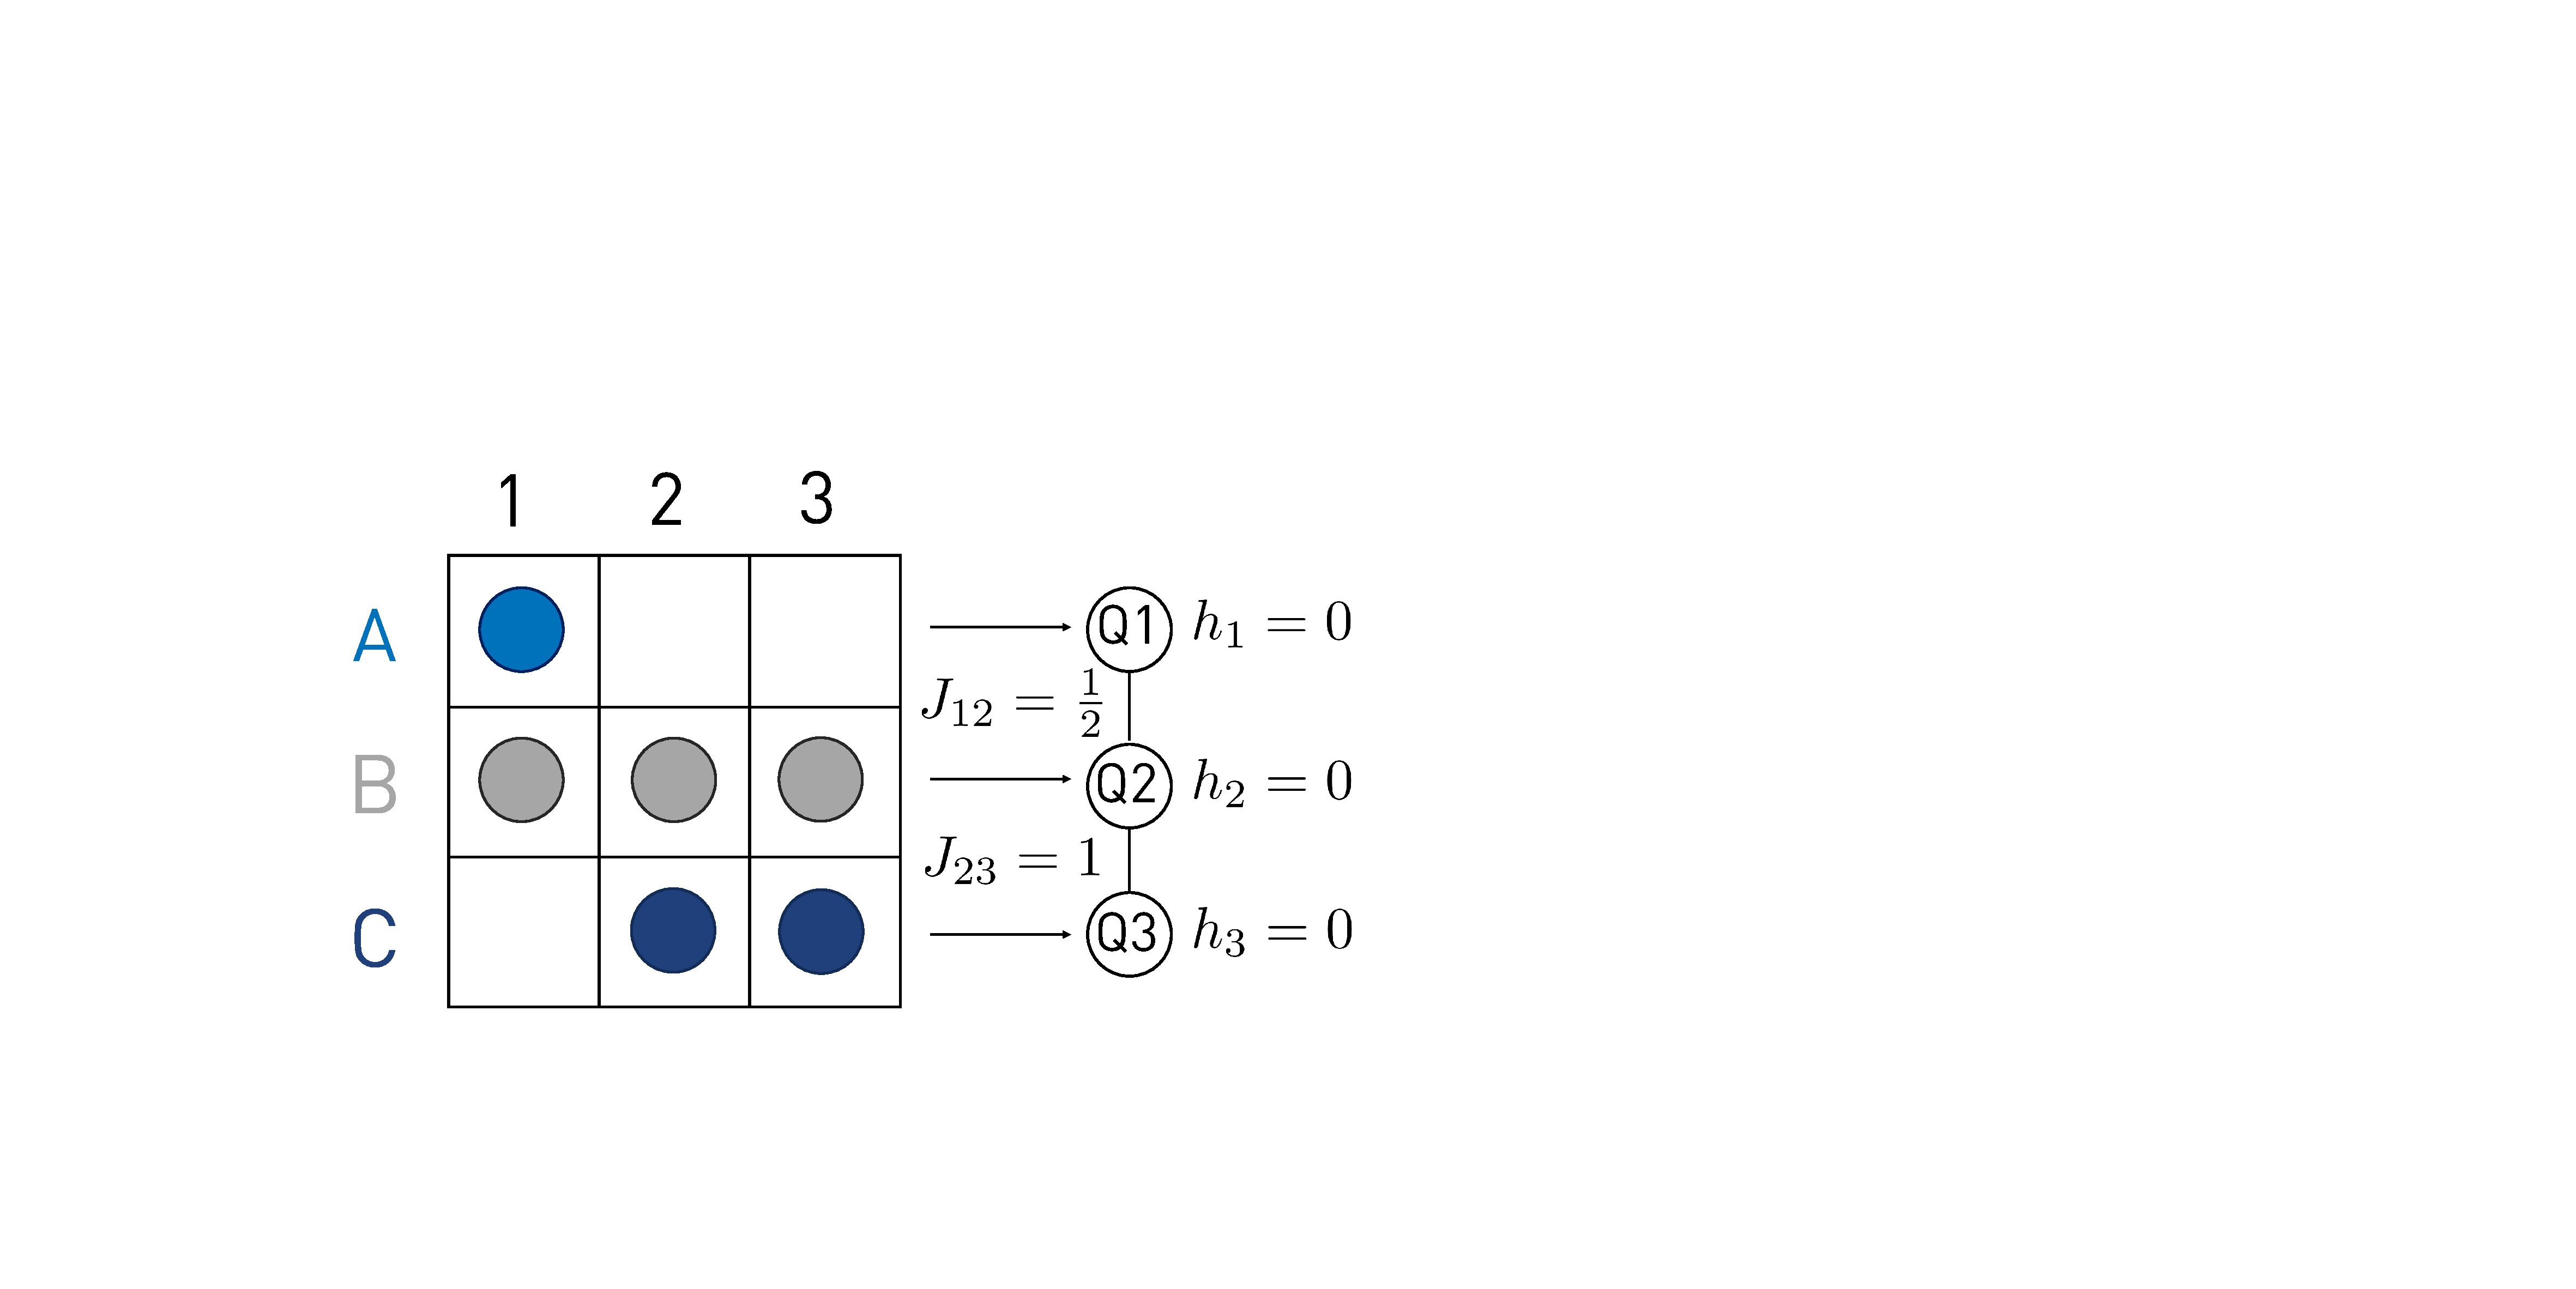
\includegraphics[width=0.8\textwidth, trim={11cm 8cm 38cm 13cm},clip]{chapters/qaoa/figs/exact_cover_matrix.pdf}
    \caption{Incidence matrix representation of the exact cover problem instance implemented in this work. A dot indicates a 1 and an empty square indicates a 0. The mapping to the 3 qubit chain and the corresponding Ising Hamiltonian parameters are indicated on the right hand side.}
    \label{fig:qaoa_exact_cover_matrix}
\end{figure}

\section{Experiment} \label{sec:qaoa_experiment}
In this section, we implement the \gls{qaoa} on a quantum processor to find an approximate solution to a combinatorial optimization problem with 3 qubits. In addition, we compare the performance of the \gls{dir} and \gls{dec} for different depths. We use qubits 1, 2 and 3 of the device presented in Appendix~\ref{app:setup}. Information relative to the single- and two-qubit gates are reported in Appendix~\ref{app:setup}, Table~\ref{tab:cz_gate_params}. All measurements are performed with 3-level single shot readout, see Appendix~\ref{ch:qutrit_readout}. In the context of the \gls{qaoa}, leakage events can be seen as measuring bit strings which do not belong to the space of possible solutions. We therefore condition the measurements outcome on no leakage event. Hence, leakage events reduce the effective number of shots on which we compute estimates. They do not, however, influence the algorithm as long as as the excitation stays in the \f{} level until the state is measured. We make this assumption, as sequences of interest are shorter than $4\,\mu\text{s}$, and the shortest \f{} level $T_1$ is approximately $10\,\mu\text{s}$. All measurements are done without ground state heralding or readout error correction.

\subsection{Cost function landscapes}
Although $p=1$ does not always yield a good approximate solution to the optimization problem, it is a useful intermediate benchmark towards implementing multi-layer \gls{qaoa} circuits ~\cite{Pagano2019QuantumSimulator, Bengtsson2019QuantumProcessor}. A single layer implementation has two variational parameters, $\gamma$ and $\beta$, such that the cost function landscape can be mapped out and visualized with a grid search over $\gamma$ and $\beta$. We make several observations to restrict the search space for each parameter. 

First, if $\hat C$ has only integer eigenvalues\footnote{$\hat C$ is diagonal and therefore elements on its diagonal are the eigenvalues by definition.}, then $\gamma$ is at least $2\pi$-periodic because $\sexp{-\i(\gamma + 2\pi) \hat C} = \sexp{-\i 2\pi \hat C} \sexp{-\i \gamma \hat C} = \sexp{-\i \gamma \hat C}$ since $2\pi \hat C$ yields integer multiples of $2\pi$ for all elements on the diagonal. If in addition the eigenvalues are either all odd or all even, then $\gamma$ shows a periodicity of $\pi$, as $\sexp{i\pi\hat C}$ yields in that case $\pm I$ depending on whether the eigenvalues are all odd or all even. By construction, this is the case when all $J_{nm}$ in $\hat C$ are integers. 

Second, the parameter $\beta$ yields single-qubit $x$-rotations of angle $2\beta$ on all qubits and is therefore at least $\pi$-periodic.

We thus restrict our search space for this problem instance\footnote{In the problem instance we study, the eigenvalues are odd integers multiples of 1/2 and not odd integers. Therefore, the periodicity in $\gamma$ is only $2\pi$ and not $\pi$. We make use of the fact that the landscape is point symmetric around ($\gamma$, $\beta$) = ($\pi$, $\pi/2$) due to the linear connectivity to restrict the search space of $\gamma$ between 0 and $\pi$. Another option would have been to multiply $\hat C$ by a constant factor such that all eigenvalues are integers.} to the domain $(\gamma, \beta) \in [0, \pi] \,\times\, [0, \pi]$. For each parameter pair, we repeat the state preparation and measurement 20000 times to estimate the expectations values $\langle\szsz{1}{2}\rangle$ and $\langle \szsz{2}{3} \rangle$ from which the cost \cost{} is computed.

We execute this measurement with a resolution of 45 points per axis both for the \gls{dir} and the \gls{dec}, and present the result in Fig.~\ref{fig:qaoa_landscapes} along with the landscape obtained with a noise-free unitary evolution (which does not take into account decay and dephasing rates) simulated in QuTip~\cite{Johansson2013QuTiPSystems} .

The simulation reveals two global minima for \cost{} $\approx -1.05$ at $(\gamma, \beta) \approx (\frac{2\pi}{9}, \frac{\pi}{7})$ and $(\frac{2\pi}{9},\pi/2 + \frac{\pi}{7})$.  The landscape also exhibits two pairs of local minima with slightly different depths; one at $\gamma \approx \frac{5\pi}{8}$ and one at $\gamma \approx \frac{7\pi}{8}$ also separated by $\pi/2$ in the $\beta$ direction. The $\pi/2$ periodicity in $\beta$ can be understood intuitively from the Bloch sphere perspective: for $p=1$, we start on the equator and apply parametrized entangling $Z$-rotation between qubits. Each qubit therefore stays on the equator of its Bloch sphere. Thereafter, we apply parametrized $X$-rotations on all qubits which rotate the vectors back towards the $z$-axis\footnote{Except if the vectors are degenerate with the $\pm x$-axis.}. For a $X$-rotation angle larger than $\pi$ (i.e.\ $\beta>\pi/2$), we simply inverse the polarity of all states (all $\ket{1}$ are now mapped to $\ket{0}$ and vice-versa). The correlations between qubits remain unaffected by this polarity inversion and therefore the landscape is periodic.

The locations of all extrema in the measurements are in good agreement with the simulations, suggesting a low amount of total coherent errors. Incoherent errors due to decoherence affect the contrast of the landscapes, resulting in a minimum measured cost of $\sim -0.95$ ($\sim -0.85$) for the direct (decomposed) implementation. The decomposed implementation does not reach the same cost value as its gate sequence is longer and thereby more affected by decoherence. In addition, it suffers more from coherent errors than the direct implementation. The latter are caused predominantly by residual $ZZ$-coupling, and therefore accumulate over the longer sequence. The combination of these effects could explain the diagonal feature observed in its landscape, which does not appear as strongly for the direct implementation. The average total leakage (any qubit measured in the \f-level) amounts to 4.5\% for the direct implementation and 7.8\% for the decomposed implementation. Most of the leakage occurs due to the two-qubit gate between qubit 1 and qubit 2, which suffers from higher leakage (see Appendix~\ref{app:setup}, Table~ \ref{tab:cz_gate_params} for a detailed discussion).

Note that even in the noise-free simulation, \cost{} never reaches its minimum value of -1.5 thereby indicating that the performance of the algorithm is limited by the chosen depth of $p=1$. Nevertheless, additional layers introduce new variational parameters, making grid search quickly intractable. Therefore, we use a classical optimizer to find the optimal variational parameters.

\begin{figure}[ht]
    \centering
    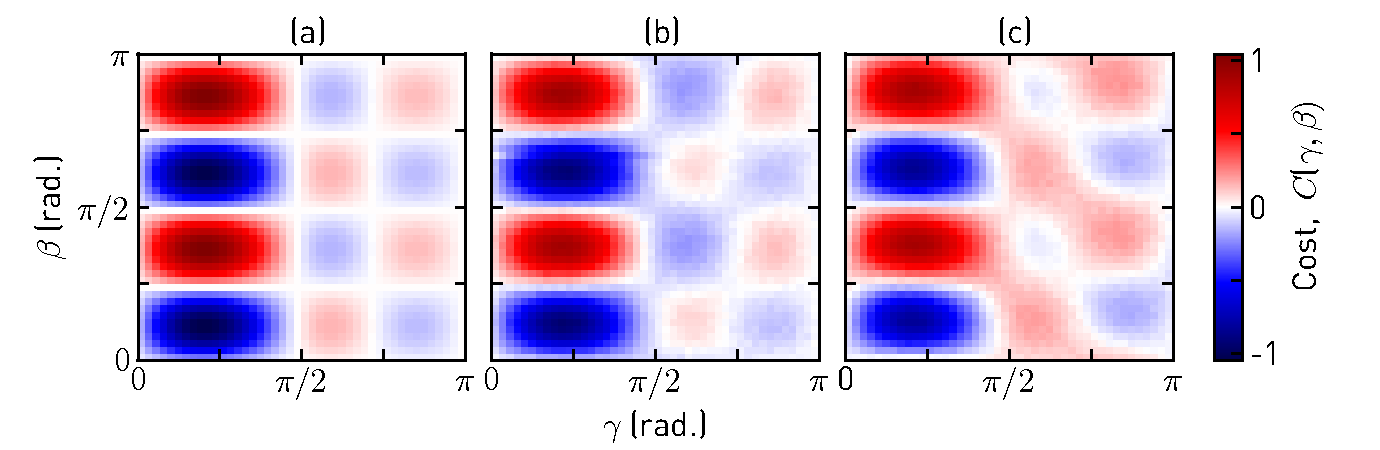
\includegraphics[width=\textwidth]{chapters/qaoa/figs/qaoa_landscapes_20200216_211657.pdf}
    \caption{Optimization landscapes for a \gls{qaoa} implementation with one layer. The two variational parameters, $\gamma$ and $\beta$ are swept over a 45x45 grid, and the cost function $\cost$ is evaluated for each parameter pair.  (a) Landscape obtained with noise-free simulation. The minimal cost function value is approximately -1.05. (b) Landscape obtained with the direct implementation of the \gls{carb}. Taken with 20000 single shot measurements per parameter pair. (c) Landscape obtained with the decomposed implementation of the \gls{carb}. Taken with 20000 single shot measurements per parameter pair. }
    \label{fig:qaoa_landscapes}
\end{figure}


\subsection{Variational parameter optimization} \label{sec:qaoa_optimization}
When no strategy is known to find the best variational angles and  $p > 1$,  classical optimizers constitute a way to navigate through the parameter space. Desirable properties to ensure rapid and consistent convergence to the optimal parameters are:
\begin{itemize}
    \item [--] \textbf{Low cost function sampling}. Each query to the quantum computer is costly in time. Therefore, optimizers minimizing the number of queries sent to the quantum computer are better suited for this task. Algorithms relying on Hessian matrix estimation are not suited, as the number of elements in the Hessian matrix grows quadratically with $p$.
    \item[--] \textbf{Robustness to noise}. Measurements from quantum computers are subject to noise. Especially when the gradient of the cost function is small, it is crucial for the algorithm to be robust to fluctuations.
    \item[--] \textbf{Capability of avoiding local minima}. At low depths, the cost functions show local minima. Algorithms capable of finding the global optimum are better suited.
\end{itemize}

We leave the task of finding the optimal classical optimizer for future work, and instead focus on comparing the performance difference of a simple optimizer between the \gls{dir} and \gls{dec}
For the sake of completeness, we briefly report on optimizers which have been applied to \gls{qaoa} in recent literature.

To find variational parameters for a single layer \gls{qaoa} implementation, Ref.~\cite{Otterbach2017UnsupervisedComputer} applied Bayesian optimization (BO)~\cite{Mockus1989GlobalApproach}, a gradient-free, global optimization method relying on Gaussian processes. Although BO performs excellently in low-dimensional parameter spaces, the number of evaluations grows exponentially with the number of parameters, rendering it impractical when $p$ is large. Ref.~\cite{Bengtsson2019QuantumProcessor} compared BO on a two-layer \gls{qaoa} implementation with the Nelder-Mead (NM) algorithm~\cite{Nelder1965AMinimization} and the covariance matrix adaptation evolution strategy (CMA-ES)~\cite{Hansen2016TheTutorial}. On their problem instance, NM has the lowest cost function sampling but is also the most sensitive to local minima due to its locality. By contrast, the CMA-ES requires more function evaluations but is stochastic and is believed to scale favorably with the number of parameters~\cite{Bengtsson2019QuantumProcessor}. For $p=2$, BO yielded a good trade-off between low cost function sampling and sensitivity to local minima. 
Ref.~\cite{Pagano2019QuantumSimulator} used problem-specific heuristics combined with a bootstrapping algorithm. Other heuristics~\cite{ZhouQuantumDevices} and deep-learning based approaches~\cite{Verdon2019LearningNetworks} have been proposed but not tested beyond simulations. Finally, the simultaneous perturbation stochastic approximation (SPSA)~\cite{Bhatnagar2013StochasticOptimization} is a promising stochastic global optimization approach not yet applied to \gls{qaoa}. The major advantage of SPSA is that it requires only two cost function evaluations per optimization step, independently of the dimensions of the parameter space.

In this work, we use the NM algorithm, due to its simplicity and low cost function sampling. To mitigate the effect of local minima, we increase the size of the initial simplex to the same order of magnitude as the distance between minima observed in Fig.~\ref{fig:qaoa_landscapes}.

 For each optimization trajectory, we initialize parameters randomly and then let the NM algorithm run 40 cost function evaluations. One function evaluation takes approximately 20-25 seconds such that an optimization trajectory takes approximately 12 minutes. In Fig.~\ref{fig:qaoa_optimization_traces}, we show the results of 15 optimization trajectories of both implementations for up to 4 \gls{qaoa} layers. Each data point of the cost function is estimated from 20000 shots. 

\begin{figure}[ht]
    \centering
    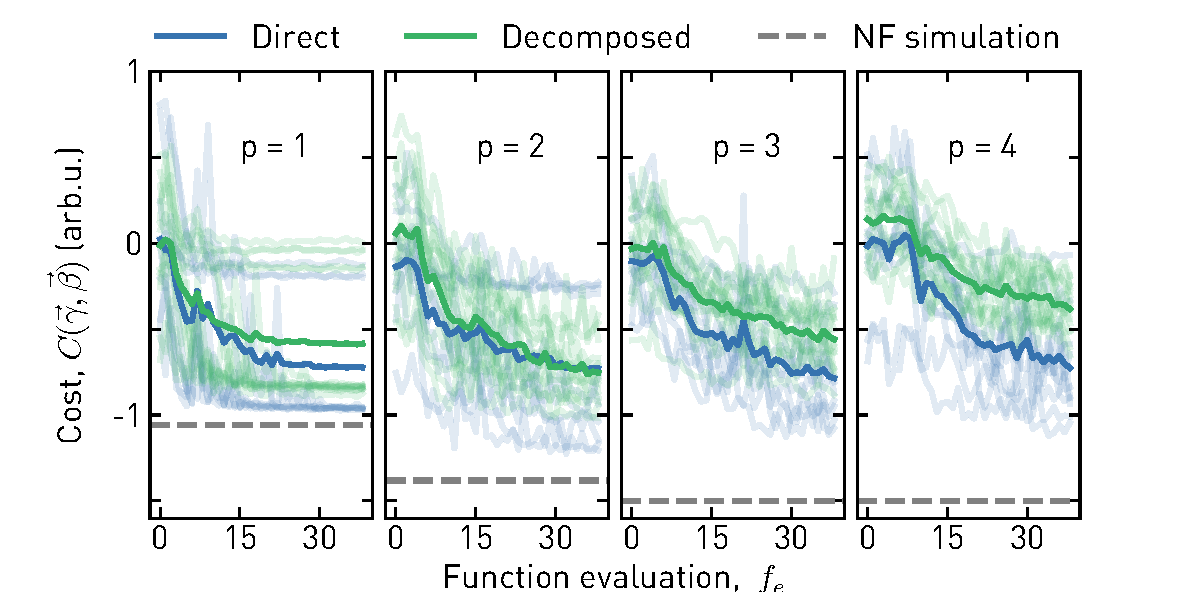
\includegraphics[width=\textwidth]{chapters/qaoa/figs/ch5_qaoa_optimization_traces_one_line_20200205_212444.pdf}
    \caption{Cost optimization trajectories for depths of $p=$ 1, 2, 3 and 4 as a function of the number of function evaluations, $f$. The variational parameters are initialized randomly and then optimized iteratively with the Nelder-Mead algorithm. Each cost value is computed from 20000 single shot measurements. The trajectories obtained with the direct (decomposed) implementation of the \gls{carb} are shown in blue (green). The faded lines correspond to the 15 individual trajectories while the darker color correspond to their average. The grey dashed line indicates the minimal achievable cost for each depth as calculated with a noise-free simulation.}
    \label{fig:qaoa_optimization_traces}
\end{figure}

The motivation for a higher number of layers becomes apparent. For $p=1$, we observe for either implementation three different convergence values of the cost function, two corresponding to the local minima and one to the global minimum, as expected from the three pairs of minima visible in Fig.~\ref{fig:qaoa_landscapes}. The local minima significantly impact the average cost at convergence. In addition, the best case performance is limited by the minimal achievable cost for $p=1$.

For $p=2$, the best trajectories of the direct implementation achieve cost below what is possible with only one layer and local minima are less apparent, although still present. 

 Three layers are required to reach the minimum cost of $-1.5$ in noise-free simulation. But adding layers does not always yield better performance. Indeed, it also results in longer gate sequences, aggravating the effect of decoherence. Moreover, additional layers increase the dimension of the parameter space, resulting in slower convergence, which is clearly visible by comparing the average trajectories for e.g.\ 1 and 4 layers. In fact, the average trajectories suggest 40 cost function evaluations do not allow the algorithm to fully converge for $p > 1$. 

For $p = 1,3,4$, the direct implementation reaches lower cost on average (for $p=2$, only its median is lower), indicating that the gate sequence length plays a major role in the performance of the algorithm. In the next section, we analyze this effect in more details. 

\subsection{Success probability as function of depth}
The previous section suggests there is an inherent trade-off: additional layers increase the performance of the algorithm in theory but also aggravate the effect of sequence-length-dependent errors in experiments. Similar conclusions were found by Alam et al.~\cite{Alam2019AnalysisQubits}. The goal of this section is to analyze how this trade-off affects the two implementations of the \gls{qaoa}.

Note that the (approximate) solution of a problem found with \gls{qaoa} is the measured bit-string after optimization of the variational parameters. Therefore, a crucial metric to assess the performance is the success probability, $P_s$ (see Section~\ref{sec:qaoa_success_prob}) and not the cost function used for classical optimization of the variational parameters. 

To investigate the effect of the depth $p$ on $P_s$ accurately, we seek to mitigate the influence of the classical optimizer on $P_s$ (namely, the influence of local minima and the convergence speed, which are expected to be equal for both implementations). To this extend, we provide an educated initial guess for the variational parameters. Namely, we first find optimal parameters for each depth in a noise-free simulation and provide these theoretically optimal parameters for the initialization of the quantum computer. Under the assumption of equal depolarization, bit-flip and dephasing channels for all qubits, the optimal variational parameters remain nearly the same in a noise-free and noisy environment, according to a recent theoretical investigation~\cite{Xue2019EffectsAlgorithm}. Because coherence times and coherent errors are not exactly equal for all qubits on our device, we additionally optimize locally with up to 20 function evaluations on the quantum computer. 

We show the result of the above-mentioned protocol in Fig.~\ref{fig:qaoa_sequence_lengths}. The success probability for various depths is plotted versus sequence length, $L$, to facilitate the comparison of sequences of similar lengths independently of the implementation. The dashed lines correspond to the expected success probability in a noise-free environment. 

\begin{figure}[ht]
    \centering
    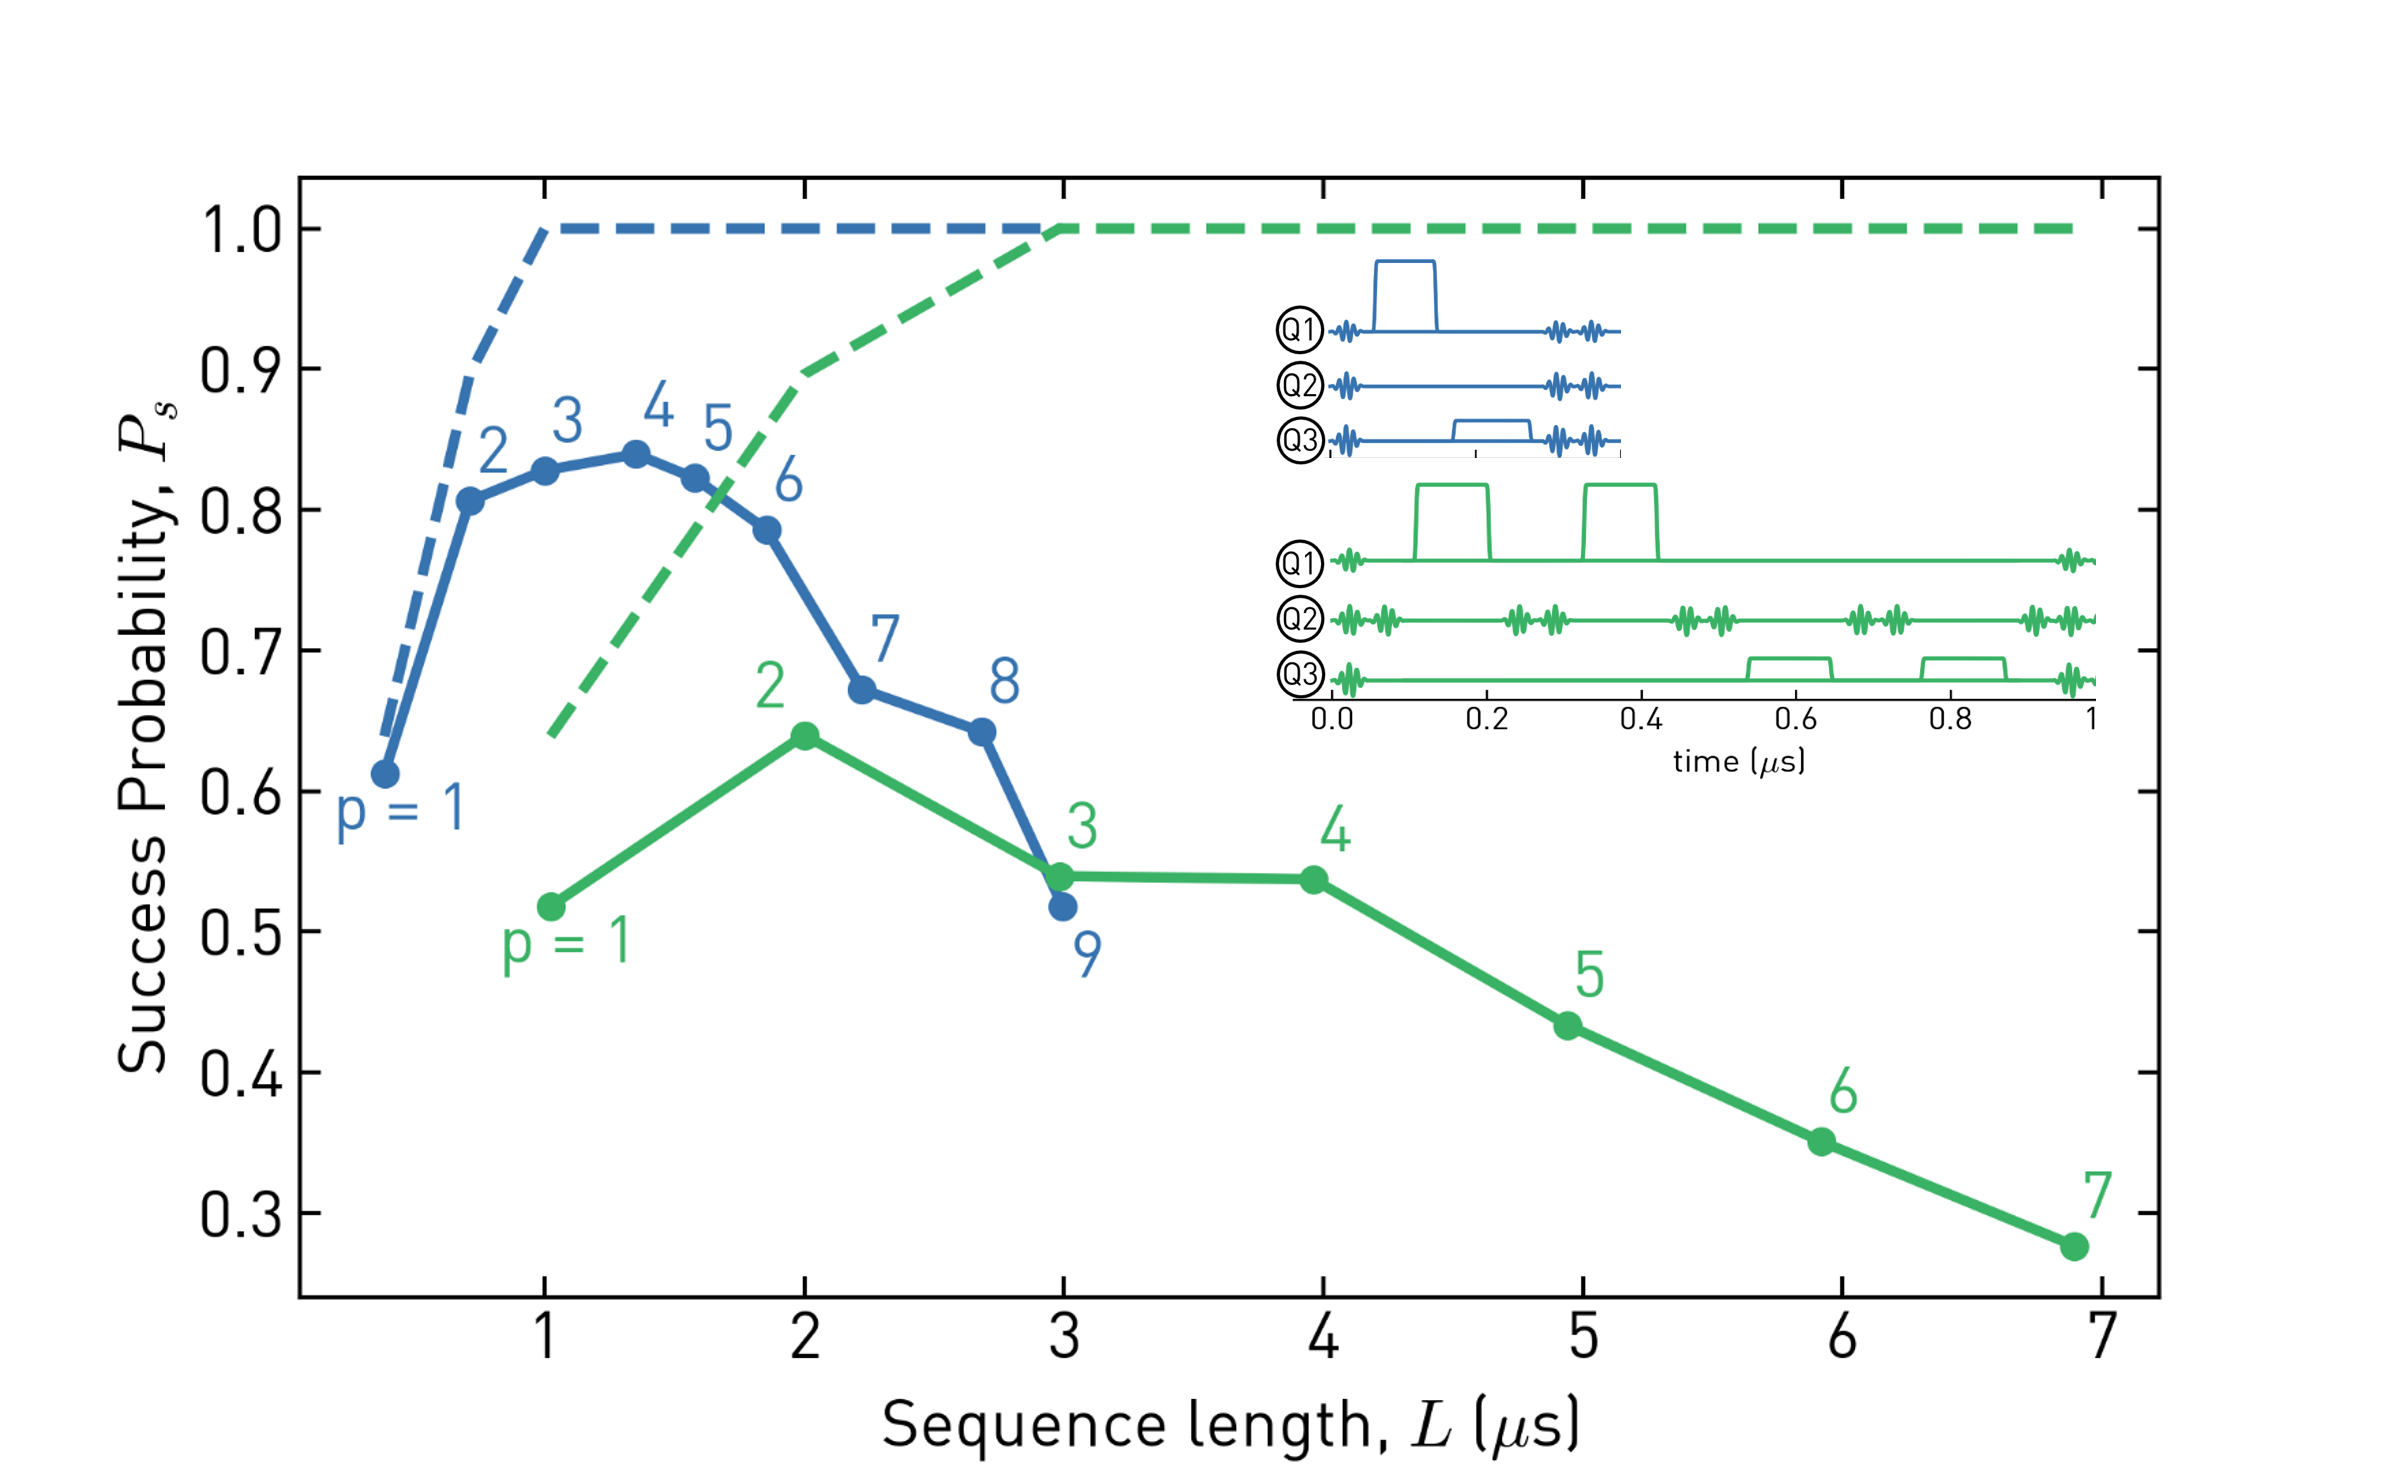
\includegraphics[width=\textwidth]{chapters/qaoa/figs/ch5_qaoa_sequence_lengths_v1_withinset_20200202_120000.png}
    \caption{Success probability as a function of sequence length for the direct (blue) and decomposed (green) implementations of the \gls{carb}. The dashed line of corresponding color indicates the success probability as calculated by a noise-free simulation. The depth is annotated next to the data points. For each depth, the quantum computer is initialized with variational parameters obtained from the noise-free simulation. The corresponding pulse schemes for one layer are shown in the inset.}
    \label{fig:qaoa_sequence_lengths}
\end{figure}

The \gls{dir} exhibits a clear advantage: in about $1\,\mu\text{s}$, it is able to execute a 3 layers of \gls{qaoa} while the decomposed implementation only carries out one. For a fixed depth, it consequently suffers less from errors scaling with the sequence length. 

The difference in sequence length arises from the combination of two factors (see inset of Fig.~\ref{fig:qaoa_sequence_lengths} for the full pulse sequence for $p=1$):
\begin{enumerate}
    \item The decomposition of each \gls{carb} requires two individual \gls{cz} and 4 single-qubit gates. 
    \item The \gls{carb} is shorter than the \gls{cz} for any conditional phase different from $\pi$.
\end{enumerate}
Moreover, the number of \glspl{carb} grows with $\mathcal{O}(m\cdot p)$, where $m$ indicates the number of two-qubit terms in \costh{} which cannot be executed simultaneously. Therefore, the total decomposed sequence length rapidly becomes much longer. 

As mentioned in Section~\ref{sec:qaoa_optimization}, noise-free simulations require in the ideal case 3 layers to reach $P_s \approx 1$, which for the \gls{dec} is realized with $L \approx 3\, \mu\text{s}$. For that sequence length, the \gls{dir} can implement up to nine layers. However, in Fig.~\ref{fig:qaoa_sequence_lengths} we observe that both implementations show similar performance for $L \approx 3\, \mu\text{s}$, which directly indicates that performance is limited by sequence length rather than the number of layers.
In particular, in our case we expect both conditional phase errors due to residual $ZZ$-coupling and decoherence to have a major impact which scales with sequence length.

To gain further insights into the performance of the algorithm, we present in Fig.~\ref{fig:qaoa_state_histogram} the full distribution of measured bit strings for each of the first 4 points ($p=1,2,3,4$ for each implementation) of Fig.~\ref{fig:qaoa_sequence_lengths}. The colored dots in the right panel indicate the respective success probabilities, i.e.\ the sum of the probabilities for states $\ket{010}$ and $\ket{101}$ (colored bars). The right panel also shows the success probability distribution (faded filling) of the optimization trajectories discussed in Section~\ref{sec:qaoa_optimization}. If the trajectories constitute a representative sampling of the parameter space, the dot should lie at the right edge of the distribution. A data point outside the distribution suggests the trajectories did not converge to the lowest possible value, or did not find the global cost optimum, for instance because of a local minimum. Conversely, a data point inside the distribution suggests the initialization from theoretically optimal variational parameters is not perfect, or fluctuating performance compared to when the trajectories were recorded.

\begin{figure}[ht]
    \centering
    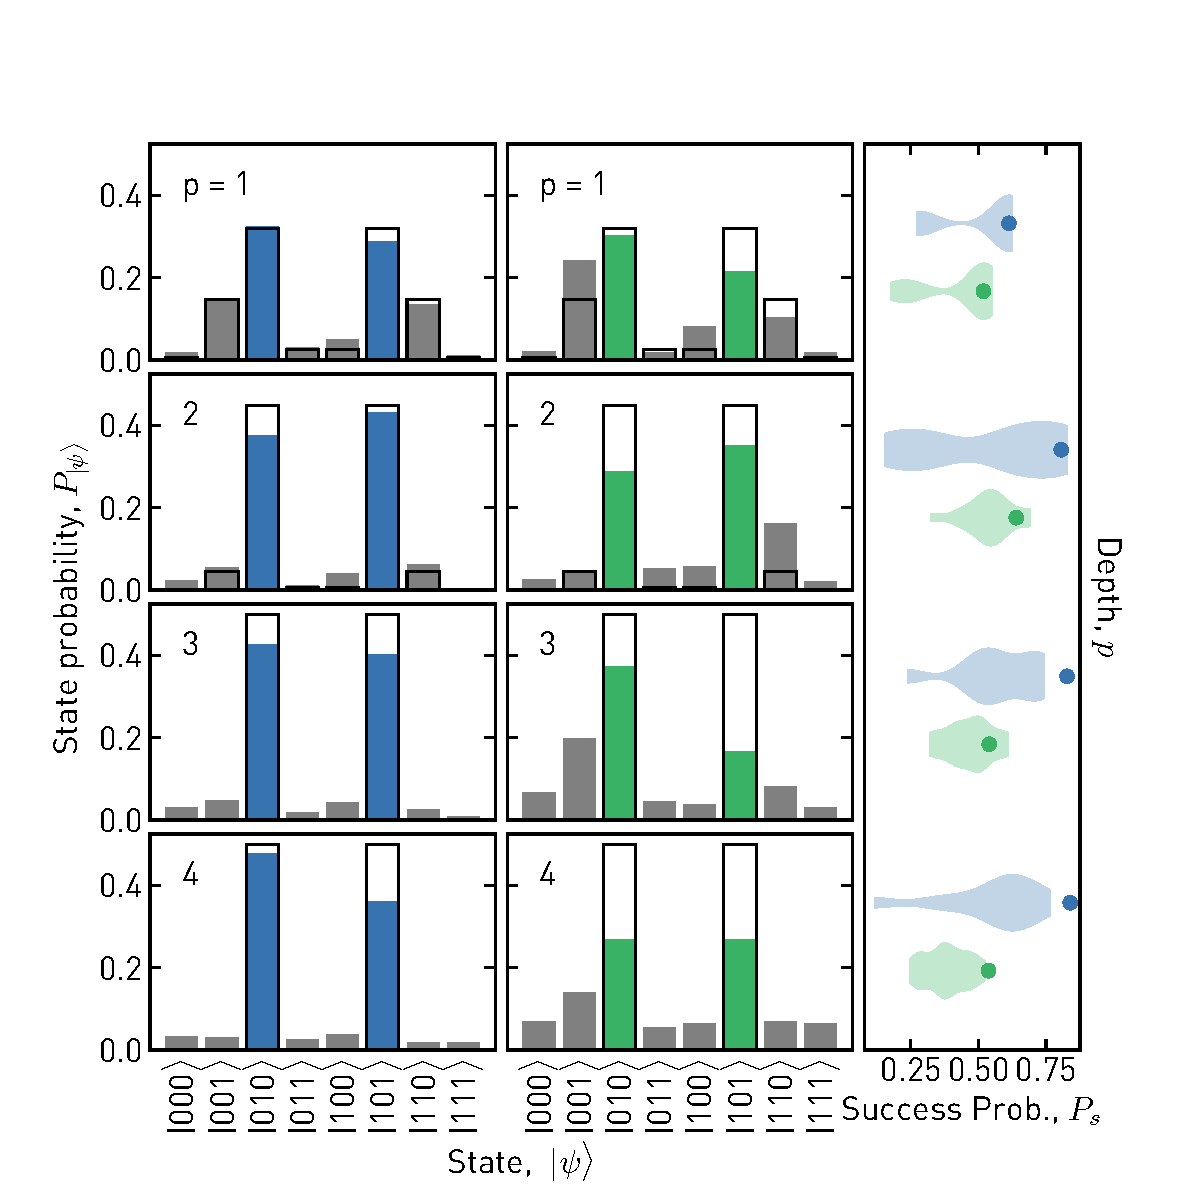
\includegraphics[width=\textwidth]{chapters/qaoa/figs/ch5_qaoa_state_histograms_20200202_134816.pdf}
    \caption{Distribution of measured states for the \gls{dir} (left) and \gls{dec} (middle) for $p=1,2,3,4$. The black wire-frame corresponds to the noise-free simulation distribution of states and is equal for both implementations, at fixed depth. For each distribution, the highlighted bars correspond to solutions of the exact cover problem. Their sum amounts to $P_s$, shown on the right panel with dots of corresponding color (also corresponding to the first 4 dots for each implementation in Fig.~\ref{fig:qaoa_sequence_lengths}). The faded distributions in the right panel correspond to the success probability of the optimization trajectories presented in Fig.~\ref{fig:qaoa_optimization_traces}.}
    \label{fig:qaoa_state_histogram}
\end{figure}

In the state distributions, the most likely states are $\ket{101}$ and $\ket{010}$, corresponding to the desired sets $\mathcal{L}_1' = \{A,C\}$ and $\mathcal{L}_2' = \{B\}$ defined in Section~\ref{sec:qaoa_exact_cover}. The \gls{dir} is in excellent agreement with the noise-free simulation (black wire-frame) for all depths, and achieves a success probability of $0.84$ at $p=4$\footnote{In principle three layers are sufficient to reach $P_s \approx 1$ and additional layers are expected to suffer from additional errors, thereby showing a decrease in success probability. However, the classical optimizer also allows to compensate for some errors and more parameters provide additional degree of freedom to correct for errors.}. By contrast, the \gls{dec} consistently shows more deviations from the simulation and achieves a maximal success probability of $0.64$\footnote{Note that one of the optimization trajectory starting from random initialization reaches a success probability of $0.69$ at $p=2$. We attribute this difference to fluctuations in coherence times and gate performance} at $p=2$. 

We conclude that the trade-off of additional layers affects the two implementations of the \gls{carb} differently. The success probability of the \gls{dir} increases for up to four layers before being decreasing due to decoherence and accumulated phase errors, thereby achieving a success probability of 0.84. On the other hand, the \gls{dec} can only execute two layers before being affected by sequence length dependent errors, which is not sufficient to reach the regime where the success probability is near unity even in the noise-free simulation.

\section{Conclusion}
\glsreset{qaoa}

In this chapter, we have found approximate solutions for a three-qubit exact cover problem instance using the \gls{qaoa}. The problem instance requires at least three layers of the \gls{qaoa} in the ideal case to reach a success probability approaching unity, as determined by noise-free simulations. To the best of our knowledge, this constitutes the deepest problem considered in the experimental \gls{qaoa} literature. 

We have shown that for this problem instance, the direct implementation of two-qubit interaction terms in each layer of the \gls{qaoa} reduces the two-qubit gate-count by 50\% and the executed gate-sequence length by a factor of $\sim 3$ compared to a decomposition into 2 \glspl{cz} and 4 single-qubit gates. Exploiting this advantage, we demonstrate a success probability of $0.84$ using 4 layers of \gls{qaoa}. In comparison, the decomposed implementation reached a maximal success probability of $0.64$ with 2 layers as it is more affected by decoherence and residual $ZZ$-coupling. Experimental observations also strongly suggest that decoherence and residual $ZZ$-coupling are the dominant error sources in both implementations.

The sequence length reduction factor enabled by \glspl{carb} scales approximately linearly with the number of two-qubit terms in the cost Hamiltonian which cannot be executed simultaneously. Typically, the number of two-qubit terms grows with the number of qubits in the problem instance. We therefore expect a considerable performance gain on near-term quantum processors with 10-1000 qubits, as a linear reduction in sequence length avoids exponentially increasing incoherent errors.  In summary, this work provides tangible evidence that \glspl{carb} open the door to solving more complex problem instances on quantum computers for as long as the algorithm's performance are limited by decoherence. 


\chapter{Conclusion}
\glsresetall{}

% Large-scale, fault-tolerant quantum computing has the potential to impact numerous fields such as chemistry, medical research, material science, information security and logistics. However, building large-scale and noise-free quantum computers is a substantial challenge. Consequently, near-term quantum computers will only have a limited number of quantum bits (qubits) and a limited computing time during which operations are executed reliably.

% \Glspl{vqa} are good candidates to take advantage of the quantum hardware in the near-term because they offset part of the computation to classical computers and are intrinsically more robust to noise mostly because they seek approximate solutions. The available computation time remains nevertheless limited by time-dependent errors such as decoherence and residual $ZZ$-coupling.

In  this  thesis,  we  demonstrated  a  way  to  enhance  the  performance  of \glspl{vqa} by reducing the  sequence length  required  to implement their circuit on quantum hardware. In particular, we enlarged the gate-set available on the quantum computer with a \gls{carb}, which enables us to avoid decomposition of higher order operations into multiple gates. 

The \gls{carb} is a generalized version of the controlled $\pi$-phase two-qubit gate (CZ gate). It is able to reach any phase on the \oo{} state between 0 and $2\pi$. Our implementation achieves an average process fidelity of 97.7\%, whereby the remaining errors are dominated by decoherence and effects of thermal population. The average leakage per gate amounts to 1.4\%, which is slightly lower than the leakage we obtain for a CZ gate implemented on the same physical qubits.

We demonstrated the advantage of \gls{carb} on a three qubit exact cover problem instance which we solved using the \gls{qaoa}, a \gls{vqa} that finds approximate solutions to combinatorial problems.  The instance we considered is the first experimental implementation requiring three QAOA layers to be solved with high success probability. 

We obtain a 50\% two-qubit gate count reduction and a gate sequence length reduction factor of 3 using the direct implementation of the \gls{carb} compared to a decomposition into \glspl{cz} and single qubit gates. Consequently, we achieve a higher success probability with the direct implementation (0.84 versus 0.64) because it executes more layers for a fixed sequence length. 

We foresee an even more pronounced advantage for larger-scale experiments because the number of layers required to solve problems typically scales with the number of qubits involved in the experiment. Therefore, for as long as quantum devices are limited by decoherence, \glspl{carb} will open the door to solving more complex problem instances with \gls{vqa}.

\chapter{Outlook} \label{ch:outlook}
While \glspl{carb} will provide a considerable performance advantage for larger quantum computers in the NISQ era, their up-scaling to larger systems also entail new challenges and open questions.

A first challenge relates to the elaborate \gls{carb} calibration procedure, although a few straight-forward improvements are expected to increase the calibration speed by an order of magnitude (see Section~\ref{sec:carb_calibration}). While we implemented the gate for fixed-coupling,  frequency-tunable transmons using unipolar flux pulses, other gate architectures might provide a higher level of convenience. One promising approach is a gate based on a tunable $ZZ$-coupling achieved with a frequency tunable coupler qubit \cite{Collodo2020}.  Independently of the flux pulse parametrization, this gate acquires conditional phase linearly as function of interaction time which eases the calibration and potentially reduces interpolation errors. In addition, the acquired dynamic phase changes slowly as a function of other gate parameters, which reduces the number of calibration points and therefore the overall tune-up time of the gate. 

Developing rapid and adequate characterization techniques for continuously parametrized gates designed for \glspl{vqa} is a second aspect arising from this thesis, and is not clearly established in literature. Although quantum process tomography provides full information about the quantum process, it also suffers from leakage, preparation errors and does not offer an intuitive interpretation for the different error sources. 

Inspired from Ref.~\cite{Abrams2019ImplementationPulse}, we propose an alternative characterization method for benchmark pairs of subsequent gates, with conditional phases of $\pi-\alpha$ and $\alpha$ respectively. Since the conditional phase of these two gates sums up to $\pi$, the combination of the two gates corresponds to a \gls{cz} which is in the Clifford group.  Randomized benchmarking therefore allows to put a bound on the error of the combination of two gates (but not on the individual gates). Cross-entropy benchmarking \cite{BarendsDiabaticQubits} is another approach that can assess the performance of non-Clifford gates and has been used by Ref.~\cite{Foxen2020DemonstratingAlgorithms} for their continuously parametrized gates.

However, both randomized and cross-entropy benchmarking are insensitive to small coherent errors which can accumulate quickly and cause deleterious effects in algorithms with repetitive structures (such as \gls{qaoa}) \cite{Kjaergaard2020AProcessor}. A recent calibration method based on quantum process tomography of long strings of CZ gates alleviate these effects \cite{Kjaergaard2020AProcessor} and could be extended to \glspl{carb}.

As we progress towards larger experiments, we will have the opportunity to explore more complex problem instances. In Fig.~\ref{fig:outlook_problem_instances}(b) and (c), we present two exact cover problem instances designed for the device described in Ref.~\cite{Andersen2019RepeatedCode}, whose hardware connectivity graph is reproduced in Fig.~\ref{fig:outlook_problem_instances}(a). The former instance respects the connectivity of the device and has two solutions, $\mathcal{L}_1 = \{A, D, G\}$ and  $\mathcal{L}_2 = \{B, C, E, F\}$. By contrast, the latter instance represents a dense problem graph that require interactions between qubits which are not physically connected and has a single answer, $\mathcal{L} = \{C, E, F\}$. The implementation thereof requires SWAP-gates which lengthen the gate sequence for each \gls{qaoa} layer. While the SWAP-gates themselves can be decomposed into \glspl{cz} and single qubit gates, the sequence would be much shorter if the SWAP operations are part of the available hardware gate set. Due to the higher problem graph connectivity and the uniqueness of the solution, the number of layers required to find a good approximate solution is higher for the second problem instance. 

\begin{figure}[ht]
    \centering
    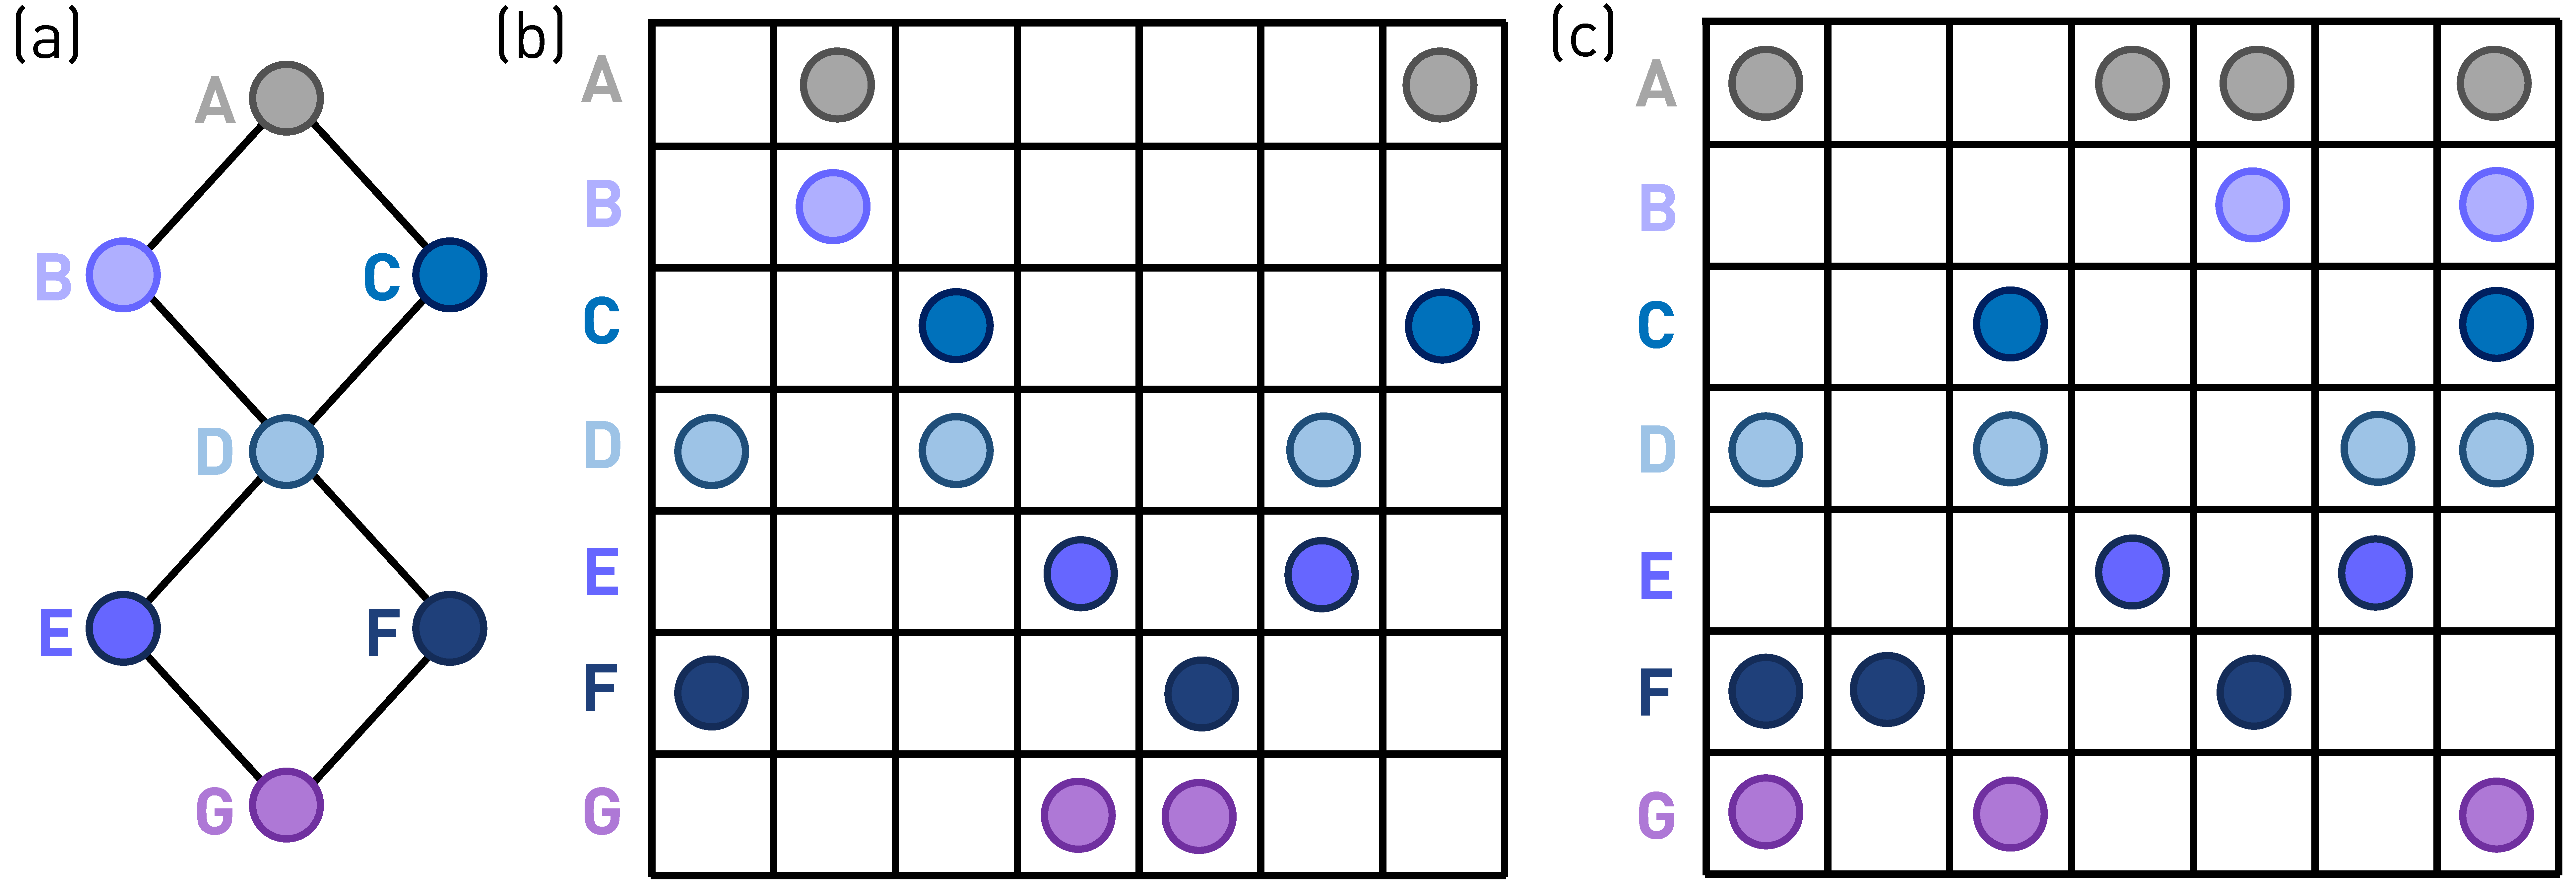
\includegraphics[width=\textwidth]{outlook_problem_s7.pdf}
    \caption{Example of future experiments designed for a 7-qubit quantum processor. (a) Hardware graph connectivity of the 7-qubit quantum processor described in Ref.~\cite{Andersen2019RepeatedCode}. (b) Incidence matrix of an exact cover problem instance respecting the connectivity of (a). (c) Incidence matrix of an exact cover problem instance requiring full "logical" connectivity and therefore SWAP operations between the physical qubits. }
    \label{fig:outlook_problem_instances}
\end{figure}

Finally, the use of the \gls{carb} is foreseen to extend beyond \gls{qaoa}, with potential applications in quantum chemistry~\cite{Jiang2018QuantumFermions} and quantum neural networks~\cite{Cao2017QuantumComputers}.

\appendix

\chapter{Setup}
\label{app:setup}
In this Appendix, we provide additional information with respect to the quantum processor and the experimental setup used for this thesis. In Fig.~\ref{fig:BF1_device_picture}, we present an optical micrograph of the four-qubit quantum processor, from which we use the first three in this thesis.

\begin{figure}[htp]
  \centering
 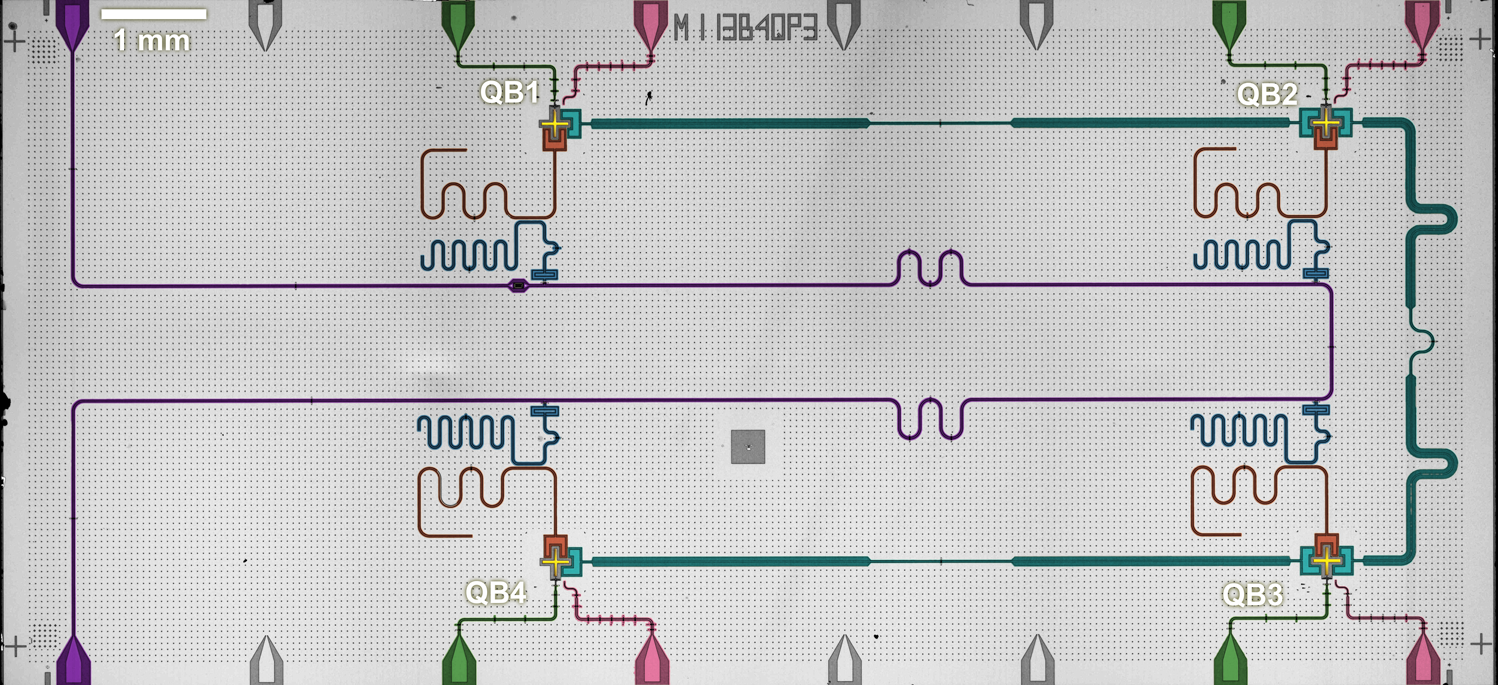
\includegraphics[width=\textwidth]{appendices/setup/figs/BF1_device.png}
 \caption{False-colored optical micrograph of the four-qubit quantum processor. The transmon qubits are colored in yellow, coupling resonators in
cyan, flux lines for single-qubit tuning in green, charge lines for single-qubit manipulation in pink, a common feedline for readout in purple,
and transmission line resonators for readout and for Purcell filtering in red and blue, respectively. Figure and caption text adapted and reproduced from Ref.~\cite{Andersen2019a}.}
 \label{fig:BF1_device_picture}
\end{figure}

In Fig.~\ref{fig:experimental_setup}, we show the detailed schematics of the the experimental setup with all relevant instruments. We use a \gls{uhf} for readout pulse generation and data acquisition, a \gls{hdawg} for single qubit pulse generation, the flux \gls{awg} for two-qubit gate flux pulses generation and a trigger \gls{awg} to synchronize all instruments. The readout line consists of a traveling-wave parametric amplifier (TWPA), a high-electron-mobility transistor (HEMT) amplifier, and the warm amplifier board (WAMP). The filters and attenuators are indicated at each temperature stage of the cryogenic system.

\begin{figure}[htp]
  \centering
 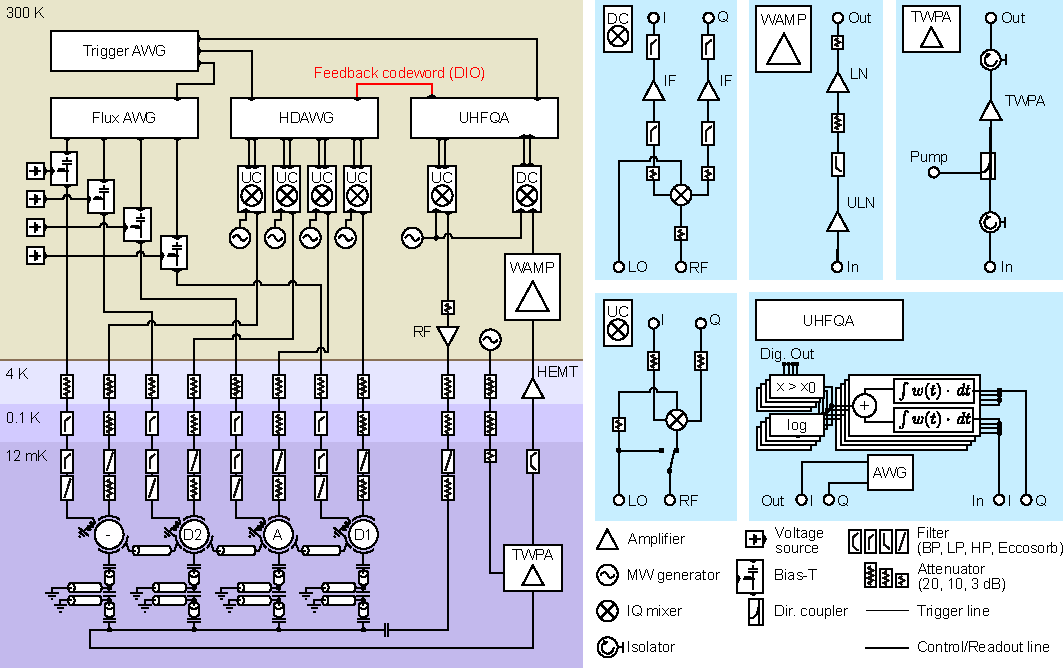
\includegraphics[width=\textwidth]{appendices/setup/figs/setup.pdf}
 \caption{Detailed schematics of the experimental setup. The filtering of the input and output signals including low-pass (LP), band-pass (BP) and infrared-blocking Eccosorb filters and attenuators are shown at the indicated temperature stages.
Extended schematics of the components of the readout chain are shown in the light blue panels. The readout signal is amplified using a traveling-wave parametric amplifier (TWPA), a high-electron-mobility transistor (HEMT) amplifier, and the warm amplifier board (WAMP) consisting of an ultra-low-noise (ULN) amplifier, a low-noise (LN) amplifier and a high-pass (HP) filter. The \gls{uhf} supports weighted integration, data logging (log) and thresholding ($x > x0$) of the readout signal. Figure and caption text reproduced and adapted from Ref.~\cite{Andersen2019}}
 \label{fig:experimental_setup}
\end{figure}

In Table~\ref{tab:app_setup_qubit_params}, we report the qubit parameters including coherence times, thermal populations and 3-level readout correct assignment probability extracted as detailed in Appendix~\ref{ch:qutrit_readout}.

\begin{table}[ht]
\centering
\caption{Coherence, frequency, coupling, and readout properties of the three qubit used in this thesis. The $T_1$ and $T_2$ times are measured at the maximum qubit frequency for qubit 1, and at the minimum qubit frequency for qubits 3. Qubit 2 is not tunable. RO stands for readout. Parameters followed by an asterisk (*) are reproduced from Ref.\  \cite{Andersen2019a}. See Ref.\ \cite{Andersen2019} for multiplexed readout.} % coherence times taken from timestamp 20191129_135651
\label{tab:app_setup_qubit_params}
\begin{tabularx}{\textwidth}{llll}
\toprule
Parameter & \textbf{Q1} & \textbf{Q2} & \textbf{Q3} \\ 
\midrule
Maximum qubit frequency* (GHz) & \multicolumn{1}{c}{5.721} & \multicolumn{1}{c}{5.210} & \multicolumn{1}{c}{5.530} \\
Minimum qubit frequency* (GHz) & 5.083 & 4.880 & 4.386  \\
Qubit lifetime ($\mu$s) & 27.8 & 16.3 & 22.9  \\
Qubit Ramsey coherence time ($\mu$s) & 25.4 & 20.0 & 12.5  \\
Qubit echo coherence time ($\mu$s) & 32.4 & 22.8 & 22.4 \\
Readout resonator frequency (GHz) & 6.890 & 7.085 & 6.686  \\
Purcell resonator – RO resonator detuning* (MHz) & 29.5 & 27.5 & 19.4 \\
Purcell resonator – RO resonator coupling* (MHz) & 10.9 & 8.2 & 9.5 \\
Purcell resonator to half-feedline coupling* (MHz) & 27.2 & 34.7 & 10.7 \\
Effective readout resonator linewidth* (MHz) & 2.4 & 2.0 & 1.5  \\
Dispersive shift* (MHz) & -3.9 & -1.6 & -1.8 \\
Thermal population (\%) & 0.9 & 0.4 & 1.4  \\ 
3-level RO assignment prob. (no preselection) (\%) & 97.42 & 96.57 & 95.71\\
\bottomrule
\end{tabularx}
\end{table}

In Table~\ref{tab:cz_gate_params}, we report the two-qubit gate parameters used for the \gls{qaoa} experiments.

\begin{table}[ht]
\centering
\caption{\gls{cz} parameters as used for \gls{qaoa}.}
\begin{tabularx}{\textwidth}{lll}
\toprule
Parameter & \textbf{Q1}-\textbf{Q2} & \textbf{Q2}-\textbf{Q3}   \\ 
\midrule
Pulse length (ns) & 94 &  107 \\
Pulse amplitude (V)  & 0.785 & 0.229  \\
Gaussian filter standard deviation (ns) & 1 & 1  \\ % note: 1 in pulse and 2 in FIR filter
Buffer before pulse (ns) & 15 & 10  \\
Buffer after pulse (ns) & 15 & 15 \\
Maximum leakage (\%) & 9 & 2.5  \\
\bottomrule
\end{tabularx}
\label{tab:cz_gate_params}
\end{table}

\chapter{High fidelity qutrit single-shot readout and reset} \label{ch:qutrit_readout}

As mentioned in Section \ref{sec:intro_building_qc}, information stored in qubits cannot be copied which prevents redundancy and majority voting as an error correcting scheme. Instead, fault-tolerant quantum computing requires quantum error correction codes~\cite{Gottesman2010AnComputation, DiVincenzo1996Fault-TolerantCodes} such as the surface code~\cite{Fowler2012SurfaceComputation}. 

However, standard decoders for the surface code typically assume there is no population leakage outside of the computational subspace spanned by the \0 and \1 states ~\cite{Ghosh2015}. Unfortunately, most physical implementation of qubits are multi-level systems (see Section \ref{sec:intro_building_qc}). Consequently, qubit manipulation occasionally results in \textit{leakage}, the phenomenon of populating levels beyond \0 or \1 which are not part of the computational basis. 

Detecting and calibrating low leakage gates requires accurate measurement of additional states of the qubit outside its computational basis. This appendix describes how we perform high-fidelity single-shot readout of the first 3 eigenstates of a transmon, respectively named $\ket{g}$ (ground state) or \0, $\ket{e}$ (first excited state) or \1, and $\ket{f}$ (second excited state) or \2. Higher levels are not considered the scope of this work but are further discussed in~\cite{Sank2016Measurement-InducedApproximation, ElderHigh-fidelityCircuits}.

The first section provides a theoretical description of the readout scheme and outlines the steps required to achieve high fidelity readout. In particular, we describe how to find the optimal readout frequency and derive the statistically optimal state discrimination procedure. The next section details the implementation of the scheme within our measurement framework.  Thereafter, we provide experimental data achieving a correct state assignment probability of 98.5\% and illustrate the scheme on a $T_1$ measurement of the \f{} level. Finally, the last section demonstrates that this high fidelity readout scheme can enable high quality three-level active reset of the transmon to the ground state.

\section{Three-level readout}
\label{s:high_level_description}
The state of a qutrit (the three-level extension of a qubit), $\ket{\psi}$, reads,
\begin{equation} \label{eq:qutrit_state}
    \ket{\psi} = \alpha_g \g + \alpha_1 \e + \alpha_f \f
\end{equation}
and is measured with probability $P_i = |\alpha_i|^2$ in $\ket{i}$ for $k \in \{g,e,f\}$. The probabilities $P_g$, $P_e$, $P_f$ are also referred as the ground state, first-excited and second-excited state populations respectively.

To readout the state of a qutrit, we make use of a dispersive interaction between the transmon and a resonator~\cite{Blais2004CavityComputation, Wallraff2005ApproachingReadout} which we probe with a voltage pulse. The output signal, $S_{\mathrm{out}}(t)$, consists of an in-phase real component, $I(t)$, and an imaginary quadrature, $Q(t)$,
\begin{equation}
    S_{\mathrm{out}}(t) = I(t) + \i Q(t)
\end{equation}
After several stages of amplification, we use the state-dependent time-response of the resonator $S_{\mathrm{out}}(t)$ to discriminate between the ground state, the first excited state and the second excited state.  

In average readout, the measurement is repeated many times and averaged to reduce noise. By contrast, the objective of single-shot readout is to construct a function acting on a single time trace $S_{\mathrm{out}}(t)$ to determine the projected state of the qutrit on one of its three eigenstates with high probability. 

With the approximation that the qutrit is perfectly prepared in one of its eigenstates, the projected state of the qutrit is assigned,
\begin{equation} \label{eq:max_likelihood_state}
    \ket{\psi_{proj}} = \ket{i'}
\end{equation}
where $i'$ is the most likely state label according to the state assignment model.
Repeated eigenstate preparation, measurement and state assignment yields statistics characterizing the readout performance conveniently visualized in the state assignment probability matrix,
\begin{equation}     \label{eq:state_assignment_probability_matrix}
A = \begin{pmatrix}
P(g \mid g) & P(e \mid g) & P(f \mid g) \\
P(g  \mid e) & P(e \mid e) & P(f \mid e)\\
P(g \mid f) &  P(e \mid f) &  P(f \mid f)\\
\end{pmatrix}
\end{equation}
where the element of row $i$ and column $j$ corresponds to $P(s_j|s_i)$, the estimate probability of assigning a prepared state $s_i$ to state $s_j$. These estimates are computed from the counts of the repeated single-shot measurements.

Under ideal conditions, $A$ coincides with the identity matrix. However, in practice several mechanisms prevent the assignment matrix of reaching identity. For instance, $T_1$ decay before and during the readout, readout errors due to finite \gls{snr}, thermal population and state preparation errors. 

We aim at achieving the highest average three-level readout and therefore choose to optimize the readout for the highest \gls{snr} between the 3 states concurrently. This corresponds to minimizing the readout overlap, $\epsilon$, defined as the averaged sum of the non-diagonal elements of the state assignment probability matrix\footnote{Note that specific experiments could benefit from other optimizations criteria. For instance, maximizing the minimum \gls{snr} between one state and the other two, which corresponds to maximizing the minimum value of the trace of $A$.},
\begin{equation} \label{eq:qutrit_readout_overlap}
    \epsilon = \frac{1}{3}\sum_{i=0}^{2}{\sum_{j \neq i}^{2}{P(s_j | s_i)}}
\end{equation}

$A$ is highly dependent on the readout pulse frequency. Therefore, we start by searching the readout frequency minimizing $\epsilon$.

\section{Readout frequency optimization} \label{s:frequency_optimization}
The time-response of the readout resonator depends not only on the qubit state but also the frequency of the readout pulse, $f$. Hence, we start by preparing the qutrit in \g, (respectively \e, \f) and measuring the time-integrated (with boxcar integration weights~\cite{Gambetta2007}) resonator response for a range of frequencies. The amplitude of each response is shown in Fig.~\ref{fig:qutrit_readout_ro_freq_opt}(a) as function of the readout pulse frequency.

The dominating noise sources in the readout are the amplifiers, which are independent of the measured state and subject to white noise over the considered frequency range. Hence, we model the noise for each state as frequency- and time-independent Gaussian white noise\footnote{T$_1$-decay introduces non-Gaussian noise which is not captured by this model. The effects of these phenomenon on the state assignment are discussed in Section \ref{s:experimental_data}.}. Due to the linearity of integration, the noise for each state in the integrated IQ-plane also follows a Gaussian distribution, centered at the average time-integrated resonator response for each frequency. We provide an example for $f = 6.890\unit{GHz}$ (indicated with a dashed, black line in Fig.~\ref{fig:qutrit_readout_ro_freq_opt}(a) and b) in Fig.~\ref{fig:qutrit_readout_ro_freq_opt}(c) where the three Gaussian distributions are centered at points $G$, $E$ and $F$ respectively.

The statistically optimal approach to assign a new data point to a state in this plane is a multi-modal \gls{gmm}~\cite{Bishop2006, Hastie2017, Reuer2018}.
With this model we compute the posterior probability of a new incoming data point to be produced by each eigenstate and assign it to the state with highest posterior probability~\cite{Lacroix2019} (i.e. maximum likelihood state assignment). The decision boundaries are the collection of points in space with equal likelihood for different distributions.

\begin{figure}[ht]
    \centering
    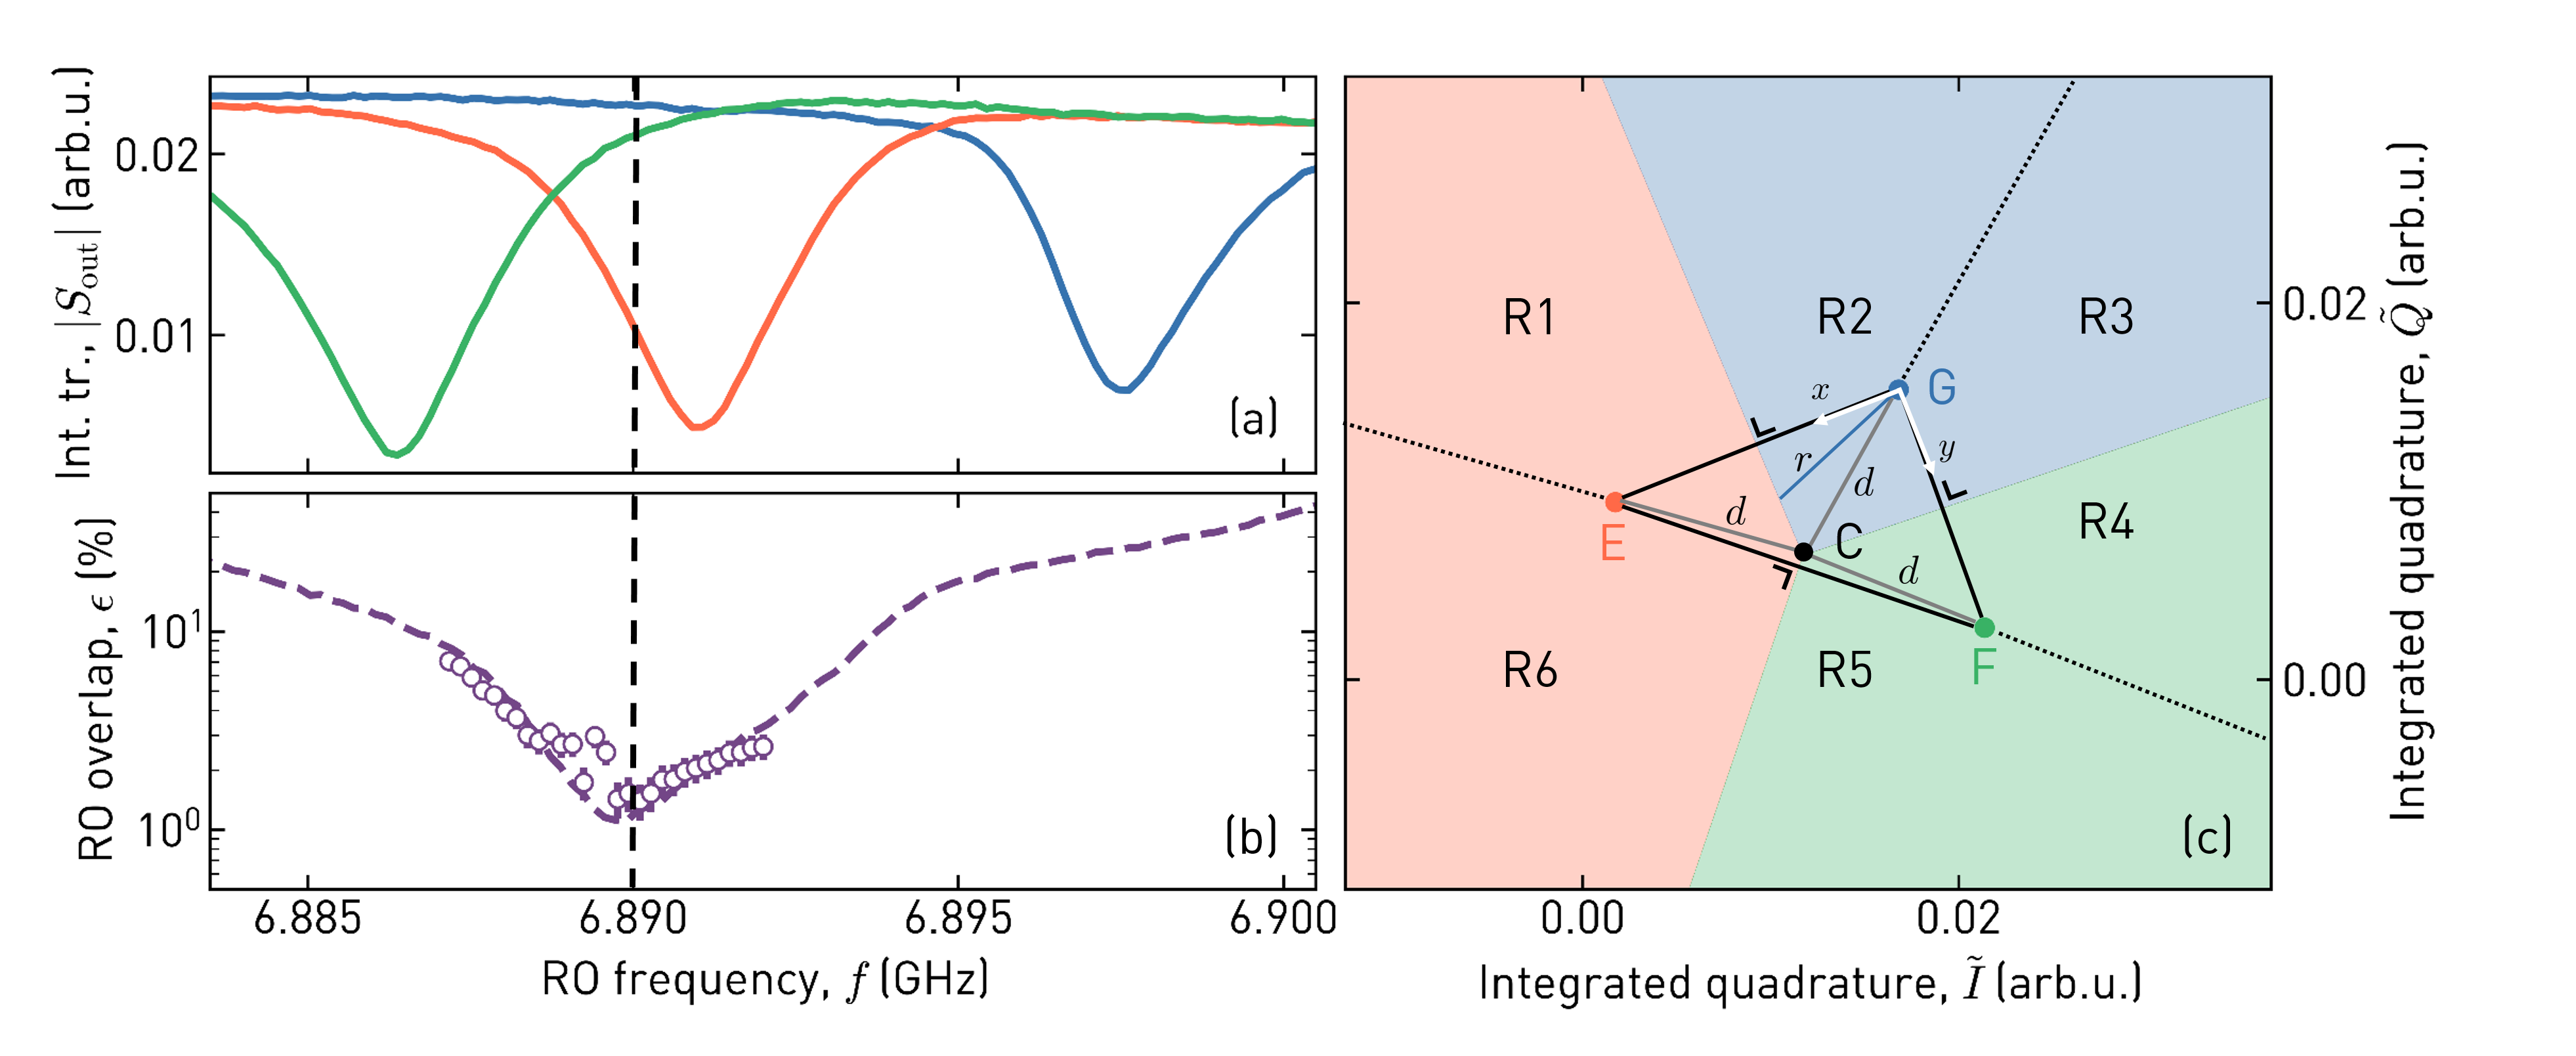
\includegraphics[width=\textwidth]{appendices/qutrit_readout/figs/ch3_readout_frequency_opt__with_iq_20200301_174851_ppt.png}
    \caption{Readout frequency optimization. (a) Amplitude of the integrated state-dependent resonator response (i.e. transmission) for qubit 2 prepared in \g{} (blue), \e{} (red), \f{} (green). (b) Average readout overlap (in \%) as predicted from the model (dashed line) and measured (scatter). (c). Integrated IQ-plane for $f = 6.890\unit{GHz}$ (dashed line in (a),(b)), the frequency for which the readout overlap is minimal. Points $G$, $E$, $F$ correspond to the average integrated resonator responds for states \g,\e{} and \f.  The shaded background color indicates which state is most likely according to a Gaussian mixture model with means centered in $G$, $E$ and $F$, and equal and isometric covariance. $R_i$ indicates different integration regions.  $C$ and $d$ indicate the circumcenter and circumradius respectively. }
    \label{fig:qutrit_readout_ro_freq_opt}
\end{figure}

In the case of equal and isometric covariance of the three distributions, for any measured data point, the distribution with the nearest mean (i.e. vertex of the triangle $GEF$) is the most likely distribution to have generated the data point. In addition, the decision boundaries coincide with the perpendicular bisectors of the triangle $GEF$\footnote{the perpendicular bisectors of a triangle are the collections of points for which the Eucledian distance to two vertices is equal.} (See Fig.~\ref{fig:qutrit_readout_ro_freq_opt}(c)).

Hence,  we compute the readout overlap $\epsilon_k$ consisting of the overlap between the 3 Gaussian distributions (one for each state) at each frequency $f_k$. The frequency yielding the smallest overlap between the Gaussian distributions results in highest \gls{snr} for all three states concurrently and is therefore chosen as readout frequency.

In the next section, we derive an analytical model to find the optimal readout frequency from the average time-integrated resonator responses and discuss the comparison between the model and experimental data shown in Fig.~\ref{fig:qutrit_readout_ro_freq_opt}(b).
 
\subsection{Analytical derivation} \label{s:analytical_derivation_3_gaussians}
We denote the state assignment probability matrix $A_k$ as function of the readout frequency $f_k$ and define the following variables,
\begin{itemize}
    \item[--] $ \mathcal{N}_i^{(k)}(\bm{x}|\bm{\mu}_i^{(k)}, \sigma^2\bm{I}) = \frac{1}{2\pi| \sigma^2\bm{I}|^{1/2}} \cdot \exp\left(-(\bm{x}-\bm{\mu}_i^{(k)})^T\, (\sigma^2\bm{I})^{-1}\,(\bm{x}-\bm{\mu}_i^{(k)})\right)$ the Gaussian distribution modeling measurement noise around state $s_i$ in the two-dimensional integrated IQ-plane at frequency $f_k$.
    \item[--] $\bm{\mu}_i^{(k)}$ the mean of the Gaussian distribution around state $s_i$ at frequency $f_k$, i.e. point $G$, $E$ and $F$ in Fig.~\ref{fig:qutrit_readout_ro_freq_opt}(c) for states \g, \e, \f{} at frequency $f_k = 6.890 \unit{GHz}$.
    \item[--] $\sigma^2\bm{I}$ the equal and isometric covariance of the Gaussian distribution.
    \item[--] $\bm{x}$ an arbitrary point $\in \R^2$ (for ease of notation, we translated the complex IQ-plane to a real, two-dimensional plane).
\end{itemize}

Based on Eq.~\eqref{eq:qutrit_readout_overlap}, the average readout overlap $\epsilon_{k}$ at frequency $f_k$ is, 
\begin{equation}
\epsilon_{k}= \frac{1}{3}\sum_{i=0}^{2}{\sum_{j \neq i}^{2}{P_k(s_j | s_i)}}
\end{equation}
where $P_k(s_j|s_i)$ is the probability of assigning a measurement to state $j$ while it was originally prepared as state $i$ at frequency $f_k$, with $j\neq i$. 

The minimization of the readout overlap is equivalent to a maximization of the trace of $A_k$ over all frequencies, such that finding the optimal readout frequency results in solving,
\begin{equation} \label{eq:opt_freq_proba}
f_{\mathrm{opt}} = \argmax_{f_k} \mathrm{Tr\left(A_k\right)} = \argmax_{f_k} \sum_{i=0}^2{P_k(s_i|s_i)}
\end{equation}

At each frequency, the probability $P(s_i|s_i)$ (we omit $k$ for clarity in the following equations) corresponds to the integral of the Gaussian density function $\mathcal{N}_i(\bm{x}|\bm{\mu}_i, \sigma^2\bm{I})$ over the domain where the density $i$ is higher than the density of any other state. Namely, the area of the two-dimensional IQ-plane in which an incoming point $\bm{x}$ will be correctly assigned $s_i$ if it was prepared in $s_i$. The integration domain are depicted in blue, red, green in Fig.~\ref{fig:qutrit_readout_ro_freq_opt}(c), for state \g, \e, and \f{} respectively.  The optimal readout frequency corresponds to the frequency yielding the largest sum of 3 similar integrals (one for each state)\footnote{For the readout of a two-level system, there are only two integrals and the approximation of equal and isometric covariance allows to ignore one more dimension using an appropriate rotation. The problem reduces to minimizing the overlap between two, one-dimensional Gaussian distributions, which is inversely proportional to the distance between the two means. Hence, the typical choice of readout frequency is the frequency yielding the largest difference between the two state responses~\cite{Heinsoo2018}.}. 

For ease of computation, each integration domain is further divided in 2 sub-domains. By symmetry, 
\begin{subequations}
\begin{equation}\label{eq:I1_integral}
    \int_{R1}{\mathcal{N}_0(\bm{x}|\bm{\mu}_0, \sigma^2\bm{I})\d\bm{x}} = \int_{R2} \mathcal{N}_2(\bm{x}|\bm{\mu}_2, \sigma^2\bm{I})\d\bm{x} = I_1 
\end{equation}
\begin{equation}
\int_{R3}{\mathcal{N}_2(\bm{x}|\bm{\mu}_2, \sigma^2\bm{I})\d\bm{x}} = \int_{R4} \mathcal{N}_0(\bm{x}|\bm{\mu}_0, \sigma^2\bm{I})\d\bm{x} = I_2 
\end{equation}
\begin{equation}
\int_{R5}{\mathcal{N}_2(\bm{x}|\bm{\mu}_2, \sigma^2\bm{I})\d\bm{x}} = \int_{R6} \mathcal{N}_1(\bm{x}|\bm{\mu}_1, \sigma^2\bm{I})\d\bm{x} = I_3 
\end{equation}
\end{subequations}
such that only 3 of the 6 sub-domain integrals need to be computed\footnote{ Note that additional weighting factor to the 3 integrals in this equation allow to favor \gls{snr} of 1 or 2 of the 3 states.},
\begin{equation}
\sum_{i=0}^2{P(s_i | s_i)} = 2 \cdot ( I_1 + I_2 + I_3) \label{eq:total_non_overlap}
\end{equation}

We provide a detailed derivation for $I_1$. The other two integrals are solved in the similar way but are preceded by an appropriate rotation and translation of the coordinate system. 

We start by a shift of coordinate system with the origin at point $G$ and the x-axis aligned with the line segment $|GE|$ such that $\mu_0 = 0$ (see white coordinate system in Fig.~\ref{fig:qutrit_readout_ro_freq_opt}(c)), followed by a polar coordinate transformation. In this parametrization, the radius of integration $r$ is a function of $\theta$, the angle between the x-axis of the coordinate system centered in point $G$ and $r$. Namely,
\begin{equation}
r(\theta) =\begin{cases}
    m / \cos \theta, & \text{if $-\pi/2<\theta<\pi/2$}.\\
    +\infty, & \text{otherwise}.
  \end{cases} 
\end{equation} 
with $m$ being the distance between $G$ and the midpoint of ($G$, $E$), and assuming $\theta \in [-\pi, \pi[$. The integration bounds of $\theta$ are $ \pi - \gamma$ and $\gamma$ where $\gamma = \arccos{d/m}$.

Eq.~\eqref{eq:I1_integral} becomes in the new coordinate system
\begin{equation}
I_1 = \int_{R2} \frac{1}{2\pi \sigma^2} e^{-\frac{\bm{x}^\intercal \bm{x}}{2 \sigma^2}} \d\bm{x}
\end{equation}
and in polar coordinates with the corresponding integration boundaries, 
\begin{equation}\label{eq:qutrit_integral_polar}
I_1=\begin{cases}
    \int_{\gamma - \pi}^{\gamma}\int_0^{m/\cos \theta}{\frac{1}{2\pi \sigma^2} \exp{\left(-\frac{\rho^2}{2 \sigma^2}\right)}\, \rho \,\d\rho \,\d\theta}, & \text{if $-\pi/2<\theta<\pi/2$}.\\
    \int_{\gamma - \pi}^{\gamma}\int_0^{\infty}{\frac{1}{2\pi \sigma^2} \exp{\left(-\frac{\rho^2}{2 \sigma^2}\right)}\,\rho \,\d\rho \,\d\theta}, & \text{otherwise}.
  \end{cases}
\end{equation}
We note that the inner integral in both cases is the derivative of a Gaussian (up to a constant),
\begin{equation}
\int_0^{a}{\frac{1}{2\pi \sigma^2} \exp{(-\frac{\rho^2}{2 \sigma^2})}\rho \,\d\rho \,\d\theta} =\frac{1}{2\pi} \left(1 - \exp{\left(\frac{-a^2}{2\sigma^2}\right)}\right)
\end{equation}
and therefore simplify Eq.~\eqref{eq:qutrit_integral_polar} to
\begin{equation}
I_1 =
\begin{cases}
    \int_{\gamma - \pi}^{\gamma}{\frac{1}{2\pi} \left(1 - e^{-\frac{m^2}{2 \sigma^2 \cdot \cos^2{\theta}}}\right)\,\d\theta}, & \text{if $-\pi/2<\theta<\pi/2$}.\\
    \int_{\gamma - \pi}^{\gamma}{\frac{1}{2\pi}\d\theta}, & \text{otherwise}.
  \end{cases}
\end{equation}

Since $\int_{\gamma - \pi}^{\gamma}{\frac{1}{2\pi}\d\theta}$ is independent of both $\theta$, it results in a constant function integrated over $\pi$. This simplifies $I_1$ further,
\begin{equation} \label{eq:final_frequency_I_integral}
    I_1 = \frac{1}{2} - 
    \begin{cases}
    \int_{\gamma - \pi}^{\gamma}{e^{-\frac{m^2}{2 \sigma^2 \cdot \cos^2{\theta}}}\,\d\theta}, & \text{if $-\pi/2<\theta<\pi/2$}.\\
    0, & \text{otherwise}.
  \end{cases}
\end{equation}
The 0 values for $\theta$ prevent the remaining integral to have a closed form solution, but it can easily be computed numerically. 

An analogous development holds for $I_2$ and $I_3$ for each frequency, the average overlap yields,
\begin{equation} \label{eq:qutrit_ro_overlap_from_integral}
    \epsilon_k = 1 - \frac{2}{3}\cdot \sum_{i=1}^{3}{I_{i,k}}
\end{equation}
and the optimal readout frequency is extracted as defined in Eq.~\eqref{eq:opt_freq_proba},
\begin{equation} \label{eq:optimal_freq}
    f_{\mathrm{opt}} = \argmax_{f_k} {\sum_{i=1}^{3}{I_{i,k}}}
\end{equation}

In Fig.~\ref{fig:qutrit_readout_ro_freq_opt}(b), we show the readout overlap $\varepsilon = \epsilon\cdot 100\%$ computed with Eq.~\eqref{eq:qutrit_ro_overlap_from_integral} for the integrated resonator responses of Fig.~\ref{fig:qutrit_readout_ro_freq_opt}(a) with a dashed, purple line. The minimum average overlap is $~1\unit{\%}$ at $f_{\mathrm{opt}} = 6.890\unit{GHz}$ (dashed black line). 

\subsection{Comparison to experimental data}
We validate the model by experimentally sweeping the readout frequency, recording 20000 single-shot measurements for each eigenstate, and assigning the shots to reconstruct $A_k$ near the frequency of interest. The total (average) experimental error is $1-\mathrm{Tr}\left(A_k\right)/3$. However, the latter includes not only readout overlap errors, but also errors originating from \t{1}-decay and thermal population. Therefore, we use preselection on the single-shot measurements to mitigate the effect of thermal population (see Appendix \ref{app:setup}). To account for errors expected from \t{1}-decay for levels \e{} and \f, we subtract $1-\exp{\left(-t/T_1^{ge}\right)}/3$ and $1-\exp{\left(-t/T_1^{ef}\right)}/3$ from the total error, where $t$ is half the readout length (200 ns). We use $T_1^{ge} = 27.7\, \mu s$ which we measured prior to the single-shot measurements and thereby also infer $T_1^{ef} \approx 27.7 / \sqrt{2}\, \mu s$. The estimated readout overlap errors, which we show in scattered points in Fig.~\ref{fig:qutrit_readout_ro_freq_opt}(b), are in good agreement with the model.

To further reduce the errors caused by readout overlap, we describe in the next section the choice of mode-matched integration weights that linearly increase the \gls{snr}. Note that, since the integration is linear, the readout frequency found in this section remains optimal with mode-matched integration weights.

\section{Mode-matched integration weights} \label{s:mode_matched_integration}
With the readout frequency fixed, we define the mode-matched integration weights for single-shot readout. In a two-level system, taking the complex conjugate of the difference between the average ground and excited state responses of the readout pulse as mode-matched filter coefficients is shown to provide near-optimal filter efficiency~\cite{Heinsoo2018, Gambetta2007, Bultink2018}. The mode-matched weighted integration of the time trace $S_{\mathrm{out}}(t)$ is then: 
\begin{equation}
    x_1 = \int_{0}^{T}{w_{1}(t)\cdot S_{\mathrm{out}}(t)\d t} 
\end{equation}
where $w_{1}(t)$ are the mode-matched weights described above. The index specifies that this is the complex weights corresponding to the \textit{first} integration unit.
A second integration unit is defined to extend this scheme to a three-level system~\cite{Reuer2018}. More specifically, the second integration unit and corresponding weights, $w_2(t)$, are chosen such that $\{w_{1}(t), w_{2}(t)\}$ is a basis spanning the hyper-plane defined by the average response of the three states. Similarly to the two-level case, $w_{2}(t)$ corresponds to the complex conjugate of the difference between the average ground and \textit{second} excited state responses.

These two sets of complex weights are then uploaded on the \gls{uhf} to perform real-time integration of the time traces, such that each single-shot measurement results in a two-dimensional data point (one for each integration unit), $\bm{x}$, where the integral is replaced by a sum,
\begin{equation}
        x_i = \sum_{t=0}^{T}{w_{i,t}\cdot S_\mathrm{out, t}} \text{ for $i \in \{1,2\}$}
\end{equation}
and the time interval is the sampling rate of the \gls{uhf} (2.4\unit{GHz}).

\section{Characterization of three-level single-shot readout} \label{s:experimental_data}
Three-level single-shot readout has been previously been demonstrated on transmon qutrits~\cite{Kurpiers2018DeterministicPhotons, Magnard2018FastQubit}. This section demonstrates the ability to perform single-shot readout on a transmon with a correct state assignment probability of 98.52\%\footnote{For the comparison between three-level and two-level readout performance on the same qubit, see~\cite{Lacroix2019}.}. To the best of our knowledge, this exceeds other correct state assignment probabilities reported in literature for transmon qutrits. In addition, we describe how to use the readout scheme to characterize the three-level populations in any measurements and illustrate it on the  $T_1$ measurement of the \f-level.

\subsection{Single-shot readout characterization} \label{sec:qutrit_readout_ro_characterization}
We use the following calibration routine to assess the performance of the qutrit readout:
\begin{enumerate}
    \item Calibrate parameters of the $R^{\pi}_x$ rotation pulse to prepare the qubit in state $|e\rangle$. 
    \item Calibrate parameters of the second excitation pulse to prepare the qubit in state $|f\rangle$.
    \item Measure average, time-dependent readout responses of the resonator for each eigenstate with the readout pulse frequency $f_{\mathrm{opt}}$ obtained as described in Section \ref{s:frequency_optimization}. The complex conjugate difference in IQ-plane between the ground and first excited state time-traces is taken as integration weights for the first integration unit. The second is defined by using the Gram-Schmidt algorithm~\cite{Bjorck1994NumericsOrthogonalization} on the complex conjugate difference between the ground and second excited state to find an vector, ortho-normal to the first set of integration weights, and spanning the hyperspace of the 3 eigenstates. 
    \item Upload the two sets of integration weights,  $\{w_1, w_2\}$, to the \gls{uhf} for real-time integration.
    \item Prepare each eigenstate 50000 times\footnote{Empirically found to be a  number of shots achieving low statistical estimation errors.}, which after real-time integration results in a two-dimensional data point per shot.
    \item Fit a \gls{gmm} to the dataset of integrated shots using the expectation maximization algorithm~\cite[p.~434-439]{Bishop2006} with the constraint of equal covariance. 
    \item Assess the readout by constructing the state assignment probability matrix.
\end{enumerate}

We apply this procedure to qubit 1 of the device described in Appendix \ref{app:setup} and present the results in Fig.~\ref{fig:ssro_opt}. The corresponding mode-matched integration weights, as well as the readout parameters optimization are reported in~\cite[Appendix B]{Lacroix2019}.

Predicting the most likely state on the entire 2D-plane results in the decision boundaries indicated by the background color of the experimental data in Fig.~\ref{fig:ssro_opt}(a). These one-dimensional boundaries can be interpreted as the natural extension of the threshold (zero-dimensional) used in a two-level system for assigning a shot to the ground or excited state. 

\begin{figure}[t]
  \centering
    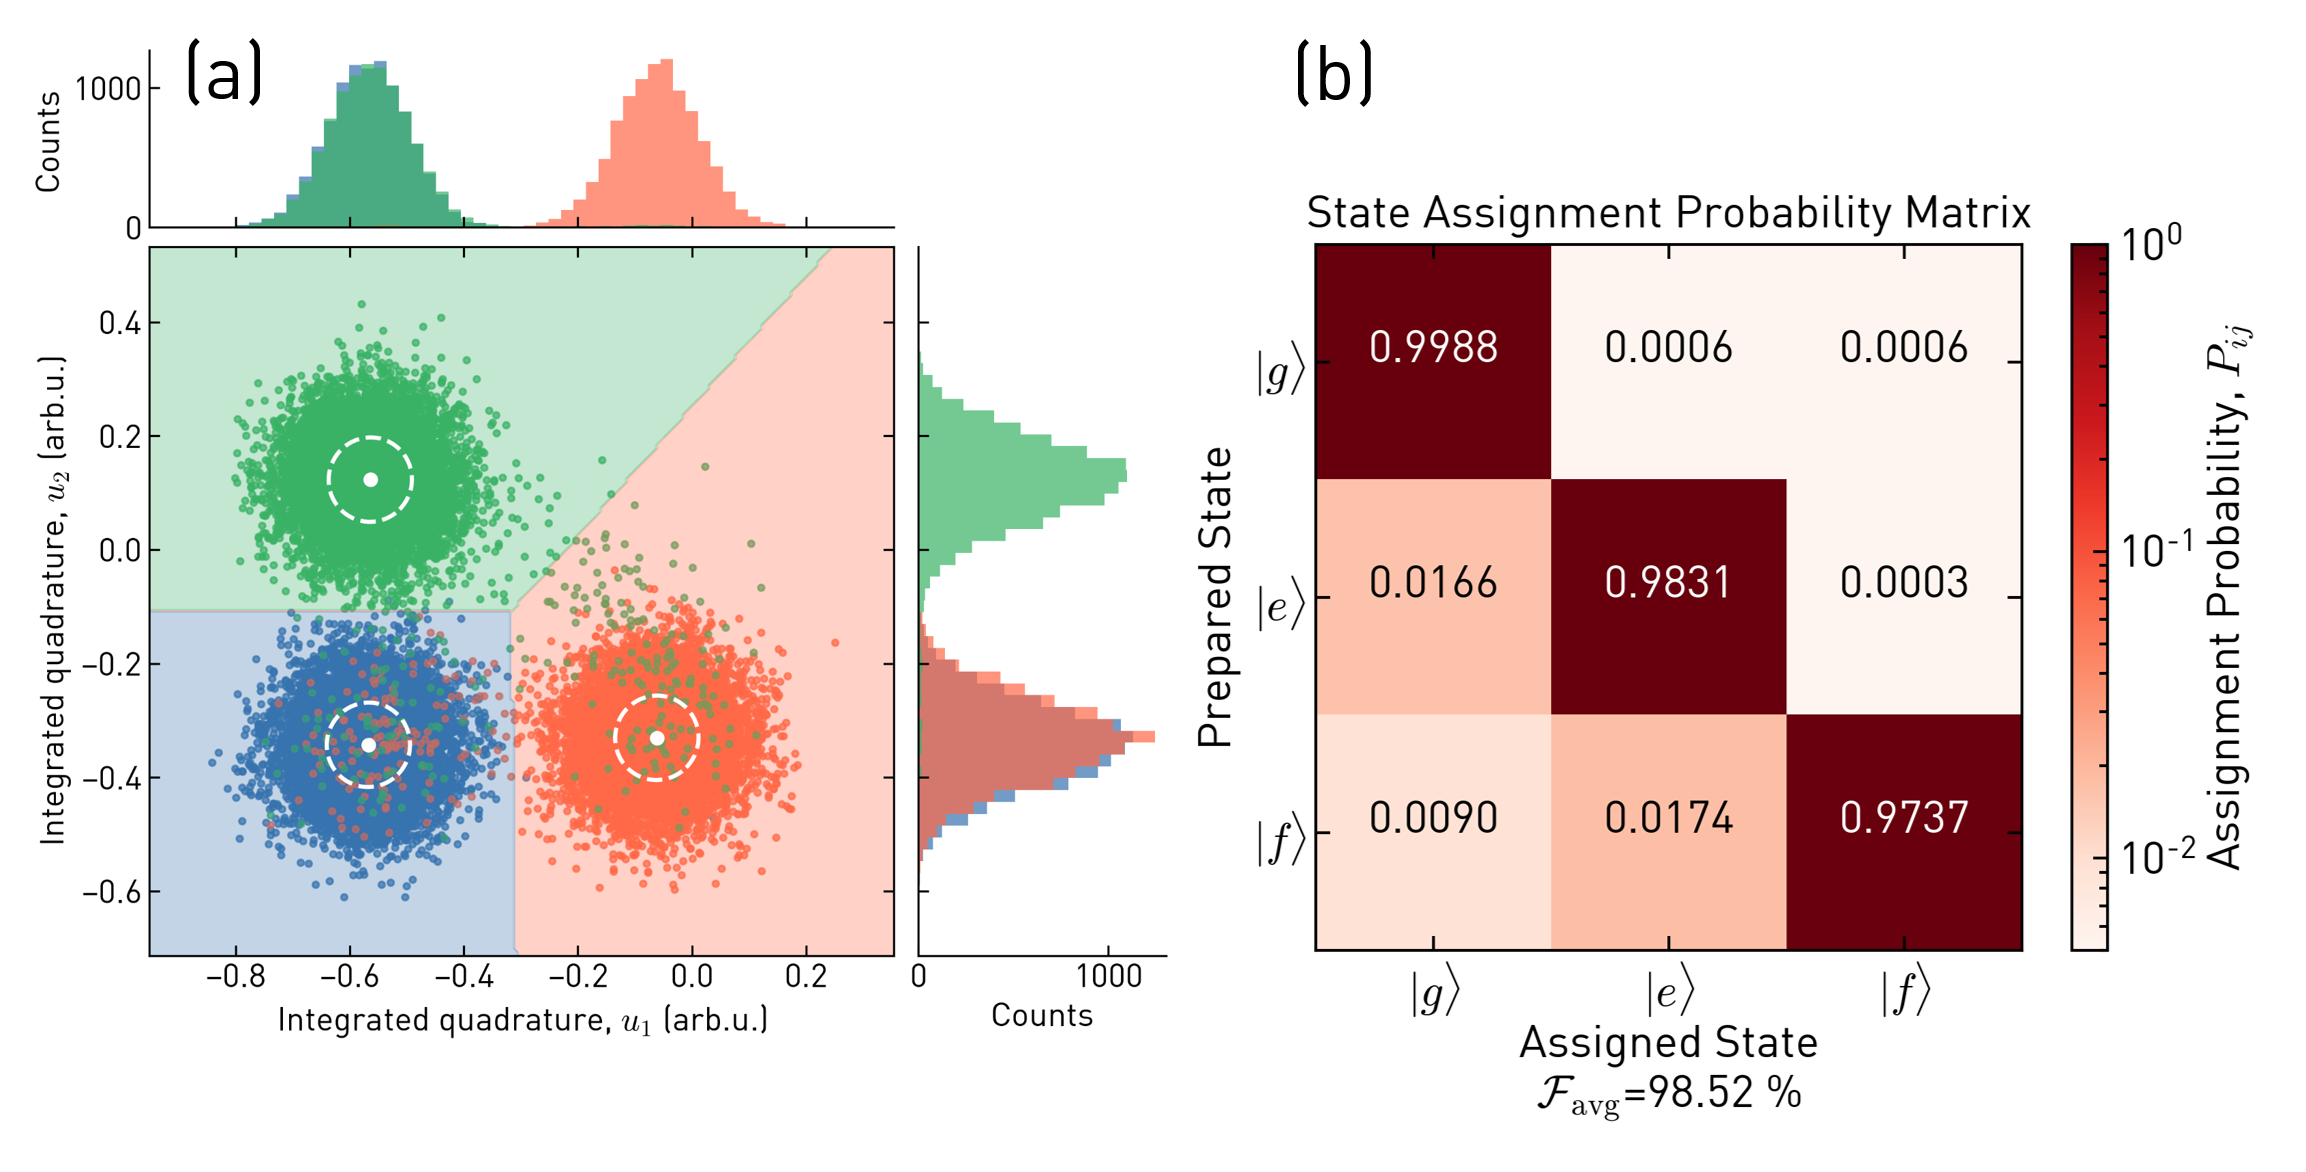
\includegraphics[width=\textwidth]{appendices/qutrit_readout/figs/ch3_readout_GMM_scatter_and_hist_20200116_144401_combined.png}
   \caption{Statistically optimal state assignment with mode-matched integration weights. (a) First 10000 of 50000 single-shot measurements for each eigenstate preparation of qubit 1. Preselection was performed to mitigate thermal population (see Appendix \ref{app:setup} for thermal population estimates). The boundaries correspond to the decision boundaries of the fitted \gls{gmm}. The white points correspond to the position of the means of each Gaussian component and the circle to the standard deviation. In addition, marginal histogram distributions are displayed right and above the main plot. (b) State assignment probability matrix corresponding to the 3x50000 single-shot measurements presented in (a), after pre-selection. The rows correspond to the prepared states and the columns to which state the prepared eigenstates were assigned using the \gls{gmm}.}
  \label{fig:ssro_opt}
\end{figure}

We show the corresponding state assignment probability matrix, $A$, in Fig.~\ref{fig:ssro_opt}(b). The average three-level correct state assignment probability is defined as
\begin{equation}
    \mathcal{F}_{avg} = \frac{1}{3}\mathrm{Tr}(A)
\end{equation}
For the presented run, it amounts to 98.52\%. Notable observations for each matrix row:
\begin{itemize}
    \item $|g\rangle$: Preselection procedure removes the majority of the thermal population (on the order of 1\%, see Appendix \ref{app:setup}). We estimate 0.05\% measurement-induced transition by counting the number of ground-state data points further than 5 standard deviations away from the mean\footnote{Decision boundaries are approximately 3.3 standard deviations away from the mean. The probability that an error is caused by readout overlap is much smaller than by measurement-induced excitation at a distance of 5 standard deviation from the mean.}. remaining errors are caused by the overlap between the distributions.
    \item $|e\rangle$: 
    \begin{itemize}
        \item The assignment of a $|g\rangle$ state for a $|e\rangle$ preparation is dominated by $T_1$-decay. Given a $T_1$ of $25.11\, \mu s$ (last recorded $T_1$) 1.11\% of the prepared $|e\rangle$ shots decay during the first 280\unit{ns} of the readout\footnote{The entire readout is 400\unit{ns} long but only decay events before the first 280\unit{ns} are expected to be misclassified. This corresponds to the time at which 50\% of the information (i.e. integral of the absolute value of mode-matched weights) to distinguish \g{} and \e{} is acquired}. This number explains an important fraction of the observed 1.66\%. 
        The overlap of distributions due to finite \gls{snr} is another source of errors.
        \item The assignment of $|f\rangle$ state for a $|e\rangle$ likely arise from measurement induced transitions, amounting to approximately 0.02\%. Errors originating from readout overlap errors likely explain other errors. 
    \end{itemize}
    \item $|f\rangle$: similarly, misclassification of the $|f\rangle$ state is dominated by $T_1^{ef}$ decay. With a $T_1^{ef}$ of $\sim14.4\, \mu s$,  1.93\% of the initial \f{} population are expected to decay to \e{} or \g. The largest fraction thereof is expected to be classified as $|e\rangle$, while a smaller fraction is expected to have decayed twice during the measurement. The remaining 0.7\% are partially explained by readout overlap errors and preparation errors (which are expected to be higher than \e-level preparation errors because the \f-level preparation requires two pulses).
\end{itemize}

These numbers are summarized in Table \ref{tab:error_mechanisms}. Overall, the error mechanism dominating the state assignment probability matrix is $T_1$- and $T_1^{ef}$-decays, which explain on average 1.01\% of the 1.48\% errors. The total readout overlap error of the Gaussian components, computed using the method described in  \ref{s:analytical_derivation_3_gaussians}, amounts to 0.072\%. Estimated measurement-induced transitions explain on average 0.07\%. Remaining errors amount to 0.33\%, which we suspect are related to fluctuations in $T_1$ and $T_1^{ef}$ as measurement-induced transitions are extremely small on this qubit. This analysis also does not take into account errors originating from leakage into the $\ket{h}$ (or higher) state(s). These errors can lead to misinterpretation of misclassifications of the \f-level in the observed subspace of states $\{\ket{g}, \ket{e}, \ket{f}\}$, depending on where those higher states are projected in the integrated plane. We do observe such effects when optimizing the readout amplitude (see~\cite[Appendix B, Fig.~11]{Lacroix2019}). However, even if not completely negligible, these errors do not impact directly the subspace of interest spanned by $\{\ket{g}, \ket{e}\}$. Indeed, they mostly occur due to measurement-induced transitions on prepared \f-states, which we do not use directly when running quantum algorithms in the computational subspace. 

\begin{table}[ht]
\centering
\caption{Error mechanisms for the measurement displayed in Fig.~\ref{fig:ssro_opt}.}
\begin{tabularx}{0.65\textwidth}{ll}
\toprule 
\textbf{Error mechanism} & \textbf{Error (\%)} \\
\midrule
    $T_1$ and $T_1^{ef}$-decay & 1.01 \\
    Readout overlap & 0.07\\
    Measurement-induced transitions &  0.07 \\
    \midrule
    Total explained errors & 1.15  \\
    \midrule
    Total errors & 1.48 \\
\bottomrule
\end{tabularx}
\label{tab:error_mechanisms}
\end{table}

This analysis suggests that improving the qubits lifetime and/or increasing the readout speed is the most effective way to further increase the correct state assignment probability. In cases where the overlap errors are higher, it might be worth exploring  bi-chromatic readout pulses~\cite{Collodo2020}. Indeed, this method could help increasing the \gls{snr} between the 3 eigenstates, thereby reducing overlap errors. It could also help reducing the readout amplitude, which in turn can contribute reducing measurement-induced leakage. It remains unclear whether the improvements this readout pulse may provide are significant and worth the overhead of calibrating additional parameters.

In summary, we have demonstrated the ability to perform three-level, single-shot readout with an average correct assignment probability superior to 98\% on a transmon qutrit. The assignment errors are dominated by decay events during the 400\unit{ns} readout  originating from the finite lifetime of the \e{} and the \f{} level. In the next section, we detail how to monitor the populations of the first three basis states of a transmon with this readout scheme for arbitrary measurements and illustrate the scheme on a \t{1}-measurement of the \f{} level.

\subsection{Using the three-level readout} \label{sec:qutrit_readout_correction}
After calibration on reference single-shot readout measurements, the \gls{gmm} enables the assignment of state labels to single-shots in any measurement. The fraction of single-shot assigned to each of the state \g, \e{} and \f{} yield (measured) estimates $\bm{P}^m = (P_g^m, P_e^m, P_f^m)^\intercal$ for the populations $\bm{P} = (P_g, P_e, P_f)^\intercal$ of Eq.~\eqref{eq:qutrit_state}~\cite{Magnard2018FastQubit}.

However, as discussed in Section \ref{sec:qutrit_readout_ro_characterization}, the state assignment is sensitive to readout imperfections and therefore yields biased population estimates. For instance, a pure \e{} state measurement should result in $\bm{P}^m = (0,1,0)^\intercal$ but might instead yields $\bm{P}^m = (0.017,0.983,0.0)^\intercal$, just as in the calibration measurement. To account for these imperfections, we use a latent variable model~\cite{Cai2012LatentModeling} to infer the (corrected) qutrit populations $\bm{P}^c$ relative to the calibration measurement,
\begin{equation}
    A^\intercal \cdot \bm{P}^c = \bm{P}^m
\end{equation}
where $\bm{P}^c$ are the latent (corrected) qutrit populations (3x1), $\bm{P}^m$ are the measured qutrit populations and $A$ is the reference state assignment matrix obtained during calibration. To infer $\bm{P}^c$, we multiply the measured population by the transpose inverse of the reference state assignment probability matrix,
\begin{equation} \label{eq:mtx_inversion}
     \bm{P}^c = (A^{\intercal})^{-1} \cdot\bm{P}^m
\end{equation}
where $(A^{\intercal})^{-1}$ can be seen as a linear filter acting on $\bm{P}^m$. 

Note that this procedure assumes that $A$ stays constant over time, which is not evidently fulfilled. For instances, fluctuations in $T_1^{ge}$ and $T_1^{ef}$ directly induce fluctuations in $A$, which can lead to over- or under-correction of the populations. Therefore, a reference matrix $A$ must be recorded at the end of each measurement sequence, similarly to \g{} and \e{} state calibration points typically used in Rabi oscillation measurements. 

In Fig.~\ref{fig:t1ef_3lv}, we display the time evolution of the measured qutrit populations for a $T_1$-measurement of the \f-level. The scattered points, which correspond to the measured populations $\bm{P}^m$, are in excellent agreement with the rate-equation evolution shown in solid lines. The rate-equation accounts for thermal population and its only free the parameter is $T_1^{ef}$, for which we find a value of $14.96 \pm 0.09 \,\mu\textrm{s}$. 

At short time scales, the qutrit is in the second excited state and progressively decays into the first excited state. $P_e^m$ first grows exponentially as $P_f^m$ decays with the time constant of T$_1^{ef}$. After approximately 20 $\mu s$, the decay from the \e-state to the \g-state with time constant T$_1^{ge}$ becomes more important than the remaining incoming population from the \f-level.  This results in a decrease of the \e-level population at larger time scales. The \g-state population is zero at the start of the measurement and increases progressively as the time evolving population of the \e-level decays into the \g-state. The population dynamics in this measurement illustrate that obtaining a good estimate for $T_1^{ef}$ is more intricate without three-level readout because there is no way easy way to detect the cascaded decay without monitoring all states. 

% The readout procedure also provides an accurate estimate of the leakage in the \f-level for operations which are meant to stay in the computational space, such as two qubit gates. The precise monitoring of leakage during two qubit gates calibration ensure the chosen pulse parameters do not result in leakage. 

% As the number of qubits on quantum processors grows, the speed of the calibration also becomes a

\begin{figure}[ht]
  \centering
     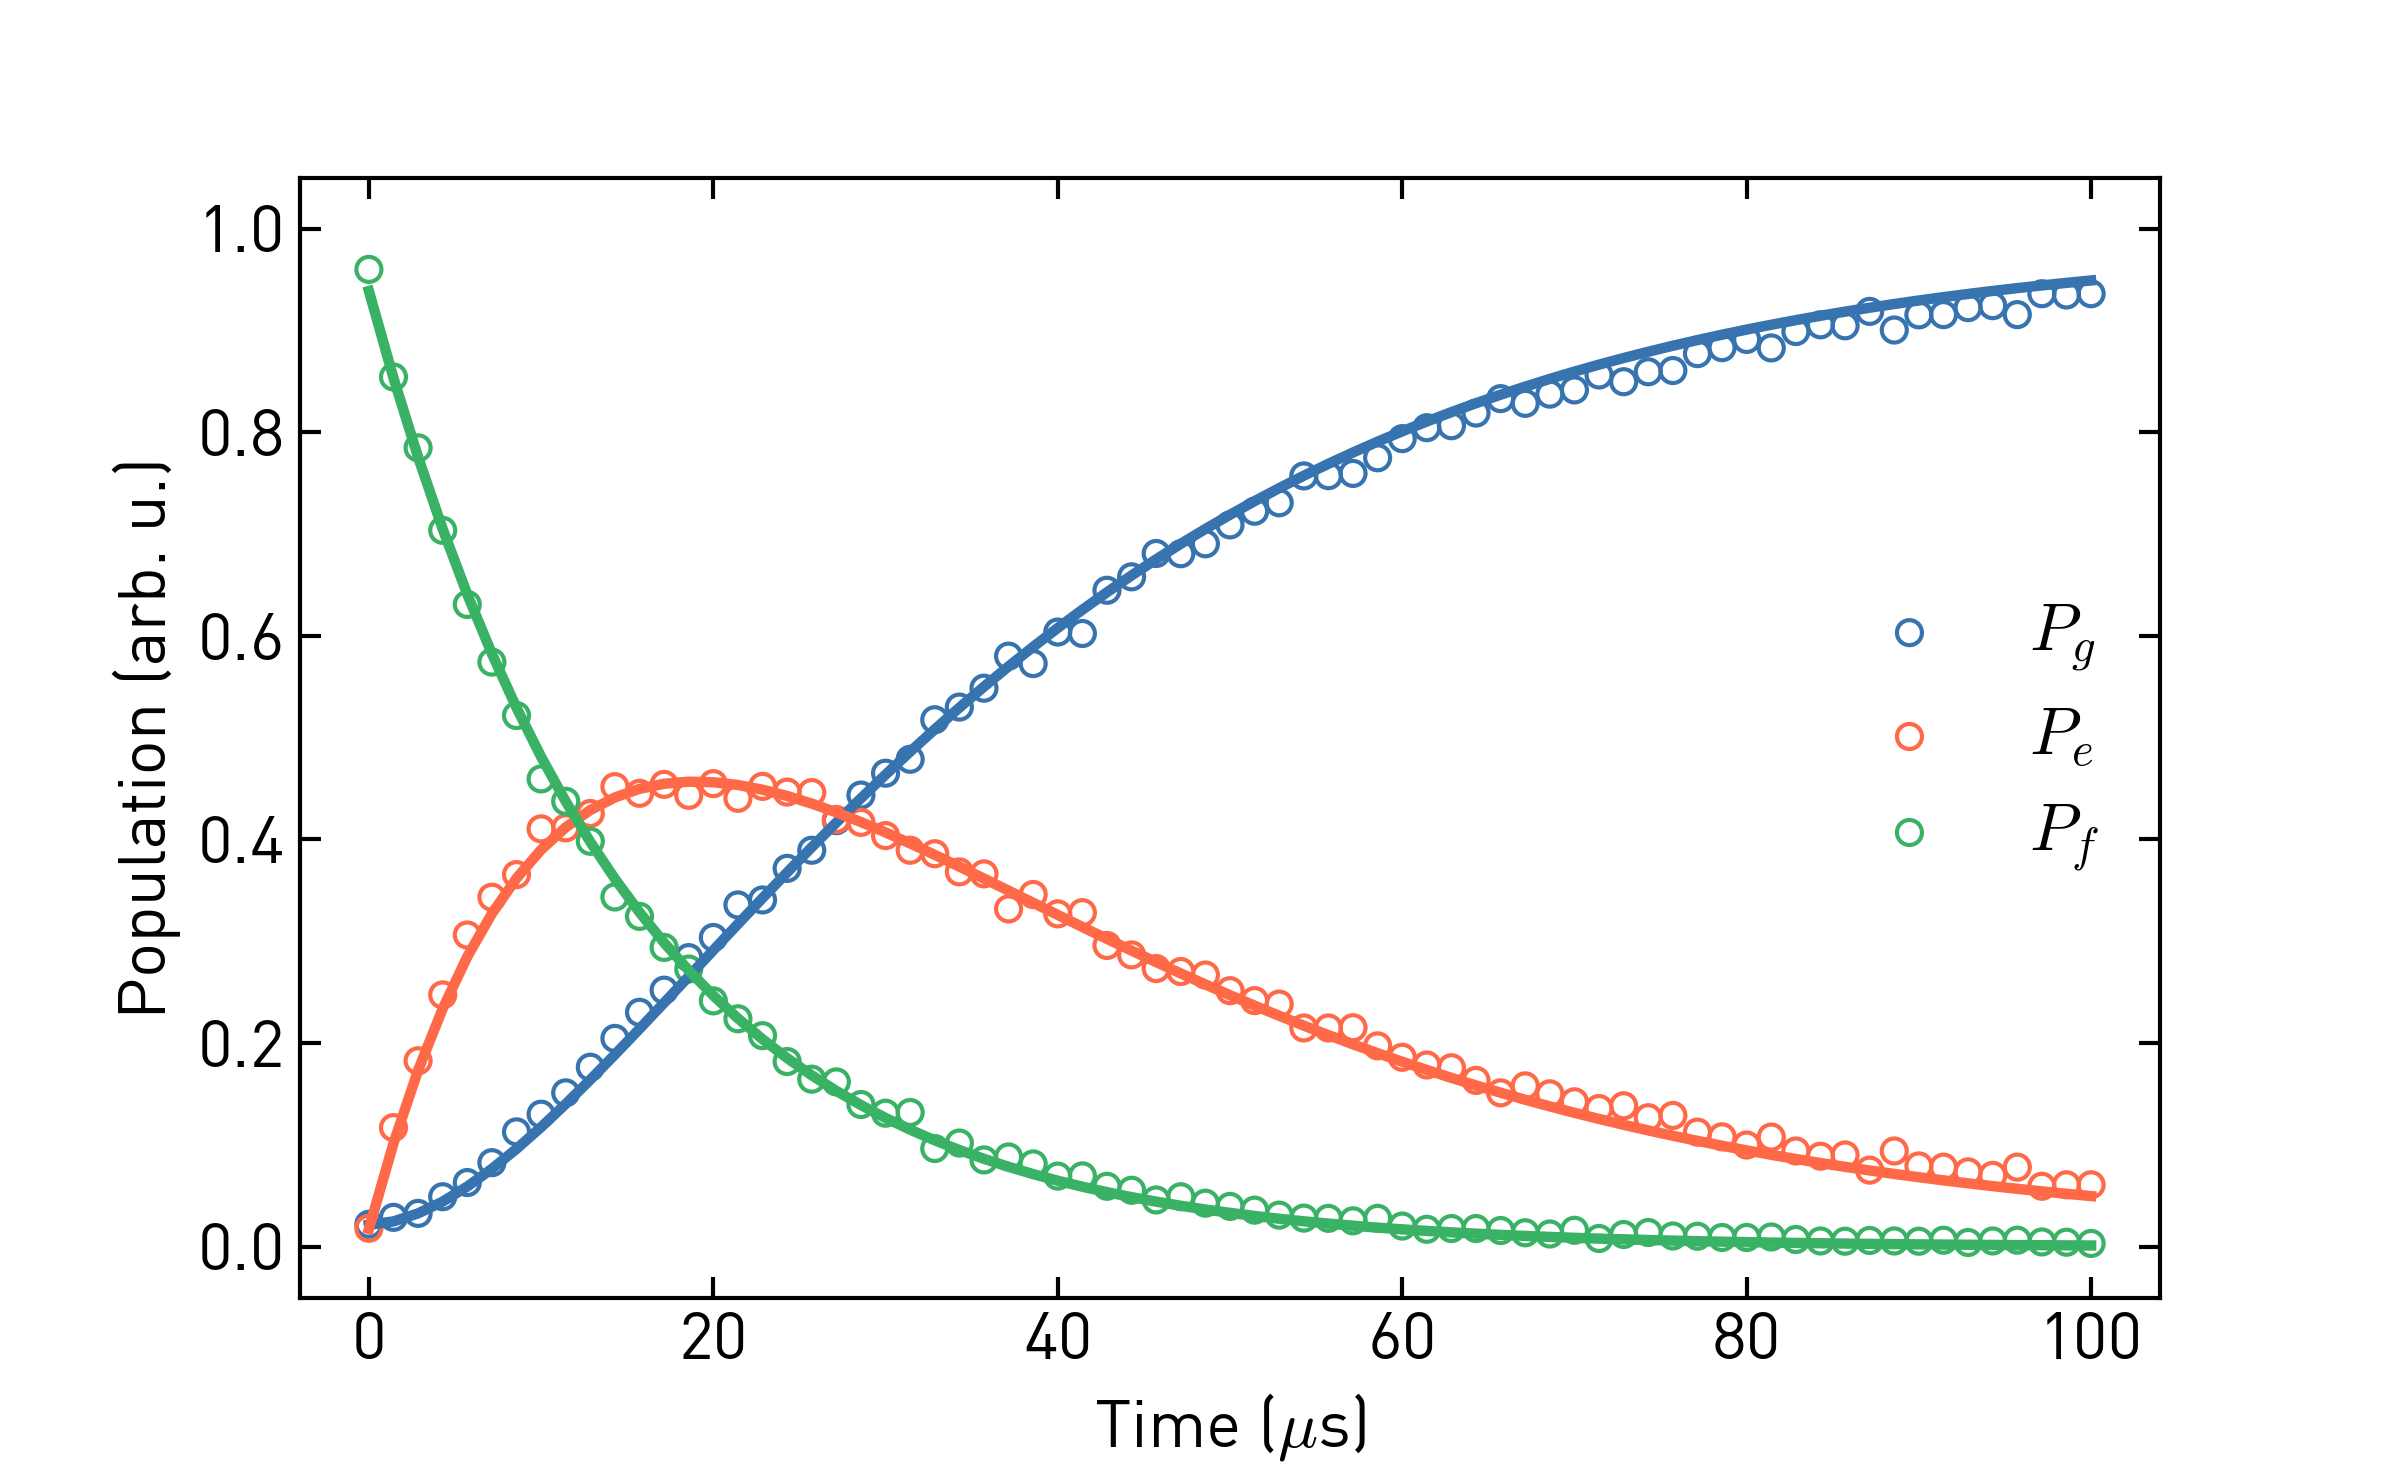
\includegraphics[width=\textwidth]{appendices/qutrit_readout/figs/readout_t1ef_20200302_004024.png}
\caption{Illustration measurements of the three-level readout scheme on qubit 1.  $T_1$ measurement of the \f-level. Time evolution of measured population for each eigenstate (scattered) and population extracted from a rate-equation (solid lines) that accounting for thermal population. We extract a \f-level lifetime of $14.96\, \mu \textrm{s}$.}
\label{fig:t1ef_3lv}
\end{figure}

In the next section, we describe another application of the three-level readout scheme, namely the active reset of a qutrit to its ground state. 

\section{Three-level, measurement-based active reset} \label{sec:active_reset}
Low-latency analysis of quantum states is key for many quantum algorithms, including quantum error correction~\cite{Reed2012RealizationCircuits}, quantum teleportation~\cite{Steffen2013DeterministicSystem}, quantum deep learning~\cite{Cao2017QuantumComputers} and active qubit reset~\cite{Magnard2018FastQubit, Salathe2018Low-LatencyCommunicationb}. These algorithms employ the (assigned) projected state to condition further operations in the quantum circuit. To ensure success of the algorithm, the analysis and feedback operation must occur much faster than the coherence time of the system. 

In this section, we adapt the three-level readout introduced in Section~\ref{s:high_level_description} to perform low-latency state assignment as required for feedback experiments. Next, we use the three-level state assignment in a feedback loop with a transmon to actively reset a qutrit to its ground state. 

\subsection{Setup and procedure for low-latency analysis of quantum states}
We show simplified schematics of our experimental setup in Fig.~\ref{fig:readout_active_reset_schematics}(a) (see Appendix~\ref{app:setup} for detailed schematics). We use Zurich Instruments' \gls{uhf} for readout combined with Zurich Instruments' \gls{hdawg} for drive and feedback pulses generation.

\begin{figure}
    \centering
    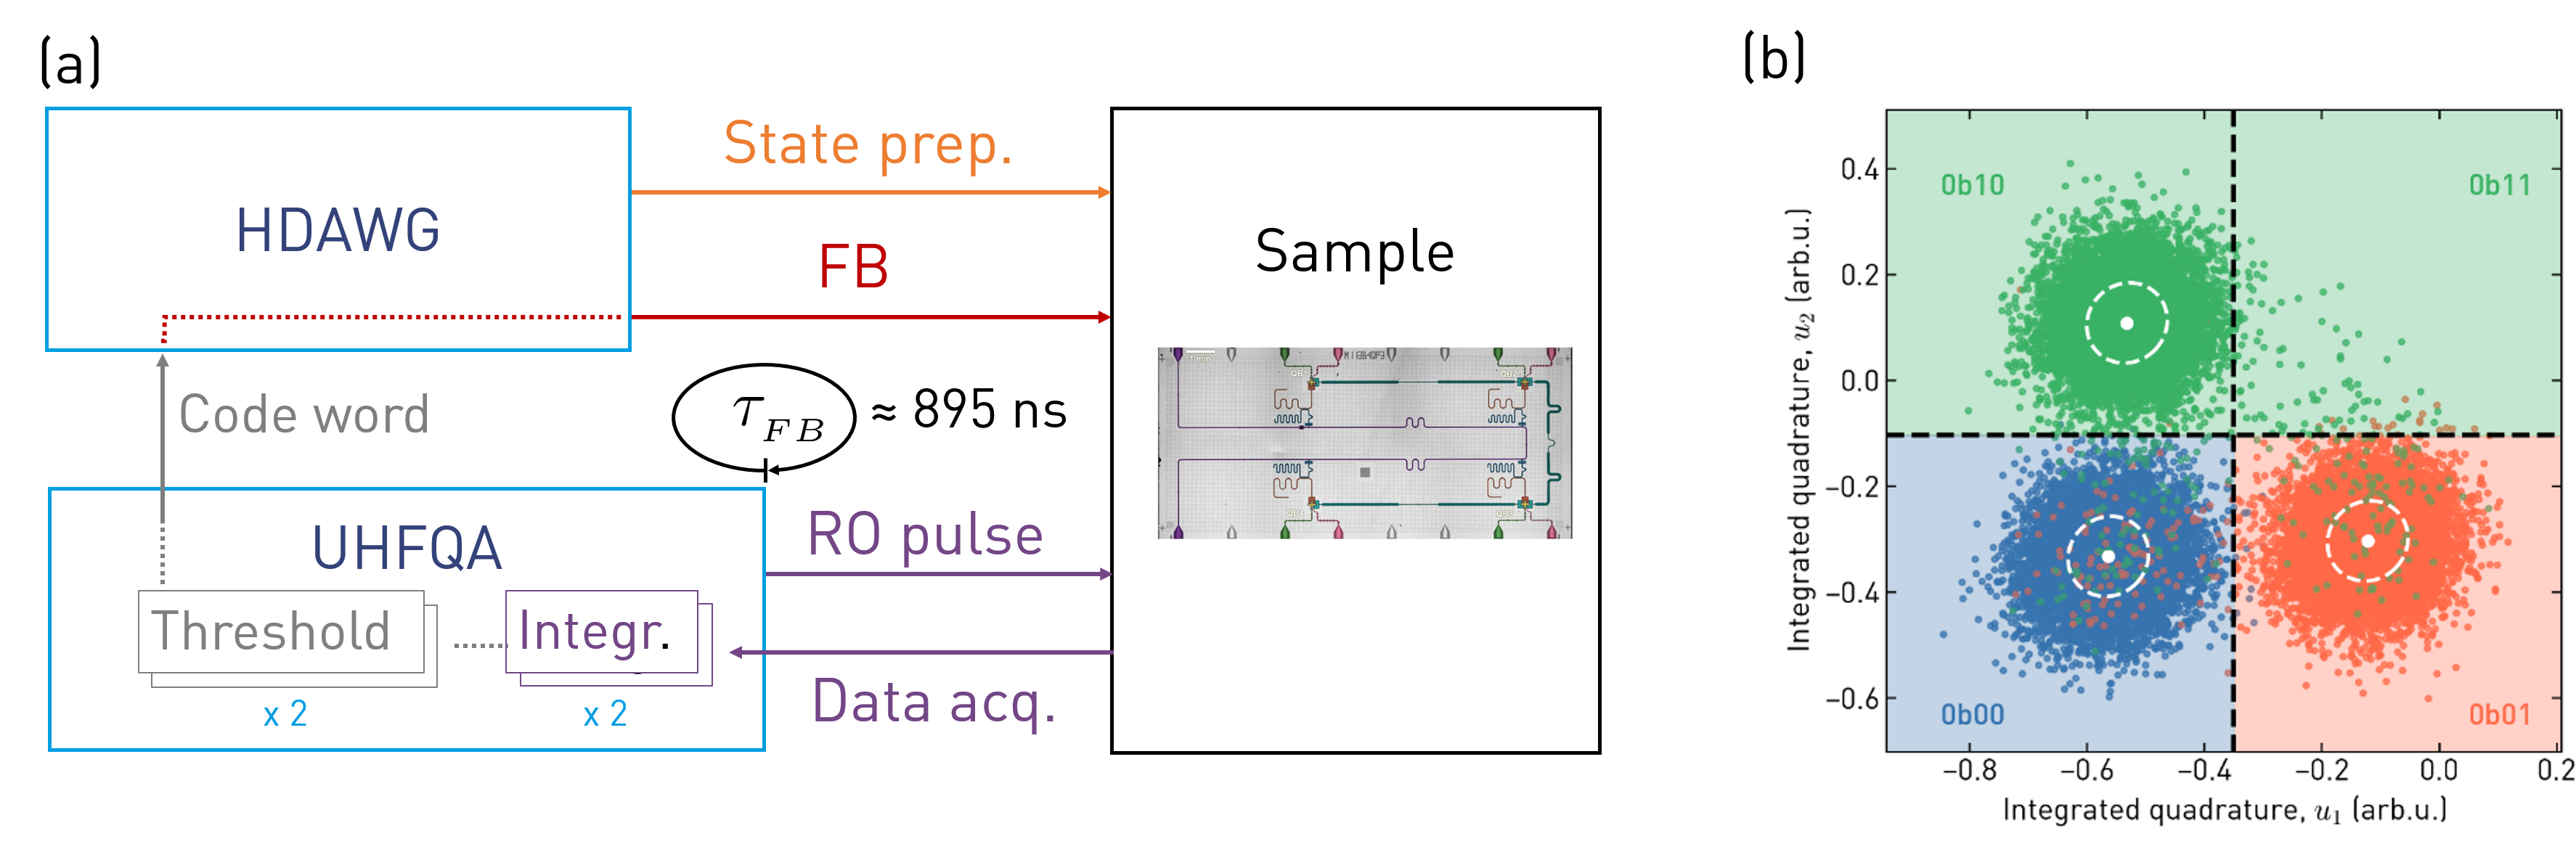
\includegraphics[width=\textwidth]{appendices/qutrit_readout/figs/ch3_readout_active_reset_setup.png}
    \caption{(a) Simplified schematics of the experimental setup: the \gls{hdawg} is used for pulse generation and the \gls{uhf} for readout pulse generation, data acquisition, integration, state assignment, and code word generation. (b) Calibration measurement of the three-level, single-shot readout on qubit 1 to determine the threshold required by the \gls{uhf} for real-time state assignment. The two thresholds are indicated with black, dashed lines. The background color corresponds to the state associated with the code word for each region. The corresponding code words for each regions are displayed in the corners. Blue, red, green correspond to states \g, \e and \f{} respectively. The white dot and circle correspond to the mean and standard deviations of each distribution.}
    \label{fig:readout_active_reset_schematics}
\end{figure}{}

A feedback experiment typically consists of four steps: state preparation, readout, state assignment and feedback operation(s). First, we send microwave pulses generated by the \gls{hdawg} to prepare the quantum state. Next, we send a readout pulse and record the transmission line response with the \gls{uhf}. As described in Section \ref{s:mode_matched_integration}, we integrate\footnote{The \gls{uhf} includes a field programmable gate array (FPGA) that integrates the response in real-time.} the response with mode-matched integration weights yielding a two-dimensional data point for each single-shot measurement. We assign the point to a state in about 400\unit{ns} with predefined thresholds on each integration unit axis, as pictured in Fig.~\ref{fig:readout_active_reset_schematics}(b). We use a decision tree classifier~\cite{Breiman1984} of depth 2 fitted with the CART algorithm~\cite{Breiman1984} to find thresholds on each axis that minimizes the Gini impurity~\cite{Bishop2006, Breiman1984}. In the limit of average \gls{snr} larger than 7, the expected difference in average correct state assignment probability between decision tree classifier and a \gls{gmm} is on the order of $1\permil$ (see~\cite{Lacroix2019} for more details about when this comparison is valid). For the instance presented in Fig.~\ref{fig:readout_active_reset_schematics}(b), the decision tree classifier in fact outperforms the \gls{gmm} by $1\permil$ because it exploits the non-Gaussian distribution of decaying events.
The \gls{uhf} generates binary a two-bit code word (one for each integration channel) defining the location of the data point: the bit is zero if the data point is smaller than the threshold on that axis and 1 if it is larger. The code word is sent over a digital input/output (DIO) port to the \gls{hdawg} that sends different pulses to the device depending on the code word value.

\subsection{Demonstration of three-level active reset}
We use this experimental framework to actively reset a qutrit to its ground state. We characterize the reset procedure for a qutrit prepared in each of the three eigen states with the pulse scheme presented in Fig.~\ref{fig:readout_active_reset_schematics}(a). We prepare the qutrit in \g, \e, or \f{} and then perform $N$ cycles of readout, state assignment and feedback pulses. For each cycle, no pulse is sent to the qutrit if the assigned state is \g. By contrast, if the assigned state is \e{} (\f), single qutrit control pulse(s) $R_{ge}^{\pi}$ ($R_{ef}^{\pi}$ and subsequently $R_{ge}^{\pi}$) are employed to bring the qutrit back to \g. We perform a last readout after the $N$ cycles to characterize the effect of the last feedback pulse.

Each cycle takes approximately 895\unit{ns}; 350\unit{ns} for the readout, 440\unit{ns} for state assignment, code word generation and logical branching in the \gls{hdawg}, 100\unit{ns} to apply the feedback operations  and 5\unit{ns} buffer before the next readout. We fix the time-window reserved for the feedback operations to 100\unit{ns} (which corresponds to the longest possible feedback sequence: two, 50\unit{ns} long single qutrit gates) independently of the assigned state because the state is known only at run time but all triggers are compiled before the start of the measurement.

We present the evolution of the readout-corrected populations $P_{g,e,f}^c$ over time after state preparation in  Fig.~\ref{fig:qutrit_readout_active_reset_populations}(b)-(d).
For reference, we perform the exact same measurement without reset pulses and display the corresponding populations $P_{g,e,f}^{NR}$ with translucent colors. We define the excited state population, $P_\textrm{exc} = 1 - P_g$ and indicate with a red dashed-line the average, steady-state excited population when no reset is applied,
\begin{equation}
    \langle P_{\textrm{exc, ss}}^{NR}\rangle = \frac{1}{N+1}\sum_{n=0}^{N} 1-P_{\textrm{exc},n}^{NR}
\end{equation}
where $P_{\textrm{exc},n}^{NR}$ is the excited state population at the $n$-th readout for a qutrit prepared in \g{}, and $N+1$ is the total number of readouts.

\begin{figure}[ht]
    \centering
    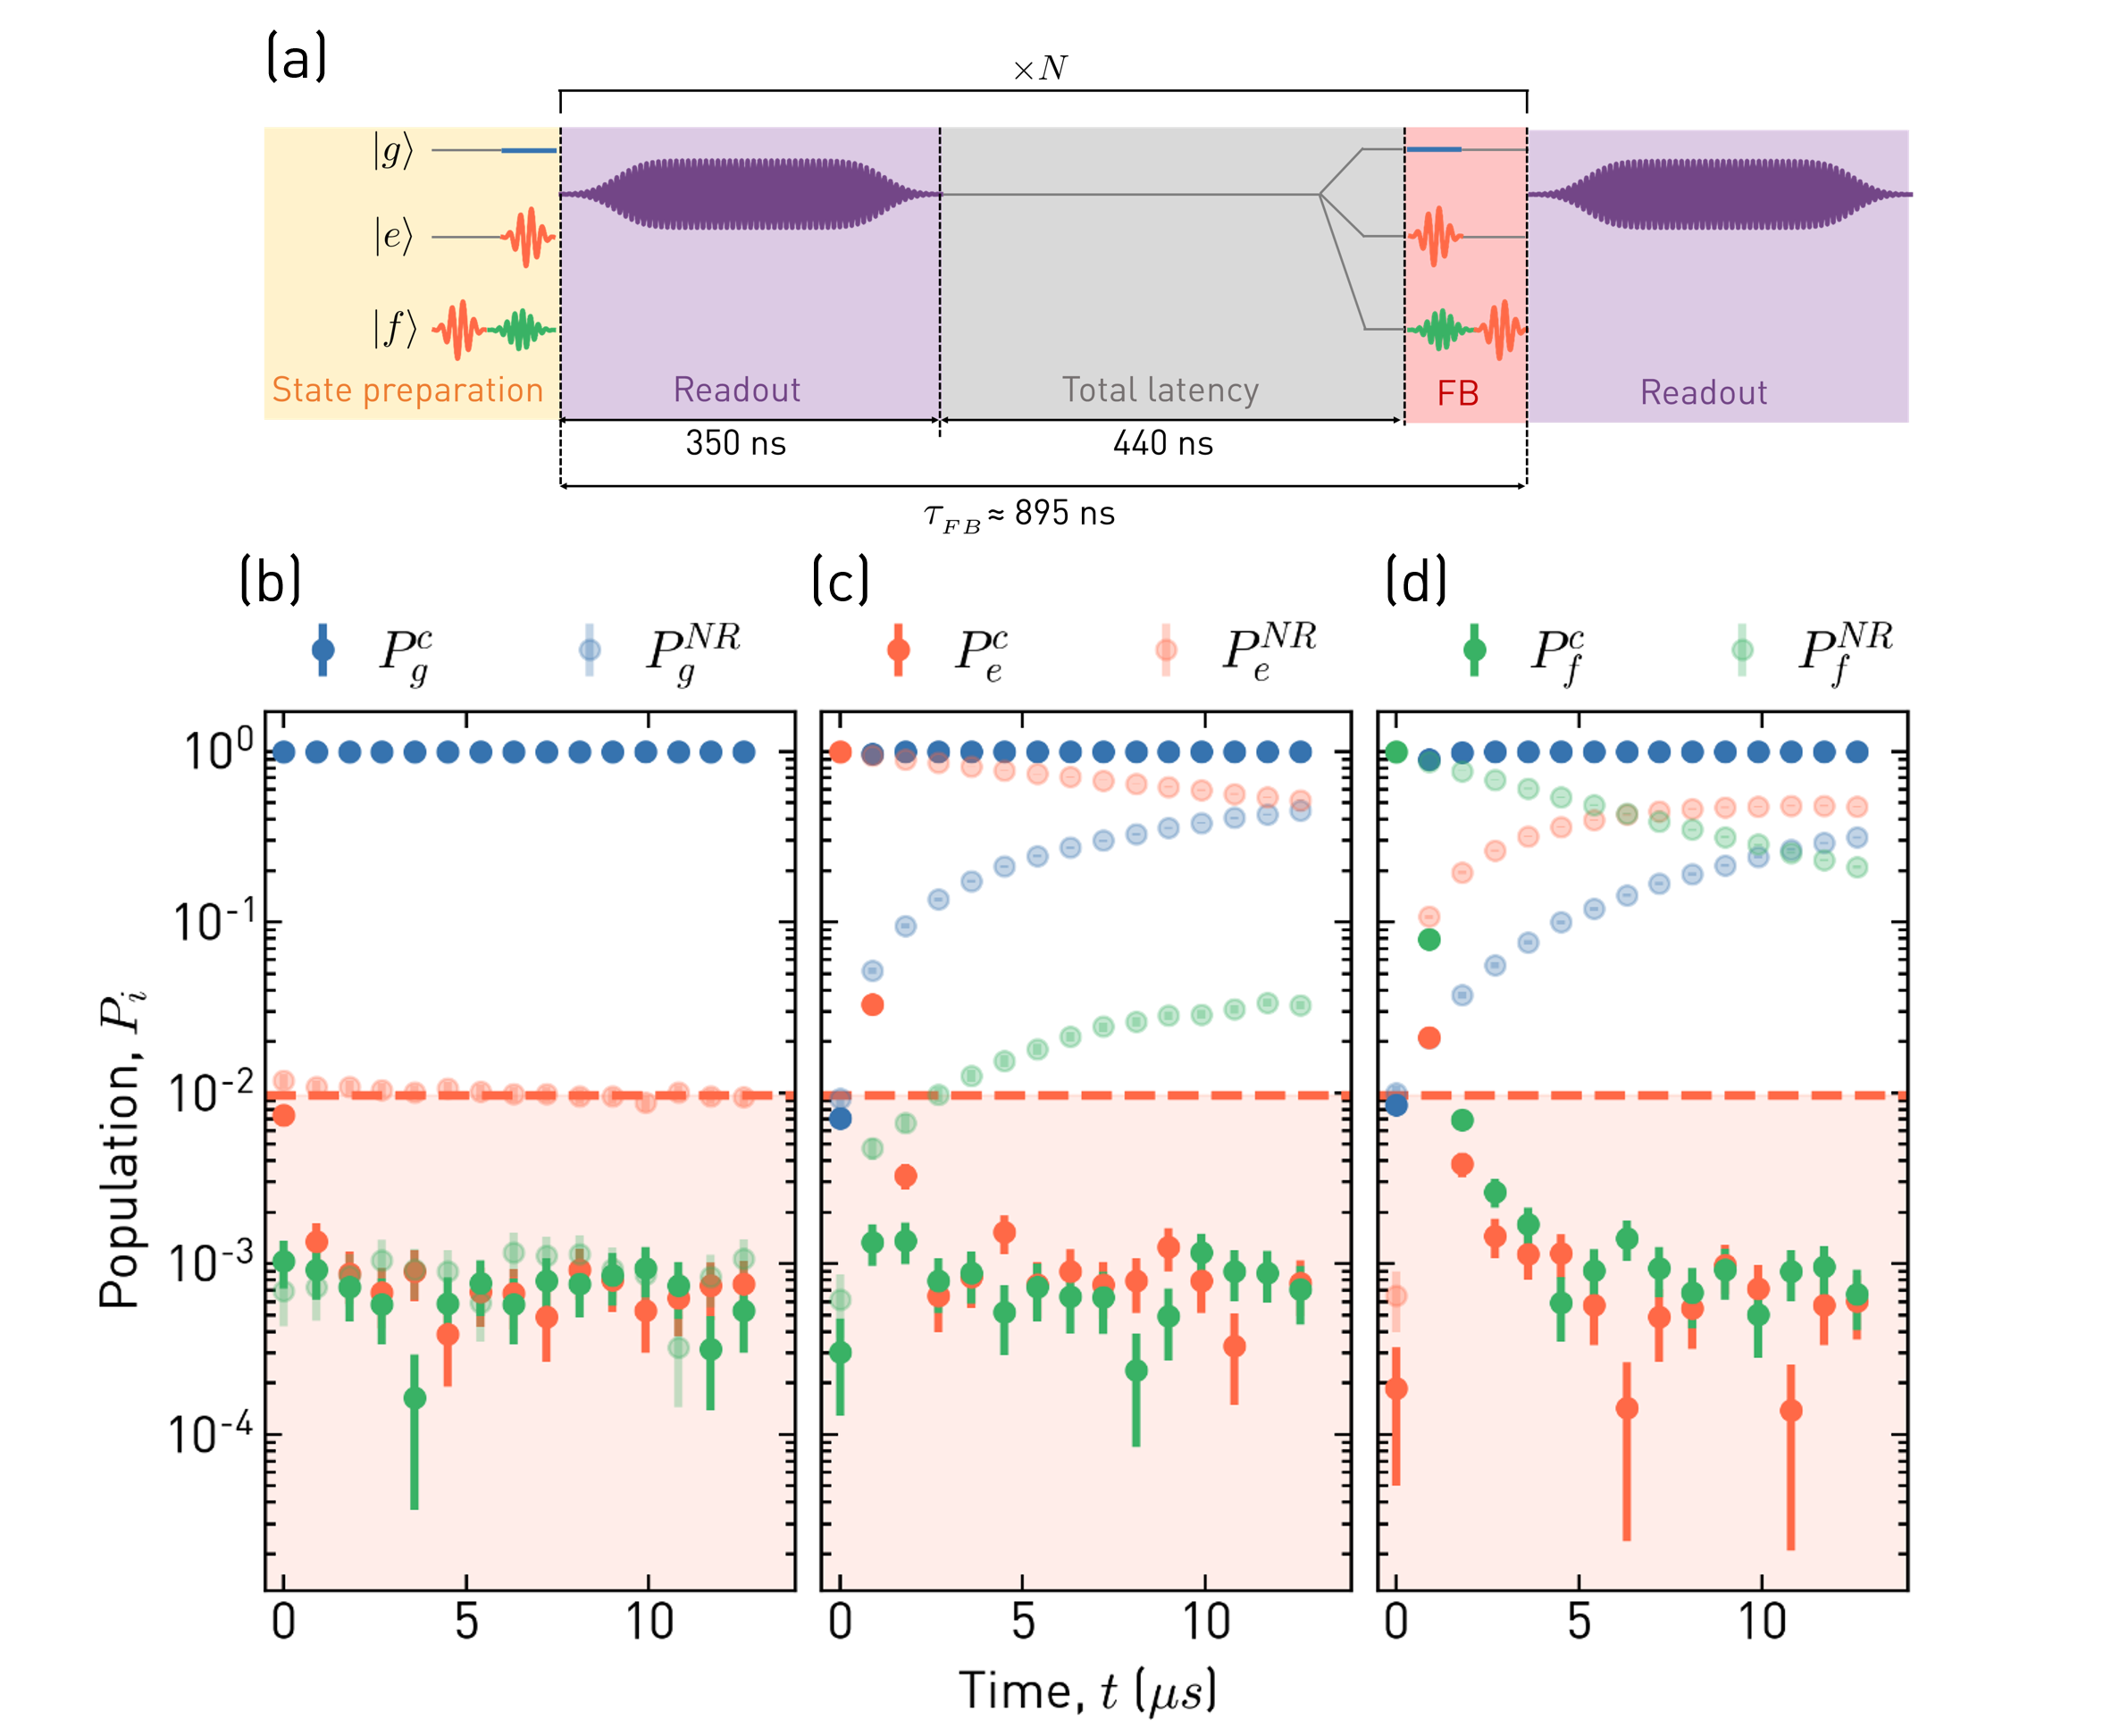
\includegraphics[width=\textwidth]{appendices/qutrit_readout/figs/ch3_readout_active_reset_residual_populations_20200118_175702_with_scheme.png}
    \caption{(a) Pulse scheme used to test the active reset protocol. We prepare a qutrit in one of its eigenstate and subsequently apply $N$ feedback cycles consisting of a readout pulse, a waiting time to assign a state to the acquired data and generate a code word for the \gls{hdawg}, and a feedback sequence to reset the qutrit to the ground state dependent on the code word. Finally, we apply a last readout pulse to evaluate the impact of the last feedback cycle. Single-qubit identity gates $I$ (i.e. wait time) are shown in blue, single-qubit x-rotation in the $ge$-subspace $R_{ge}^{\pi}$ are indicated in red and in red and single-qubit x-rotation in the $ef$-subspace $R_{ef}^{\pi}$ are indicated in green. (b-d) Evolution of the readout-corrected populations $P_{g,e,f}^c$ over time after a state preparation in \g{} (b), \e{} (c) and \f{} (d) of qubit 1. The $n$-th time step corresponds to the $n$-th readout of the reset scheme. The reference measurement recording populations $P_{g,e,f}^{NR}$ without reset pulse is shown with translucent colors in each panel. We indicate the average, steady-state excited population $\langle P_{\textrm{exc}}^{NR}\rangle$ with a dashed red line, and shade the region below this threshold in light red.}
    \label{fig:qutrit_readout_active_reset_populations}
\end{figure}

For a qutrit prepared in \g, about 99\% of the population is measured in \g{} at $t=0$ (i.e. before applying the first feedback pulse), see Fig.~\ref{fig:qutrit_readout_active_reset_populations}(b). The residual excited population originating from thermal excitation amounts to approximately 1\% and is predominantly in the \e-state. After a single feedback cycle, the residual excited population is on the order of $1\permil$, i.e. an order of magnitude smaller, and stays approximately constant thereafter.

Similarly, a qutrit prepared in \e{} starts with approximately 99\% of the population in \e, but requires 2 feedback cycles (1.8\us) to reduce the residual excited population below $\langle P_{\textrm{exc}}^{NR}\rangle$  and 3 cycles (2.7\us) to reach a steady-state of approximately 1.5$\permil$, see Fig.~\ref{fig:qutrit_readout_active_reset_populations}(c). This population transfer occurs about 100 times faster than it would through the natural decay of the qutrit (see translucent data points for comparison). The increase in $P_f^{NR}$ is due to the accumulation of measurement-induced transitions. The ability the readout the \f-state and correct for these excitation results in a constant \f-state population of approximately 1$\permil$ when the feedback is activated.

Finally, we also demonstrate the ability to reset a qutrit prepared in \f{} below $\langle P_{\textrm{exc}}^{NR}\rangle$ with 3 feedback cycles (2.7\us), see Fig.~\ref{fig:qutrit_readout_active_reset_populations}(d).

In Fig.~\ref{fig:qutrit_readout_active_reset_rates}, we present the residual excited state population for a qutrit prepared in \e{} and \f{}, which we fit to a exponential decaying model to extract the reset rate, $\Gamma$, and the residual, steady-state excited population $P_{\textrm{exc}}^{\textrm{ss}}$,
\begin{equation}\label{eq:qutrit_readout_active_reset_rate_model}
    P_{\textrm{exc}} = P_{\textrm{exc}}^{\textrm{ss}} + (1-P_{\textrm{exc}}^{\textrm{ss}}) \cdot \sexp{-2\pi\Gamma t}
\end{equation}

We extract a reset rate of 0.60\unit{MHz} (0.41\unit{MHz}) and a steady-state, residual excited population of 1.5\unit{\permil} (1.7\unit{\permil}) for a qutrit prepared in \e{} (\f). 

\begin{figure}[ht]
    \centering
    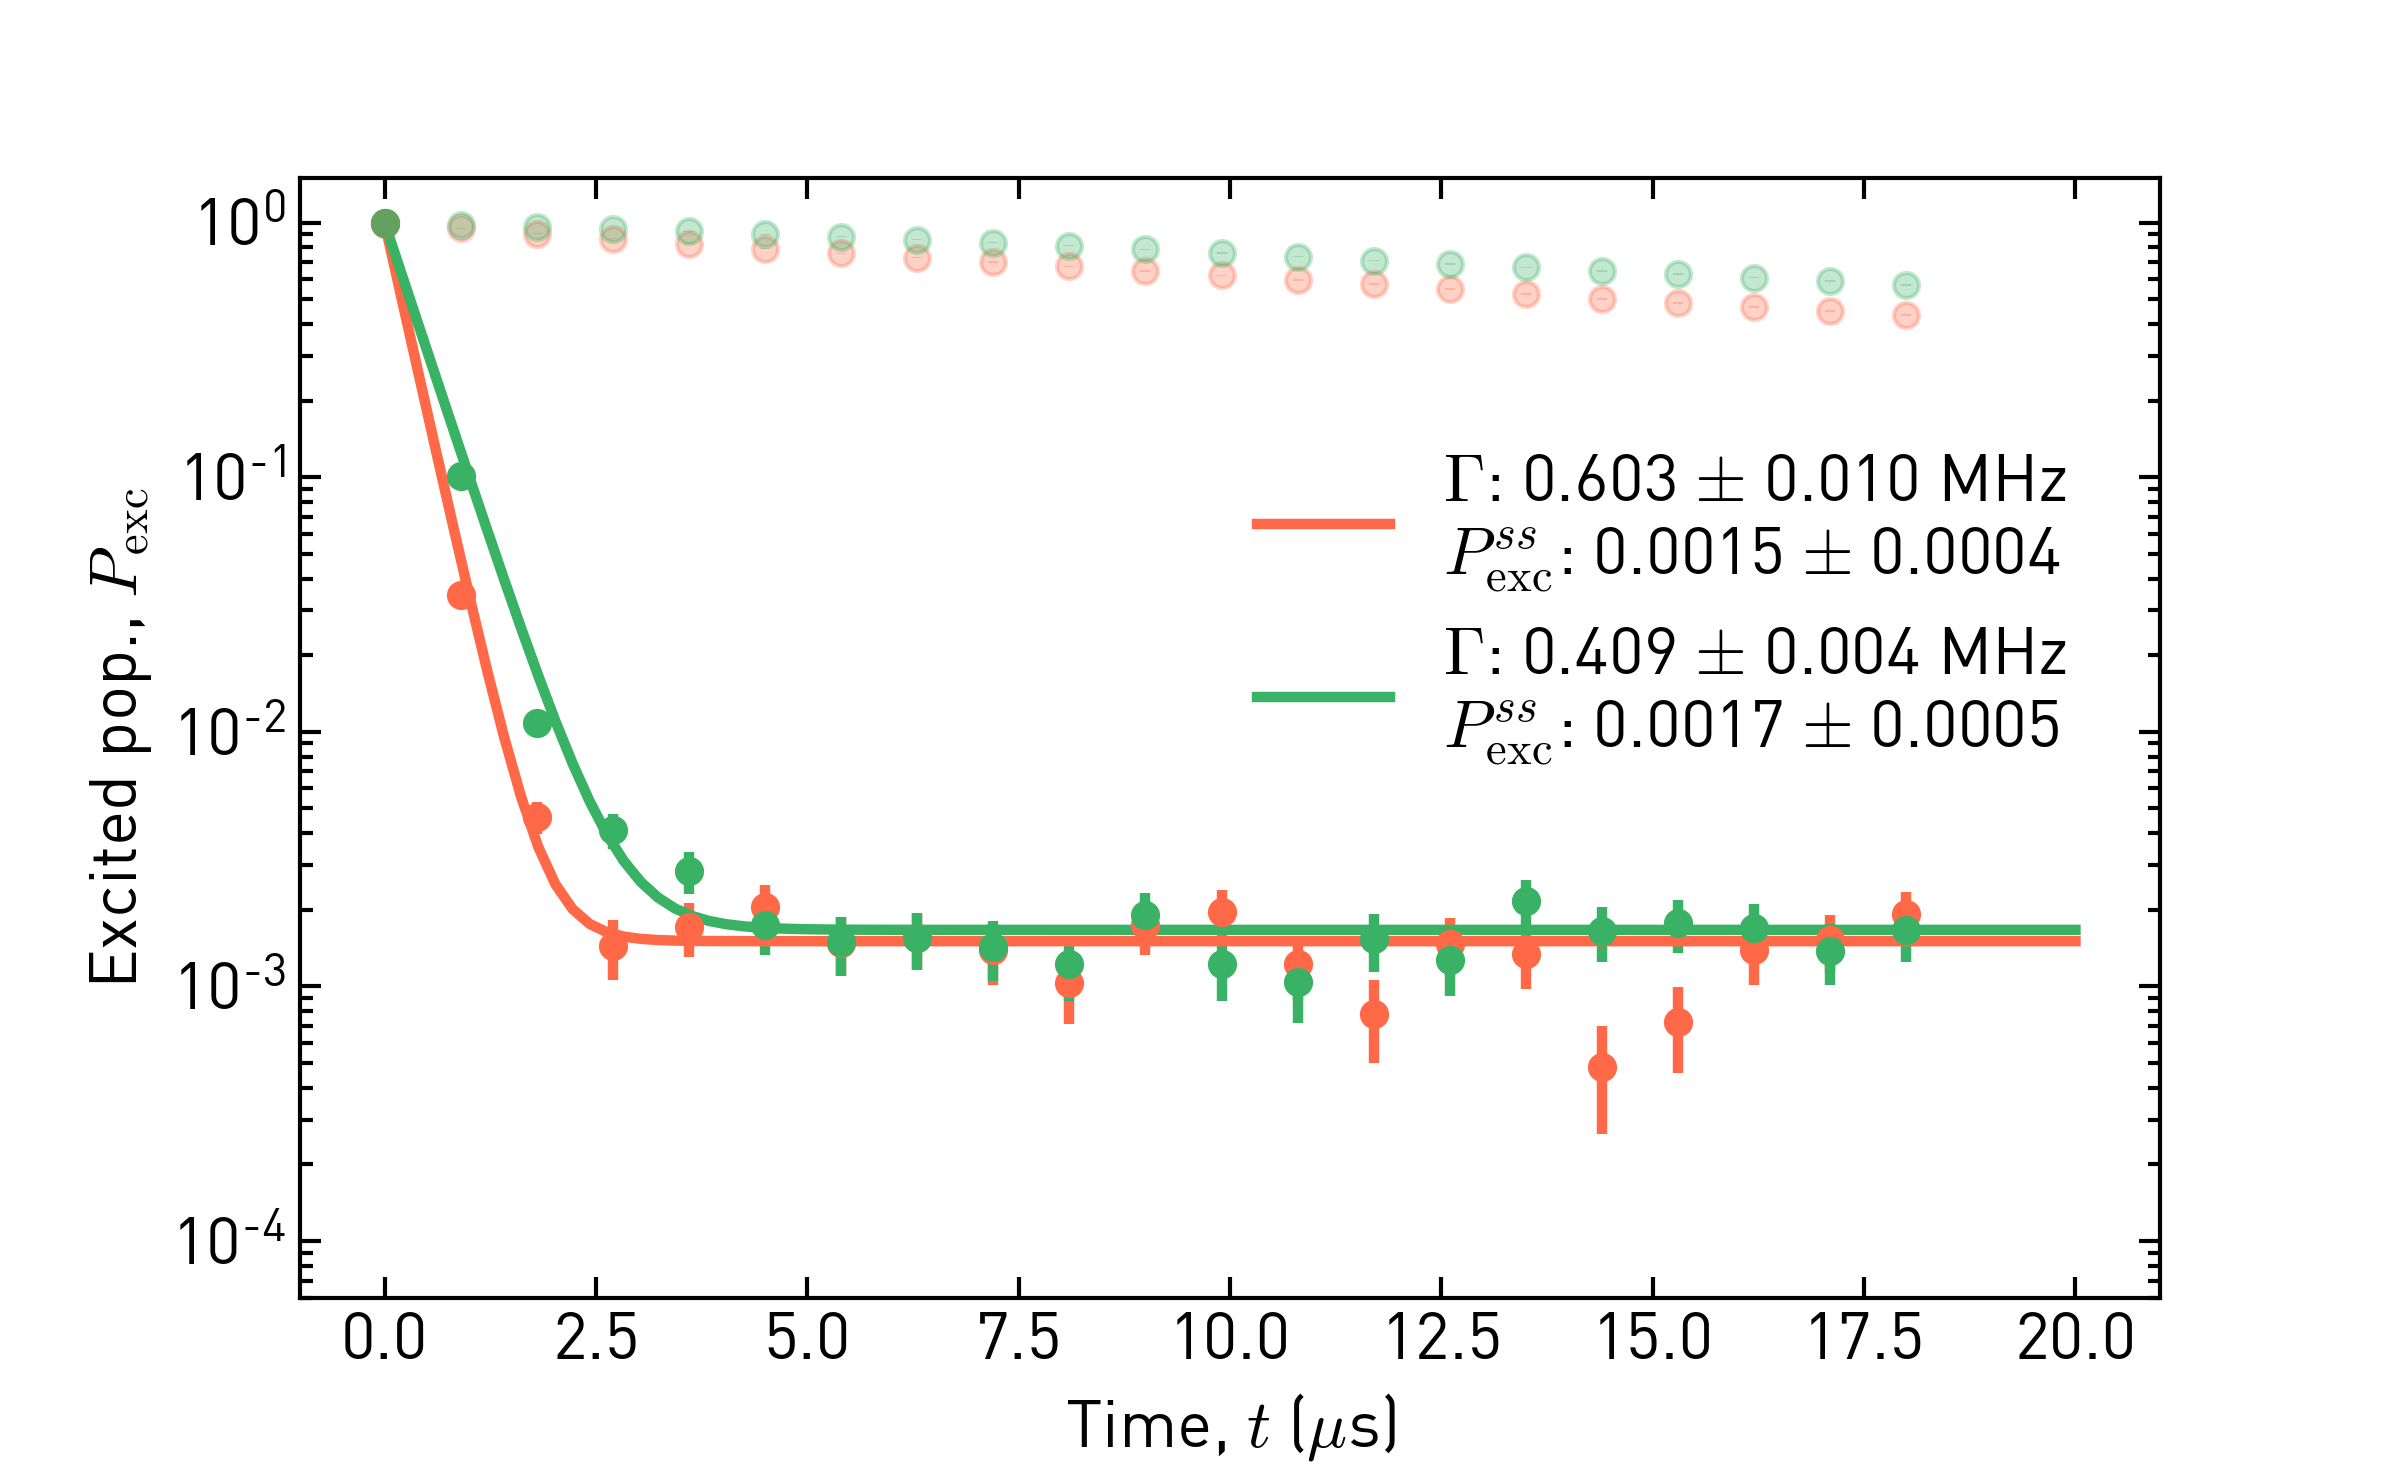
\includegraphics[width=\textwidth]{appendices/qutrit_readout/figs/ch3_readout_active_reset_fit_20200308_173706.png}
    \caption{Excited state population for a qutrit prepared in \e{} (red) and \f{} (green). The solid lines correspond to a fit to Eq.~\eqref{eq:qutrit_readout_active_reset_rate_model} to extract the reset rate and the residual, steady-state excited population. For reference, the excited state population when no reset is applied is shown in translucent colors.}
    \label{fig:qutrit_readout_active_reset_rates}
\end{figure}{}

\subsubsection{Comparison to literature}
In Fig.~\ref{fig:qutrit_readout_reset_rate_comparison}, we extend the comparison of different reset protocols presented in Ref.~\cite{Magnard2018FastQubit} in terms of reset rate and residual, steady-state population to include this work (reset on \e{} only, because not all other reset protocols include reset of \f).

\begin{figure}[ht]
    \centering
    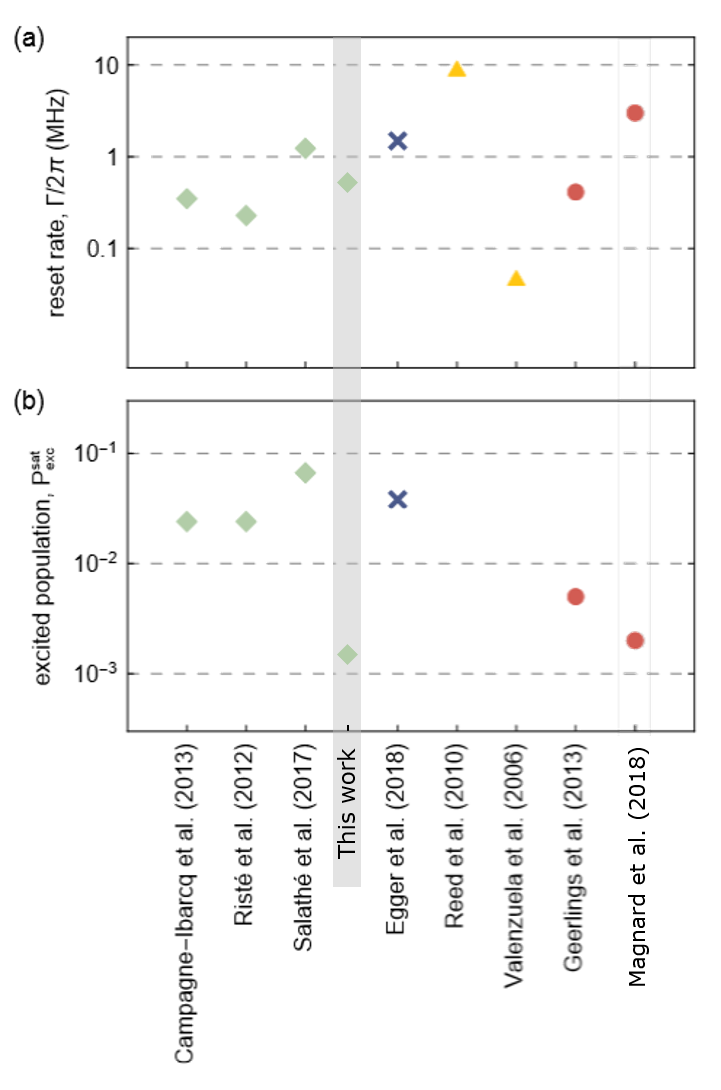
\includegraphics[width=0.5\textwidth]{appendices/qutrit_readout/figs/table_reset_rates.png}
    \caption{Comparison of reset rates $\Gamma$ (a) and residual, steady-state excited populations $P_\textrm{exc}^{ss}$ (b) of various implementations  of  qubit  reset  protocols. The protocol represented with green squares are, similarly to this work, based on qubit measurement and feedback control. We compare additional protocols based on: sequential $\pi$-pulses  to  a  dissipative  state (blue cross), qubit frequency tuning via flux pulses (yellow triangles) and all-microwave drive induced dissipation (red circles). Figure and legend reproduced and adapted from~\cite[Supplementary Material]{Magnard2018FastQubit}.}
    \label{fig:qutrit_readout_reset_rate_comparison}
\end{figure}

\subsubsection{Limitations}
There are two main limitations preventing higher reset rates. The first is the length of the feedback cycle. Indeed, the rates are inversely proportional to the time interval between two readouts: an reduction of 25\% of the feedback cycle yields an increase of 25\% of the reset rate, assuming the proportion of states assigned correctly at each time step stays constant (in fact, the proportion grows, see next paragraphs).

The second limitation on a qutrit prepared in \e{} is the decay between the second half of the readout pulse and the arrival of the feedback pulse. If the qutrit state was correctly labeled as \e{} but has decayed before the feedback pulse is applied, the feedback pulse will set the qutrit state back to \e{}. We expect 2.5-3\% of prepared states to decay during the above-mentioned time interval (615\unit{ns}) for \t{1} of 20-24\us{} which we typically observe for qubit 1. This percentage is consistent with the 3.3\% \e-state population observed after 1 feedback cycle for a qutrit prepared in \e. 

The same phenomenon limits the reset rate on a qutrit prepared in \f, however, the shorter \f-level lifetime results is more decay events within the time interval and hence a slower reset rate. 

Hence, further increase the reset rate requires a reduction of decay events which can be obtained by an increase in qutrit lifetime, or a reduction of the total latency before the feedback pulses are applied, i.e. a faster readout or an optimized \gls{uhf} firmware capable of assigning states faster. 

The main factor limiting the residual, steady-state population is the readout infidelity of the ground state, i.e. the probability of assigning \e{} or \f{} to a qutrit actually in \g. For qubit 1, the readout infidelity is 1.6\unit{\permil} which is in excellent agreement with  the observed $P_\textrm{exc}^{ss}$ of 1.5\unit{\permil} and 1.7\unit{\permil}. 

We can decrease this readout infidelity by shifting the decision thresholds further away from the mean of the ground state distribution to increase the size of the region where a state is labeled as \g{} and decrease errors caused by ground state data point located near the decision boundaries.  The ultimate population limit then becomes the re-thermalization occurring between the readout and the feedback pulse, which amounts to 0.2-0.4\unit{\permil} for qubit 1 on this device. 

Nevertheless, using more conservative thresholds for the ground state comes at a expense of increasing the probability of assigning \g{} to a qutrit actually in \e{} or \f, which in turn decreases the reset rate.

\subsubsection{Conclusion}
In this section, we have implemented a three-level, measurement-based active reset protocol yielding a reset rate of 0.60\unit{MHz} (0.41\unit{MHz}) and a residual, steady-state excited population of 1.5\unit{\permil} (1.7\unit{\permil}) for a qutrit prepared in \e{} (\f).

In addition, this reset protocol can be used at the end of any measurement sequence to reset the qutrit to its ground state, and thereby increase the measurement repetition rate by a factor of 10 compared to waiting for the natural decay of the qutrit.

The main limitation of the reset protocol is the delay between readout and the application of the feedback pulse.

Nevertheless, this reset protocol is competitive with respect to other state-of-the-art protocols and further improvement of readout circuitry, as well as electronics firmware optimization potentially allow yet better performance.






\backmatter
\chapter{Acknowledgments}
I wish to express my gratitude to Prof.~Dr.~Andreas Wallraff and Dr.~Christopher Eichler for the opportunity of performing my master thesis at the Quantum Devices Lab, as well as for the continuous feedback on my work. These months have been a wonderful journey during which I acquired a significant amount of knowledge, and met many passionate, friendly and helpful people.

I particularly thank Dr.~Christian Andersen for his precious supervision and encouragements throughout my thesis. He introduced me to experiments with quantum computers, guided many of my steps, provided detailed feedback on my writings, and always found to time to answer my countless theoretical and conceptual questions. The achievements of this thesis would not have been possible without his guidance.

I extend my gratitude to Michele Collodo for his insightful remarks on many plots presented in this thesis, for his detailed feedback on the entire manuscript of this thesis, and for the myriad of quantum physics discussions. 

I appreciate the valuable contribution of Dr.~Christoph Hellings for the QAOA project since he joined in November 2019, which include but are not limited to improvements of the QAOA measurement code, insights in understanding QAOA landscape symmetries and tuning up the 7-qubit device in preparation of larger scale QAOA experiments.

I thank Ants Remm and Stefania Lazar for the considerable amount of their time they spent to introduce me to \texttt{pycQED}, the measurement framework used for these experiments. I also acknowledge the rest of the quantum computing team for their valuable input during Monday team meetings.

From the SuperQNet team, I particularily thank Paul Magnard and Kevin Reuer for relevant discussions on three-level, single-shot readout and active reset.

I extend my thanks to Carlotta Ruppert, Bruno Lacroix, Gauthier Muguerza and Vadim Lacroix for their proofreading and feedback of the manuscript of this thesis.

Finally, I extremely grateful to Carlotta Ruppert and my family for their continuous support throughout this thesis.
% \bibliographystyle{unsrt}
% \bibliography{ressources/references}
\printbibliography
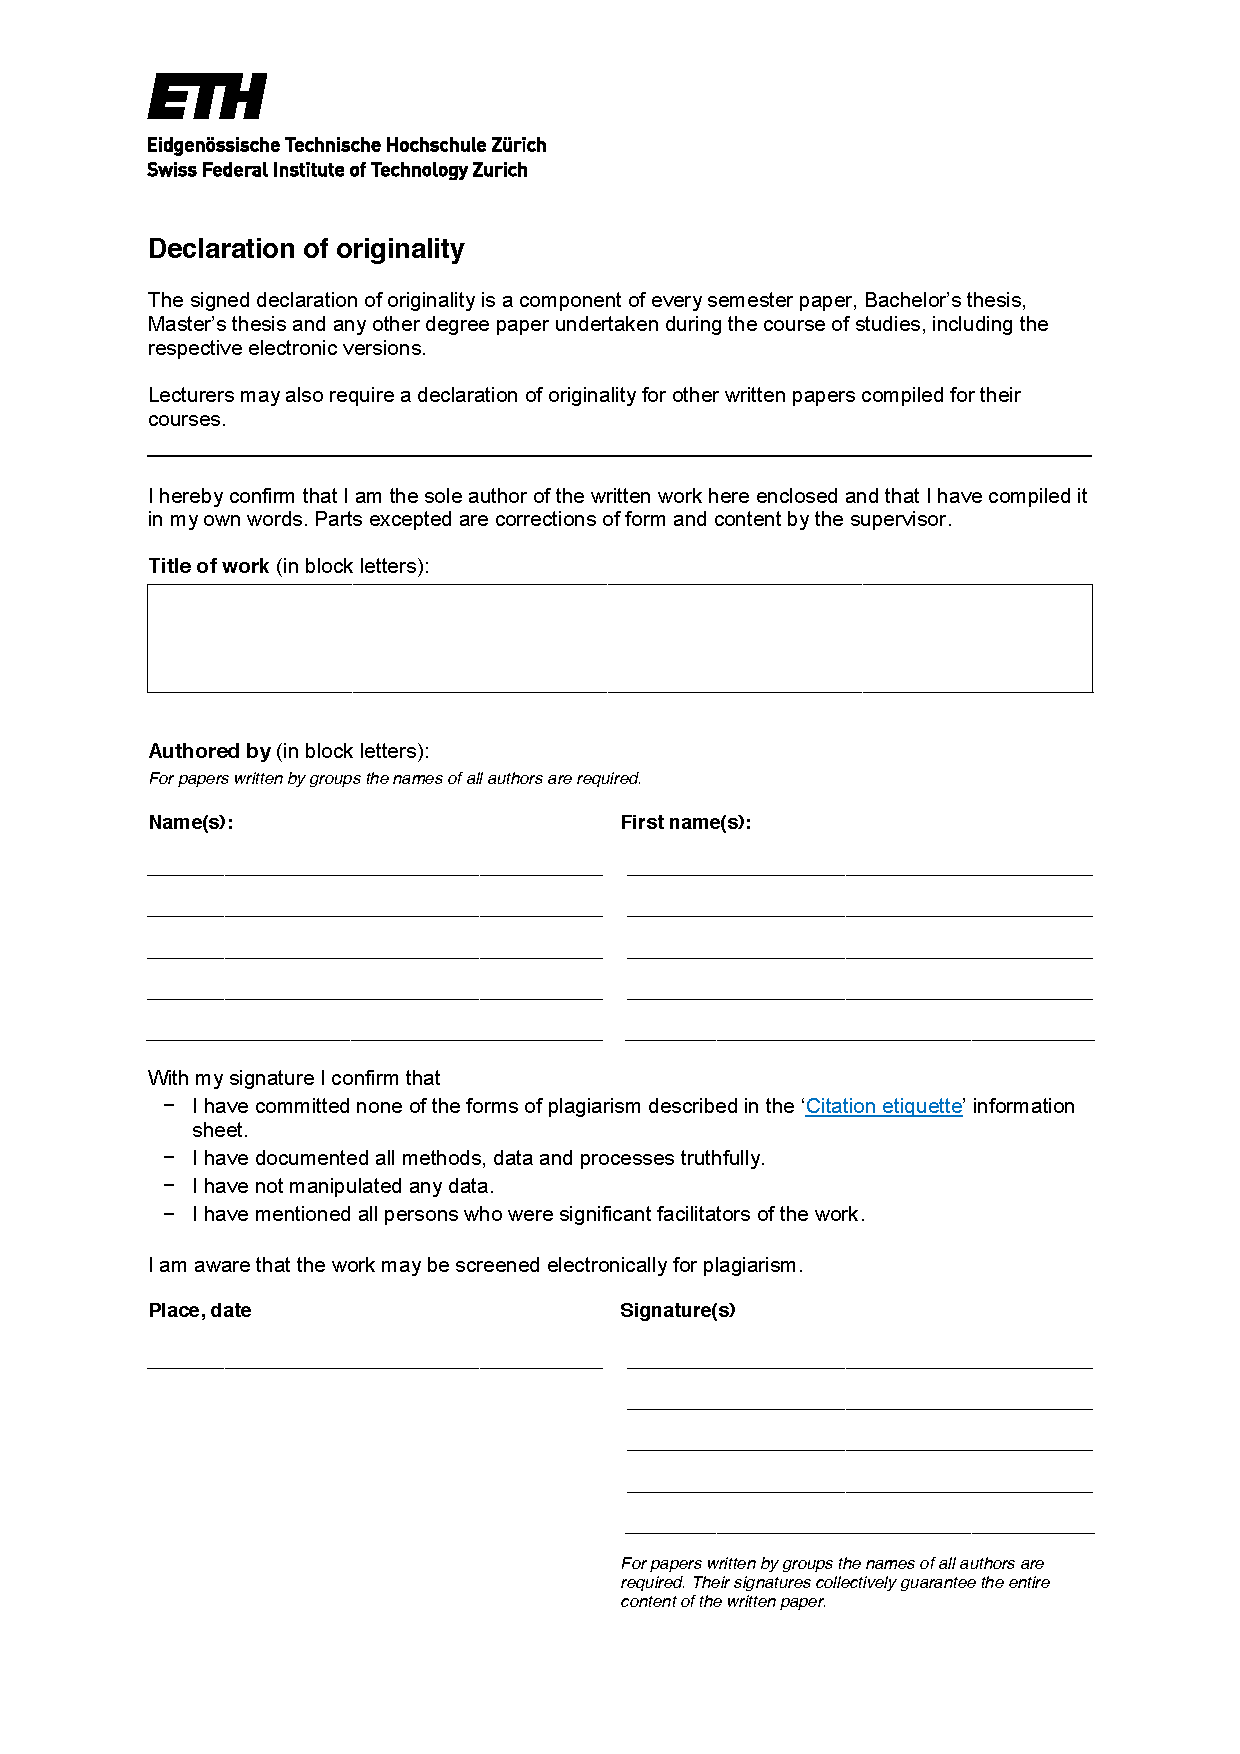
\includepdf[pages={-}]{declaration-originality.pdf}

\end{document}
